%%%%%%%%%%%%%%%%%%%%%%% file template.tex %%%%%%%%%%%%%%%%%%%%%%%%%
%
% Submissions, initial as well as final, cannot exceed 25 pages when formatted according to the two-column LaTeX template. No space-saving tricks are permitted, and all content, e.g., figures, should use font sizes that are similar to that of the running text. 
% This is a general template file for the LaTeX package SVJour3
% for Springer journals.          Springer Heidelberg 2010/09/16
%
% Copy it to a new file with a new name and use it as the basis
% for your article. Delete % signs as needed.
%
% This template includes a few options for different layouts and
% content for various journals. Please consult a previous issue of
% your journal as needed.
%
%%%%%%%%%%%%%%%%%%%%%%%%%%%%%%%%%%%%%%%%%%%%%%%%%%%%%%%%%%%%%%%%%%%
%=
% First comes an example EPS file -- just ignore it and
% proceed on the \documentclass line
% your LaTeX will extract the file if required
\begin{filecontents*}{example.eps}
%!PS-Adobe-3.0 EPSF-3.0
%%BoundingBox: 19 19 221 221
%%CreationDate: Mon Sep 29 1997
%%Creator: programmed by hand (JK)
%%EndComments
gsave
newpath
  20 20 moveto
  20 220 lineto
  220 220 lineto
  220 20 lineto
closepath
2 setlinewidth
gsave
  .4 setgray fill
grestore
stroke
grestore
\end{filecontents*}
%
\RequirePackage{fix-cm}
%
%\documentclass{svjour3}                     % onecolumn (standard format)
%\documentclass[smallcondensed]{svjour3}     % onecolumn (ditto)
%\documentclass[smallextended]{svjour3}       % onecolumn (second format)
\documentclass[twocolumn]{svjour3}          % twocolumn
%
\smartqed  % flush right qed marks, e.g. at end of proof
%
\usepackage[numbers,sort&compress]{natbib}
\usepackage{amsmath,amssymb}
\DeclareMathOperator*{\argmin}{argmin} 
\DeclareMathOperator*{\argmax}{argmax}
\usepackage{graphicx}
\usepackage{enumerate}
\usepackage{booktabs}
\usepackage[ruled, vlined, linesnumbered]{algorithm2e}
\usepackage{balance}
\usepackage{caption}
\usepackage{subcaption}
\captionsetup[subfigure]{skip=0pt}
% \captionsetup[figure]{font=small}
% \captionsetup[table]{font=small}
%\usepackage{subfig}
\usepackage{xcolor}
\usepackage{multirow}
\usepackage{mathrsfs}
\usepackage{epstopdf}
\usepackage{xspace}
\usepackage{afterpage}
\usepackage{listings}
\usepackage{makecell}
\usepackage{threeparttable}
\usepackage{cases}
% \usepackage{enumitem}
% \setlist[itemize]{leftmargin=1em}
\lstset{
  breaklines=true,                           
  language=SQL,
  frame=none,
  framesep=0pt,
  xleftmargin=-2ex,
  showspaces=false, 
  showtabs=false, 
  tabsize=1,
  showstringspaces=false, 
  breakatwhitespace=false, 
  showtabs=false,
  basicstyle=\ttfamily\small,
  keywordstyle=\ttfamily\bfseries,
  identifierstyle=\ttfamily,
  stringstyle=\ttfamily,
}



\newlength{\oldtextfloatsep}\setlength{\oldtextfloatsep}{\textfloatsep}
\newlength{\oldfloatsep}\setlength{\oldfloatsep}{\floatsep}
\newcommand{\tabincell}[2]{\begin{tabular}{@{}#1@{}}#2\end{tabular}}
\newcommand{\critBig}{\text{Strategy}}
\newcommand{\crit}{\text{strategy}}
\newcommand{\critplu}{\text{strategies}}
\newcommand{\ie}{\emph{i.e.},\xspace}
\newcommand{\eg}{\emph{e.g.},\xspace}
\newcommand{\etc}{\emph{etc.}\xspace}
\newcommand{\aka}{\emph{a.k.a.}\xspace}
\newcommand{\etal}{\emph{et al.}\xspace}
\newcommand{\cf}{cf.\/~}
\newcommand\figref[1]{Fig.~\ref{#1}}
\newcommand\figsubref[1]{Fig.~\subref{#1}}
\newcommand\tabref[1]{Table~\ref{#1}}
\newcommand\tabsubref[1]{Table~\subref{#1}}
\newcommand\secref[1]{Sec.~\ref{#1}}
\newcommand\equref[1]{Eq.~(\ref{#1})}
\newcommand\appref[1]{Appendix~\ref{#1}}
\newcommand\algref[1]{Alg.~\ref{#1}}
\newcommand\expref[1]{Example~\ref{#1}}
\newcommand\lemref[1]{Lemma~\ref{#1}}
\newcommand\defref[1]{Def.~\ref{#1}}
\newcommand{\fakeparagraph}[1]{\vspace{0mm}\noindent\textbf{#1.}}

\ifodd 0
\newcommand{\zeng}[1]{{\color{blue}{#1}}}
\newcommand{\rev}[1]{{\color{blue}{#1}}}
\newcommand{\Fan}[1]{{\color{magenta}{#1}}}
\newcommand{\Song}[1]{{\color{cyan}{#1}}}
\else
\newcommand{\zeng}[1]{#1}
\newcommand{\Fan}[1]{#1}
\newcommand{\Song}[1]{#1}
\newcommand{\rev}[1]{#1}
\fi

%% specifically defined in this paper
\newcommand{\gc}{SMCQL}
\newcommand{\sss}{Conclave}
\newcommand{\he}{S-kNN}
\newcommand{\thres}{r}
\newcommand{\Cand}{Cand}
\newcommand{\kdist}{d^{k}}
\newcommand{\sysname}{\text{Hu-Fu}\xspace}
\newcommand{\ssum}{\textsf{SUM}\xspace}
\newcommand{\dist}{\textsf{dist}\xspace}
\newcommand{\scmp}{\textsf{CMP}\xspace}
\newcommand{\ssun}{\textsf{SUN}\xspace}
\newcommand{\sdcmp}{\textsf{DCMP}\xspace}
\newcommand{\geoi}{\textsf{GeoI}\xspace}
\newcommand{\Prob}{\mathrm{Pr}\xspace}
\newcommand{\lrc}{\textsf{RC}\xspace}
\newcommand{\lrq}{\textsf{RQ}\xspace}
\newcommand{\TRQ}{T_{\lrq}}
\newcommand{\TRC}{T_{\lrc}}
\newcommand{\knn}{\textsf{kNN}\xspace}
\newcommand{\FRQ}{\textsf{FRQ}\xspace}
\newcommand{\FRC}{\textsf{FRC}\xspace}
\newcommand{\FDJ}{\textsf{FDJ}\xspace}
\newcommand{\FKNN}{\textsf{FNN}\xspace}
\newcommand{\FKNNJ}{\textsf{FNNJ}\xspace}
\newcommand{\smcql}{SMCQL-GIS\xspace}
\newcommand{\public}{Public\xspace}
\newcommand{\conclave}{Conclave-GIS\xspace}
\newcommand{\conclaveext}{Conclave-GISext\xspace}
\newcommand{\smcqlext}{SMCQL-GISext\xspace}
\newcommand{\mpconclave}{Conclave-MP\xspace}
\newcommand{\EDBT}{LFHE\xspace}
\newcommand{\ICDE}{PINED-RQ++\xspace}

%
% \usepackage{mathptmx}      % use Times fonts if available on your TeX system
%
% insert here the call for the packages your document requires
%\usepackage{latexsym}
% etc.
%
% please place your own definitions here and don't use \def but
% \newcommand{}{}
%
% Insert the name of "your journal" with
% \journalname{myjournal}
%
\begin{document}

\title{\sysname: Efficient and Secure Spatial Queries over Data Federation}
% \subtitle{Do you have a subtitle?\\ If so, write it here}

%\titlerunning{Short form of title}        % if too long for running head

\author{
    Yongxin Tong $^1$ \and
	Yuxiang Zeng $^1$ \and
    Yang Song $^1$ \and
	Xuchen Pan $^1$ \and
	Zeheng Fan $^1$ \and
	Chunbo Xue $^1$ \and 
	Zimu Zhou $^2$ \and 
	Xiaofei Zhang $^3$ \and
	Lei Chen $^4$ \and
	Yi Xu $^1$ \and 
	Ke Xu $^1$ \and
	Weifeng Lv $^1$
}

\authorrunning{Yongxin Tong, Yuxiang Zeng, Yang Song, et al.} % if too long for running head

\institute{
        Y. Tong 
              \email{yxtong@buaa.edu.cn}           
           \and \\
           Y. Zeng 
              \email{yxzeng@buaa.edu.cn}
			\and \\
         Y. Song \email{songyangbuaa@buaa.edu.cn}
           \and \\
         X. Pan \email{panxuchen@buaa.edu.cn}
           \and \\
			Z. Fan 
              \email{fanzh@buaa.edu.cn}
			\and \\
			C. Xue 
              \email{xuechunbo@buaa.edu.cn}
			\and \\
			Z. Zhou 
              \email{zimuzhou@cityu.edu.cn}
			\and \\
			 X. Zhang
           		\email{xiaofei.zhang@memphis.edu}
			\and \\
           L. Chen
           		\email{leichen@cse.ust.hk}
			\and \\
           Y. Xu
              \email{xuy@buaa.edu.cn}          %  \\
			\and \\
			K. Xu
              \email{kexu@buaa.edu.cn}          %  \\
			\and \\
			W. Lv
              \email{lwf@buaa.edu.cn} \\
        $^1$ State Key Laboratory of Complex \& Critical Software Environment and Beijing Advanced Innovation Center for Future Blockchain and Privacy Computing, Beihang University \\
        $^2$ School of Data Science, City University of Hong Kong \\
        $^3$ The University of Memphis \\
        $^4$ The Hong Kong University of Science and Technology (GZ) and The Hong Kong University of Science and Technology \\
}

% \institute{
% Y. Tong \at
%               SKLCCSE, Beijing Advanced Innovation Center for Future Blockchain and Privacy Computing, Beihang University \\
%               \email{yxtong@buaa.edu.cn}           %  \\
%            \and
   %         X. Pan \at
   %            Beihang University
   %            \email{panxuchen@buaa.edu.cn}          %  \\
   %         \and
   %         Y. Zeng \at
   %         	  SKLCCSE, Beijing Advanced Innovation Center for Future Blockchain and Privacy Computing, Beihang University \\
   %            \email{yxzeng@buaa.edu.cn}          %  \\
			% \and
			% Y. Shi \at
   %         	 Beihang University 
   %            \email{skyxuan@buaa.edu.cn}          %  \\
			% \and
			% C. Xue \at
   %         	  Beihang University
   %            \email{xuechunbo@buaa.edu.cn}          %  \\
			% \and
			% Z. Zhou \at
   %         	  School of Data Science, City University of Hong Kong \\
   %            \email{zimuzhou@cityu.edu.cn}          %  \\
			% \and
			%  X. Zhang \at
   %         	  University of Memphis
   %         		\email{xiaofei.zhang@memphis.edu}
			% \and
           % L. Chen \at
           % 	 The Hong Kong University of Science and Technology (GZ) and The Hong Kong University of Science and Technology \\
           % 		\email{leichen@cse.ust.hk}
			% \and
   %         Y. Xu \at
   %         	  SKLCCSE, Beijing Advanced Innovation Center for Future Blockchain and Privacy Computing, Beihang University \\
   %            \email{xuy@buaa.edu.cn}          %  \\
			% \and
			% K. Xu \at
   %         	  SKLCCSE, Beijing Advanced Innovation Center for Future Blockchain and Privacy Computing, Beihang University \\
   %            \email{kexu@buaa.edu.cn}          %  \\
			% \and
			% W. Lv \at
   %         	  SKLCCSE, Beijing Advanced Innovation Center for Future Blockchain and Privacy Computing, Beihang University \\
   %            \email{lwf@buaa.edu.cn}          %  \\
% }

\date{Received: date / Accepted: date}
% The correct dates will be entered by the editor


\maketitle

\begin{abstract}
    Data isolation has become an obstacle to scale up query processing over big data, since sharing raw data among data owners is often prohibitive due to security concerns.
    A promising solution is to perform secure queries over a federation of multiple data owners leveraging secure multi-party computation (SMC) techniques, as evidenced by recent federation studies on relational data.
    However, existing solutions are highly inefficient on spatial queries due to excessive secure distance operations for query processing and their usage of general-purpose SMC libraries for secure operation implementation. 
    In this paper, we propose \sysname, the first system for efficient and secure spatial query processing on a data federation. 
    \sysname seamlessly supports five mainstream spatial queries at scale, while ensuring both data and query privacy (\ie sensitive spatial information of data owners and query users).
    The idea is to decompose the secure processing of a spatial query into as many plaintext operations and as few secure operations as possible, where fewer secure operators are involved and all of them are implemented dedicatedly.
    As a working system, \sysname supports not only query input in native SQL, but also heterogeneous spatial databases (\eg PostGIS, GeoMesa, and SpatialHadoop) at the backend.
    Extensive experiments show that \sysname usually outperforms the state-of-the-arts in running time and communication cost while guaranteeing security.
    \keywords{Federated database \and Spatial database \and Query processing \and Data privacy}
\end{abstract}
        
\section{Introduction}
\label{sec:intro}

Efficient processing of spatial queries over large-scale data is essential for a wide spectrum of smart city applications, such as taxi-calling~\cite{DBLP:conf/kdd/Ye19} and logistics planning~\cite{DBLP:journals/pvldb/ZengTC19}.
Although the volume of spatial data continues to grow, it becomes increasingly difficult for these applications to take full advantage of the big spatial data due to the data isolation problem (\aka isolated data) \cite{DBLP:journals/debu/TongZZLSL0L23, DBLP:journals/fcsc/LiuZSTZ24, DBLP:journals/fcsc/SunWTL24}.
Spatial datasets at city or nation scale are often privately possessed and separately owned by multiple parties, where sharing raw data among parties or uploading raw data to a third party (\eg a cloud) is prohibitive due to legal regulations (\eg GDPR \cite{voigt2017eu}) or commercial reasons.

A promising paradigm to tackle the data isolation problem is to perform \textit{secure} queries over a \textit{data federation} \cite{vldb17smcql}, which consists of multiple data owners (\aka data silos) who agree on the same schema and manage their own data autonomously. 
Note that this paradigm differs from conventional federated databases \cite{DBLP:books/sp/OzsuV20} in the extra security requirement.
In general, secure query processing over data federation can be solved by well-known techniques such as secure multi-party computation (SMC) \cite{DBLP:journals/ftsec/EvansKR18}.
Yet, only recently did pioneer studies such as SMCQL~\cite{vldb17smcql} and Conclave~\cite{eurosys19conclave} take the first step towards practice with efficient query execution plans upon SMC libraries for (relational) data federation.
Unsurprisingly, more applications are being built on federations of spatial data owners.

\begin{example}
AMAP \cite{AMAP} (GaoDe Map in China) has united over $8$ Chinese travel companies into an integrated taxi-calling platform to offer users the taxis resources from all participating companies.
A spatial data federation can protect the distribution of taxis' locations of each company (\ie data silo), which could be a business secret, from leaking to others.
This privacy concern for data silos is commonly referred to as \textit{data privacy} \cite{DBLP:reference/dbsec/2008}.
\end{example}

\begin{example}
During COVID-19, several mobile network operators (\eg China Mobile~\cite{chinamobile} and China Telecom~\cite{chinatelecom}) cooperated as a data federation to identify individuals who had contacts with infectious patients through their location data~\cite{contact}.
Executing spatial queries (\eg range query) over a data federation helps identify contacts of infectious patients across multiple organizations' spatial data without compromising privacy.
Here, strict privacy requirements go beyond the data privacy since the locations of patients, which appear in queries, also need protections.
The privacy concern for spatial data in queries is referred to as \textit{query privacy} \cite{DBLP:reference/dbsec/2008}.
\end{example}

\rev{Due to legal regulations (\eg GDPR \cite{voigt2017eu}), protecting \textit{data privacy} is now common in real-life scenarios, 
especially when spatial location implies the travel patterns or personal trajectories of a user. 
\textit{Query privacy} is equally important, 
but perhaps gets less attention in existing research on data federation. 
Query privacy also has numerous real-world applications \cite{DBLP:reference/sp/2018mdp,DBLP:conf/esorics/2009-5599},
such as navigation, location-based social networking, location-based advertising, and POI search \footnote{Please refer to \appref{app:query-privacy-app} for more detailed explanations on these application scenarios}.}

Nevertheless, directly adapting the state-of-the-art data federation solutions~\cite{vldb17smcql, eurosys19conclave} to spatial data can be inefficient.
From our empirical study (\secref{subsec:challenges}) of a kNN query on a real dataset, they are at least $142 \times$ slower, and have at least $1,216\times$ higher communication cost than plaintext query processing.
There are two reasons for such inefficiency.
\textit{(i)}
Existing solutions process spatial queries with excessive secure distance operations, which occupy over 90\% of the time cost.
For example, SMCQL~\cite{vldb17smcql} and Conclave~\cite{eurosys19conclave} would securely sort spatial objects by distances to the query point and pick the top-k objects, where each sorting involves numerous secure distance comparisons.
\textit{(ii)}
Previous studies \cite{vldb17smcql,eurosys19conclave} are built on general-purpose SMC libraries, which may sacrifice the efficiency of specific operations for other considerations.
For example, our experiment shows that the secure summation in ObliVM~\cite{DBLP:conf/sp/LiuWNHS15}, the SMC library adopted by SMCQL~\cite{vldb17smcql}, can be accelerated by $15\times$ via dedicated implementations~\cite{DBLP:journals/dke/EmekciSAA07}.

In this paper, we aim at efficient and secure spatial queries over a data federation, which we call \textit{federated spatial queries}.
We mainly study five queries (federated range query, range counting, kNN query, distance join, and kNN join) commonly seen in spatial database research~\cite{sigmod16simba,icde15spatialhadoop} and follow the semi-honest adversary model adopted by previous work \cite{vldb17smcql, eurosys19conclave, DBLP:conf/sigmod/Wang021}.
Moreover, we develop a more practical solution than \cite{vldb17smcql, eurosys19conclave} by eliminating the need for an honest broker and supporting more data silos (these studies support at most three data silos whereas we tested up to ten).

To this end, we propose \sysname \cite{fullpaper}, a system for efficient and secure processing of federated spatial queries.
As explained above, secure operations are usually slow and easily become the efficiency bottleneck.
Thus, the \textbf{key idea} of \sysname is to decompose a federated spatial query into as many plaintext operations while minimizing secure distance-related operations without compromising privacy.
The decomposition aims to achieve two goals: \textit{(i)} reduce the number of distance-related operations to the minimum, and \textit{(ii)} implement secure operations faster than those in general-purpose SMC libraries.
To realize this idea and implement a practical system, \sysname consists of three components: an query rewriter with novel decomposition plans, a set of drivers adaptable to heterogeneous databases and an easy-to-use query interface with SQL support.
Specifically, the query rewriter identifies a set of plaintext and secure operators for the query execution plan to handle the queries of interest. It ensures diverse privacy requirements, as explained in Examples 1 and 2: data privacy only, or both data and query privacy. 
The drivers provide implementations of secure operators with dedicated SMC protocols and plaintext operators as interfaces on top of the heterogeneous spatial databases adopted by different data silos. The query interface supports spatial queries in native SQL for easy usage.

\fakeparagraph{Contribution}
Our main contributions and results are summarized as follows.
\begin{itemize}%[noitemsep,topsep=0pt]
	\item 
	To the best of our knowledge, \sysname is the first system on efficient and secure spatial queries over a data federation, and is also available on GitHub \cite{fullpaper}.
    \item 
    We devise novel decomposition plans for federated spatial queries. 
    After decomposition, an execution plan involves only a limited number of secure operators that can be effectively supported with fast and dedicated implementations.
    \item 
    \sysname is an efficient, easy-to-use system that supports query input in SQL and heterogeneous spatial databases, \eg PostGIS~\cite{postgis}, Simba~\cite{sigmod16simba}, GeoMesa~\cite{ds15geomesa}, SpatiaLite~\cite{spatialite}, 
    and SpatialHadoop~\cite{icde15spatialhadoop}.
    \item 
    Extensive evaluations show that \sysname usually outperforms the state-of-the-arts \cite{vldb17smcql, eurosys19conclave} in efficiency.
	Compared with two strong baselines, namely \smcql and \conclave, which are extended from SMCQL \cite{vldb17smcql} and Conclave \cite{eurosys19conclave} to spatial queries, \sysname is up to 4 orders of magnitude faster and 5 orders of magnitude lower in communication overhead than \smcql and \conclave with the same security level.
\end{itemize}

Compared with the preliminary version \cite{DBLP:journals/pvldb/TongPZSXZZCXXL22} of this work, we have made the following new contributions.
\textit{(i)} We expand our scope to a new and challenging setting where both data and query privacy must be preserved. 
\sysname also provides the corresponding SQL \textit{query interface}.
\textit{(ii)} The \textit{query rewriter} is extended and optimized to handle all five spatial queries in this new setting.
\textit{(iii)} In \textit{drivers}, two additional secure operators are tailored to fulfill the extra privacy requirement.
\textit{(iv)} Extensive evaluations are conducted to show the performance.

\fakeparagraph{Roadmap}
In the rest of this paper, we define our problem scope and identify the inefficiency of existing solutions in \secref{sec:statement}. We present an overview of \sysname in \secref{sec:overview} and elaborate on the three functional components in \secref{sec:rewriter}, \secref{sec:drivers}, and \secref{sec:interface}.
Finally, we present the evaluations in \secref{sec:evaluations}, review the related work in \secref{sec:related}, and conclude in \secref{sec:conclusion}.

\section{Problem Statement}
\label{sec:statement}

This section clarifies our problem scope and highlights the technical challenges when developing \sysname.

\subsection{Problem Scope}
\label{subsec:problem}

A data federation $F$ (``federation'' as short) consists of $n$ data silos $\{F_i\}$ (``silos'' as short), where each silo holds massive \textit{spatial objects}.
Each spatial object $o$ has a location $l_o$ and (optionally) other attributes.
The federation supports \textit{federated spatial queries} over the spatial objects of all silos under the following settings.
\begin{itemize}
    \item \textbf{Spatial Queries.}
    The federation supports mainstream spatial queries like range query, range counting, kNN query, distance join, and kNN join~\cite{DBLP:series/synthesis/2011Mamoulis,sigmod16simba}.
    
    \item \textbf{Autonomous Databases.} 
    Each data silo is an autonomous database that manages (\eg deletes and inserts its own spatial objects and prohibits sharing its spatial objects in plaintext with the other data silos \cite{vldb17smcql, eurosys19conclave, DBLP:journals/pvldb/BaterHEMR18, DBLP:journals/pvldb/BaterP0WR20}.
    
    \item \textbf{Semi-honest Adversaries.} 
    Each silo honestly executes queries received and returns authentic results, but may attempt to infer data from other silos during query execution.
	This assumption is common in query processing over a data federation \cite{vldb17smcql, eurosys19conclave, DBLP:journals/pvldb/BaterHEMR18, DBLP:journals/pvldb/BaterP0WR20}.
\end{itemize}

Moreover, the query processing methods should consider the following requirements thoughtfully.
\begin{itemize}
	\item \textbf{Efficiency Requirements.}
	We care about the \textit{running time} and \textit{communication cost} to execute \textit{exact} queries over multiple silos.
    Short running time is often desirable since real-life applications may process massive queries and expect prompt responses.
	Minimal communication cost is critical in distributed query processing \cite{DBLP:books/sp/OzsuV20} and secure query processing \cite{DBLP:reference/dbsec/2008}.
	Approximate query processing over data federation \cite{DBLP:journals/pvldb/BaterP0WR20,DBLP:conf/sigmod/ChowdhuryW0MJ20,DBLP:conf/dasfaa/ZhangTSZXCZXLZ23} is out of our scope because applications such as contact tracing require accurate results.
	We consider multiple silos as aligned with real-world applications.
	Similar to existing solutions \cite{vldb17smcql, eurosys19conclave}, the storage efficiency, which mainly depends on silos themselves, is not our primary concern.
 
    \item \textbf{Privacy Requirements.}
    We consider \textit{two} different types of privacy requirements \cite{DBLP:reference/dbsec/2008,DBLP:journals/ftsec/EvansKR18}.
    \begin{enumerate}[(1)]
    \item \textit{Data privacy}: each data silo should not deduce any sensitive data from others, and no additional sensitive data should be revealed to the query user, except for the final query answer.
    \item \textit{Query privacy} (optional): the spatial location of a user's query cannot be revealed to data silos.
    \end{enumerate}
\end{itemize}

\fakeparagraph{Remark}
In practice, the need for query privacy may vary across applications.
For example, in scenarios such as a passenger requesting a taxi-calling service through AMAP \cite{AMAP}, query privacy may be unnecessary. 
This is because the platform ultimately needs to know the passenger's pickup location.
Conversely, in situations like performing contact tracings based on a patient's location, query privacy becomes crucial to prevent the disclosure of sensitive spatial information to data silos. 
For ease of presentation, we classify federated spatial queries into two kinds: 
\textit{asymmetric queries} (which require data privacy only) and \textit{symmetric queries} (which require both data privacy and query privacy).

To satisfy the privacy requirements, 
some existing systems \cite{vldb17smcql,eurosys19conclave} assume the existence of a trusted broker responsible for collecting partial answers, which may contain sensitive data, from each silo.
In reality, even if brokers (\eg Acxiom~\cite{acxiom}) charge high fees for their data broker services, there is still a risk of them leaking sensitive data for personal gain \cite{broker}.
Thus, we explore solutions without reliance on a trusted broker.

\subsection{Main Challenges}
\label{subsec:challenges}

Federated queries can be realized by secure multi-party computation (SMC) \cite{DBLP:journals/ftsec/EvansKR18}, as in prior studies for relational data \cite{vldb17smcql, eurosys19conclave}.
Nevertheless, our empirical study shows that they are highly inefficient on spatial queries.

\subsubsection{Inefficiency on Federated Spatial Queries}
\label{subsubsec:inefficiency}

As an illustrative study, we perform an asymmetric federated kNN query by extending SMCQL \cite{vldb17smcql} and Conclave \cite{eurosys19conclave}, two representative solutions to secure query processing on (relational) data federations.

\fakeparagraph{Overview of Existing Solutions}
The common framework \cite{vldb17smcql,eurosys19conclave} for secure query processing over a data federation decomposes query execution into \textit{plaintext} queries within each silo and \textit{secure} computations of the partial results across silos.
Existing solutions differ in the SMC techniques used for secure operations, with garbled circuits (GC) and secret sharing (SS) as the mainstreams \cite{DBLP:journals/ftsec/EvansKR18}.
For example, \smcql \cite{vldb17smcql} uses a prevalent GC based library, ObliVM~\cite{DBLP:conf/sp/LiuWNHS15}, to support two silos.
\conclave \cite{eurosys19conclave} adopts an SS based technique (Sharemind~\cite{DBLP:conf/esorics/BogdanovLW08}), which enables query processing on three silos.

\fakeparagraph{Setup}
\smcql \cite{vldb17smcql} and \conclave \cite{eurosys19conclave} are extended to asymmetric federated kNN queries as follows.
Following the ``plaintext + secure'' processing pipeline, each silo first conducts a plaintext kNN query and returns the $k$ nearest points (along with their distances) to the query point.
Then, the final kNNs are derived by a top-$k$ operation from these returned points, which are securely sorted by their distances to the query point.
We experiment with two silos with $k = 16$.
Other details of experimental setups are elaborated in \secref{sec:experiment-setup}.

\fakeparagraph{Result}
\figref{fig:cmp-k} plots the (average) running time and communication cost to process an asymmetric federated kNN query leveraging existing solutions \cite{vldb17smcql, eurosys19conclave}.
The results are averaged over $50$ queries.
Compared with \public, \ie plaintext kNN query execution without any privacy protection, the secure counterpart incurs $142\times$ to $212\times$ longer running time and $1,216\times$ to $22,510\times$ higher communication cost.
Although the method \smcql yields shorter running time and lower communication overhead than \conclave,
it is \textit{limited to scenarios with only two silos} due to its reliance on garbled circuits (GC).
Yet it still takes $2.86$ seconds to answer a federated spatial query, which can hurt user experiences in applications where query time efficiency is critical.

\begin{table}[t]
    \centering
    \caption{Percentage of time spent for \textit{plaintext} or \textit{secure} operations in an asymmetric federated kNN query.}
    \label{tab:breakdown}
    \begin{small}
    \begin{tabular}{lll}
    \toprule
    \textbf{Existing Solution} & \textbf{Plaintext} & \textbf{Secure} \\ 
    \midrule
    \smcql \cite{vldb17smcql} & $0.14\%$ & $99.86\%$ \\
    \conclave \cite{eurosys19conclave} & $0.10\%$ & $99.90\%$ \\
    \bottomrule
    \end{tabular}
    \end{small}
\end{table}

\begin{figure}[t]
    \centering
    \begin{subfigure}{0.228\textwidth}
        \centering
        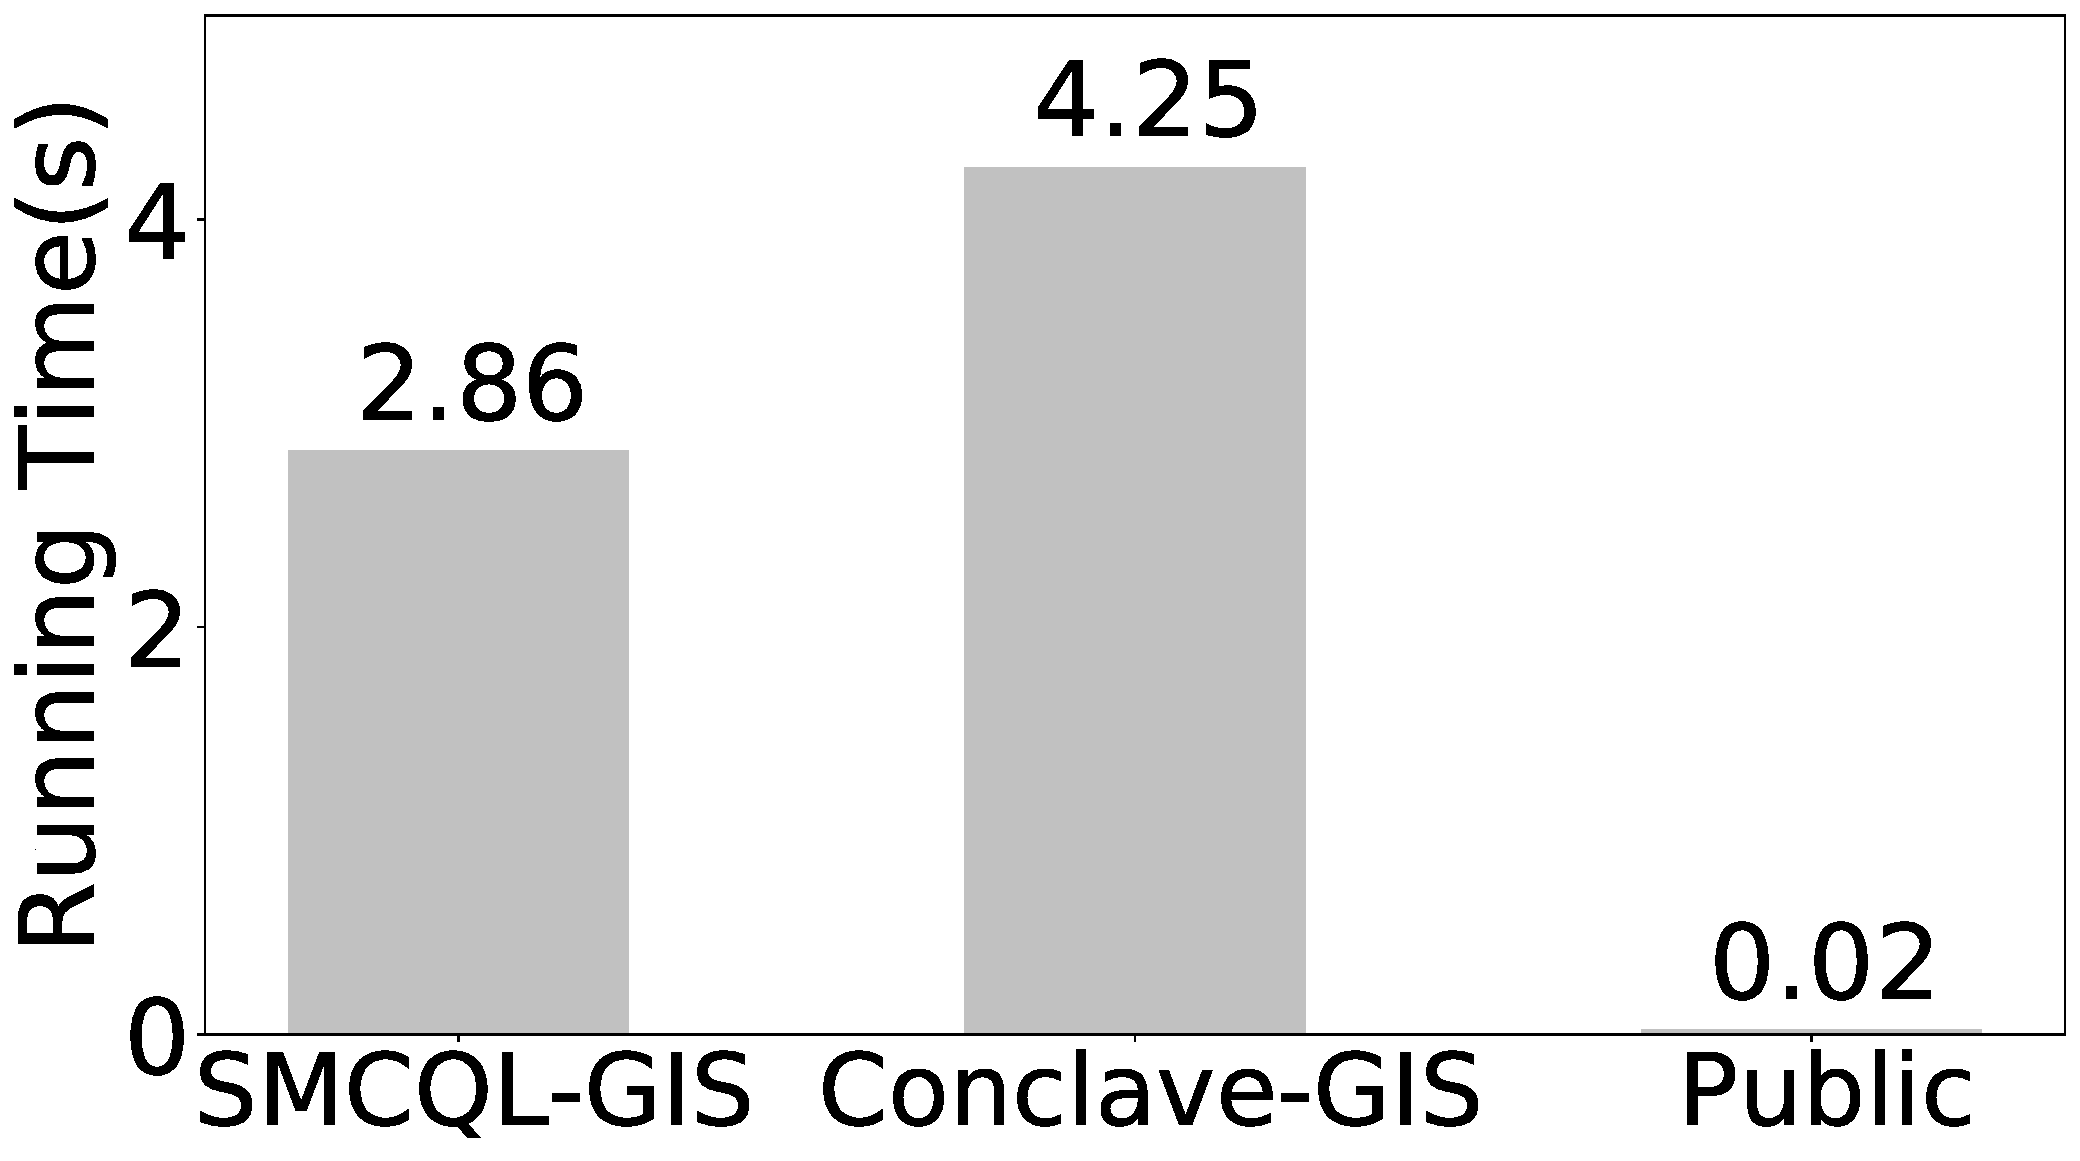
\includegraphics[width=\linewidth]{intro_time.pdf}
        \caption{Running time}
		\label{fig:cmp-runtime-k}
   \end{subfigure}
   \begin{subfigure}{0.242\textwidth}
        \centering
        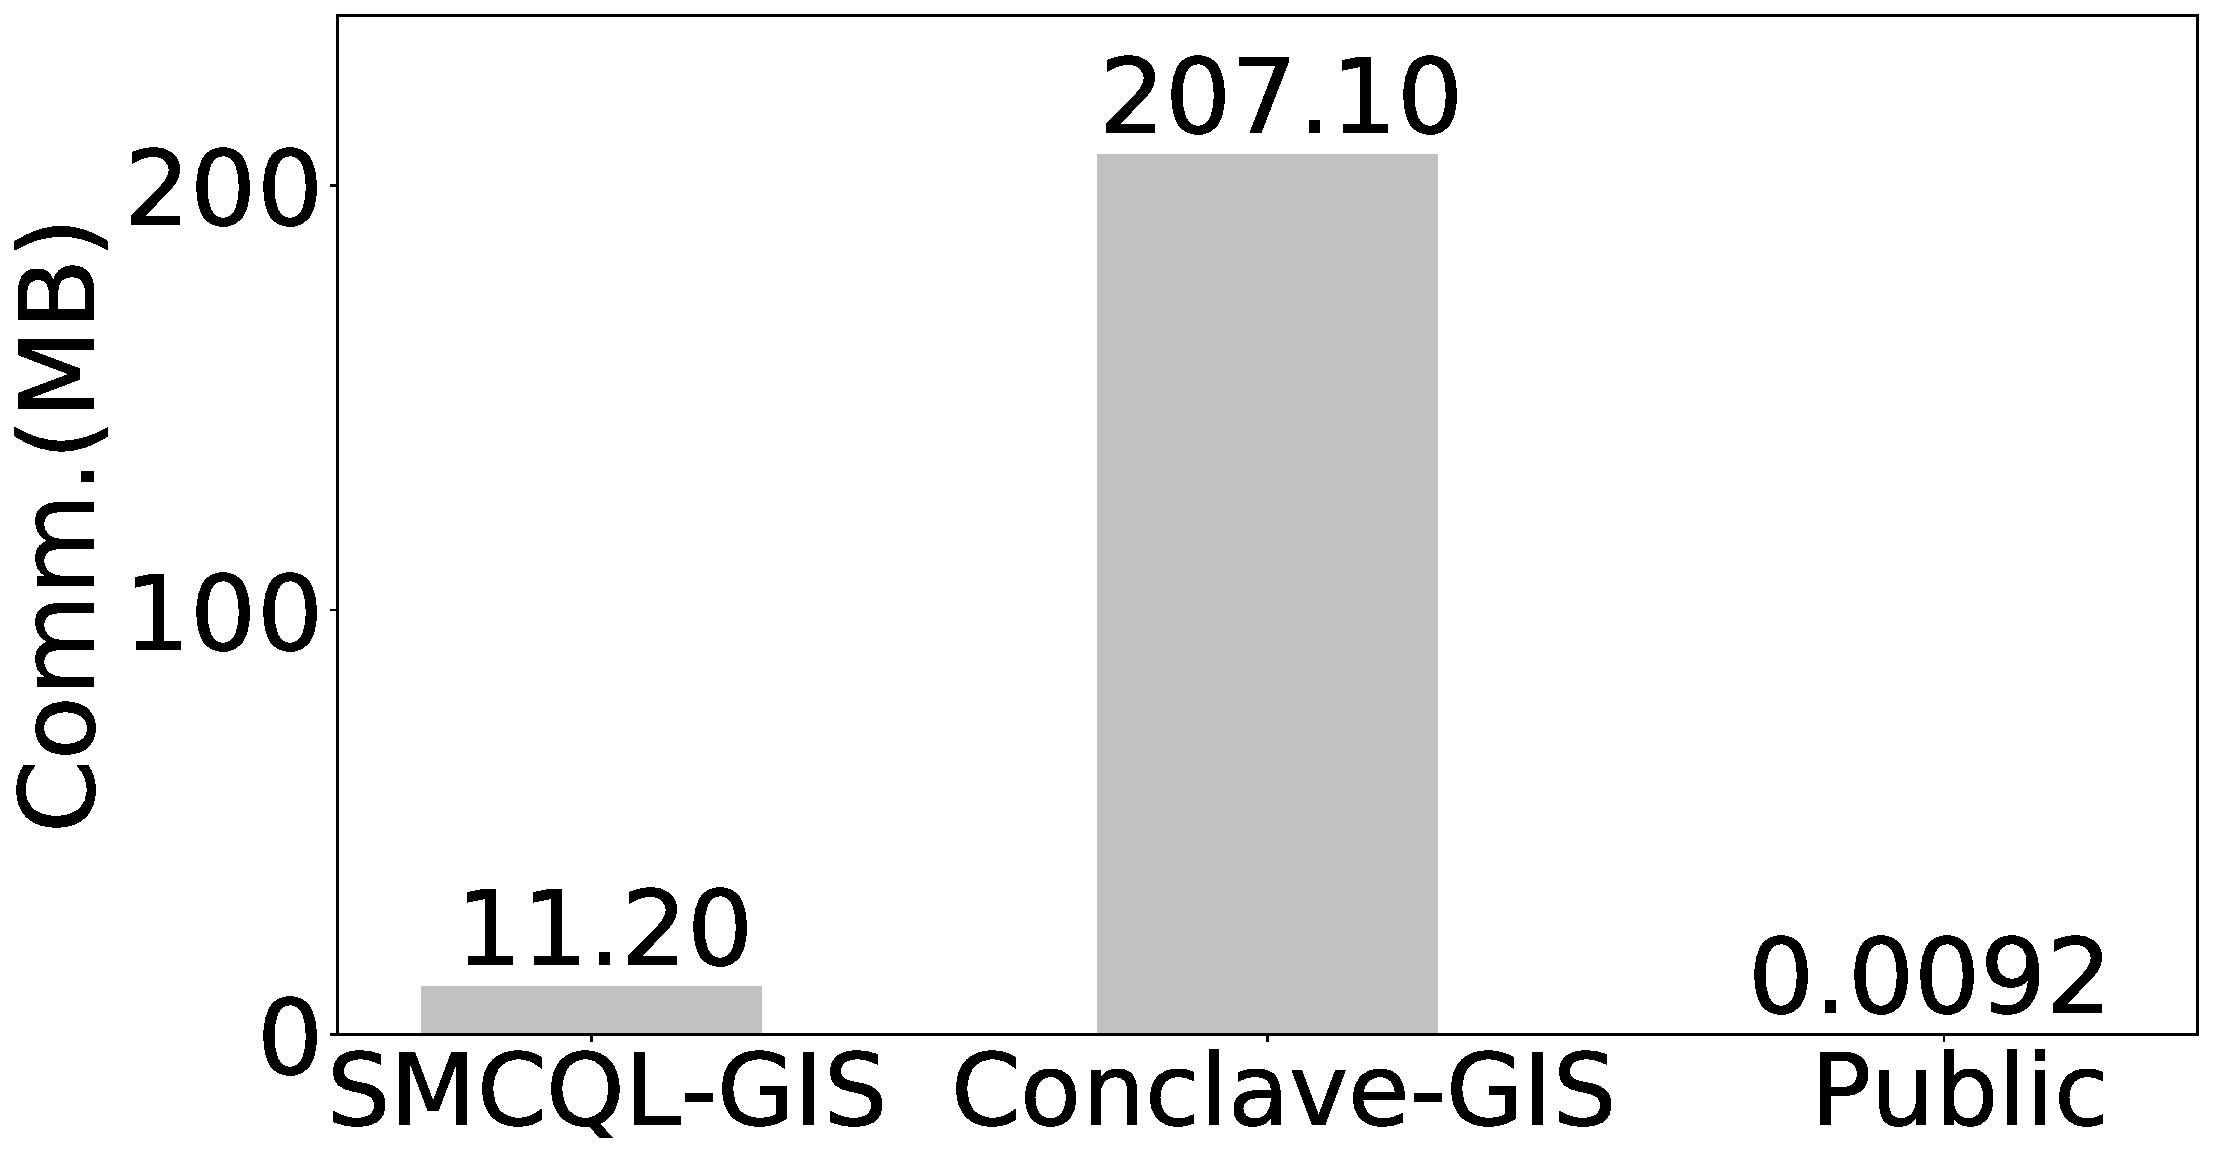
\includegraphics[width=\linewidth]{intro_cost.pdf}
        \caption{Communication cost}
		\label{fig:cmp-network-k}
    \end{subfigure}
    \caption{Inefficiency of \conclave and \smcql on asymmetric federated kNN query,
    where \smcql and \conclave are our extensions on SMCQL \cite{vldb17smcql} and Conclave \cite{eurosys19conclave} to spatial queries (see \secref{sec:experiment-setup}).}
    \label{fig:cmp-k}
\end{figure}

\subsubsection{Understanding the Efficiency Bottleneck}
\label{subsubsec:understanding}

Prior studies are inefficient on federated spatial queries for the following reasons.
\begin{itemize}
    \item \textbf{Excessive Secure Distance Operations}.
    When processing the test query, over $99\%$ time is spent on secure operations (\eg secure distance comparisons) as shown in \tabref{tab:breakdown}.
    Specifically, \smcql and \conclave adopt sorting to find kNNs among $nk$ candidates by using $O(nk \log(nk))$ secure distance comparisons.
    A single secure distance comparison in \smcql takes 209 ms, while in \conclave it takes 248 ms, which equals the time required for at least $10^6$ plaintext comparisons.
	
    \item \textbf{Reliance on General-Purpose Libraries.}
    Existing methods use general-purpose libraries to implement secure operations (\eg ObliVM~\cite{DBLP:conf/sp/LiuWNHS15} in SMCQL~\cite{vldb17smcql}). 
    General-purpose libraries sometimes sacrifice efficiency for generalization or compatibility.
    For example, the secure summation used in \sysname can be $16\times$ faster than that in ObliVM (see \secref{sec:evaluations}).
    As will be shown in \secref{sec:rewriter}, federated spatial queries can be processed with only a few secure operations.
    This facilitates acceleration by dedicated protocols specifically tailored for these secure operations.
\end{itemize}

\fakeparagraph{Takeaway}
Our study shows that existing secure query processing solutions (\eg \cite{vldb17smcql, eurosys19conclave}) for data federations are inefficient for spatial queries.
The inefficiency comes from \textit{(i)} massive secure distance operations, and is exacerbated by \textit{(ii)} adopting general-purpose libraries for these SMC operations.
In response, we propose \sysname, a solution with \textit{(i)} a novel execution plan for federated spatial queries that involve notably fewer secure operations 
(see \secref{sec:rewriter}) and \textit{(ii)} each secure operator can be implemented in high efficiency via dedicated methods (see \secref{sec:drivers}).
As next, we give an overview of \sysname and elaborate on its functional modules in the following.


\section{\sysname Overview}
\label{sec:overview}

\sysname is a solution that enables efficient and secure spatial queries over a data federation.
It addresses the inefficiency of federated spatial query processing via two modules:
\textit{(1)} a novel \textit{query rewriter} that decomposes federated spatial queries into \textit{plaintext and secure operators}, with the former executed within each silo and the latter across silos;
\textit{(2)} \textit{drivers} that implement these operators as \textit{plaintext and secure primitives} leveraging dedicated algorithms and optimizations.
\sysname also contains a transparent \textit{query interface} to support federated spatial queries written in native SQL.
We will briefly explain its architecture and workflow as follows.

\subsection{Architecture}
\label{sec:architecture}

\begin{figure}[t]
    \centering
    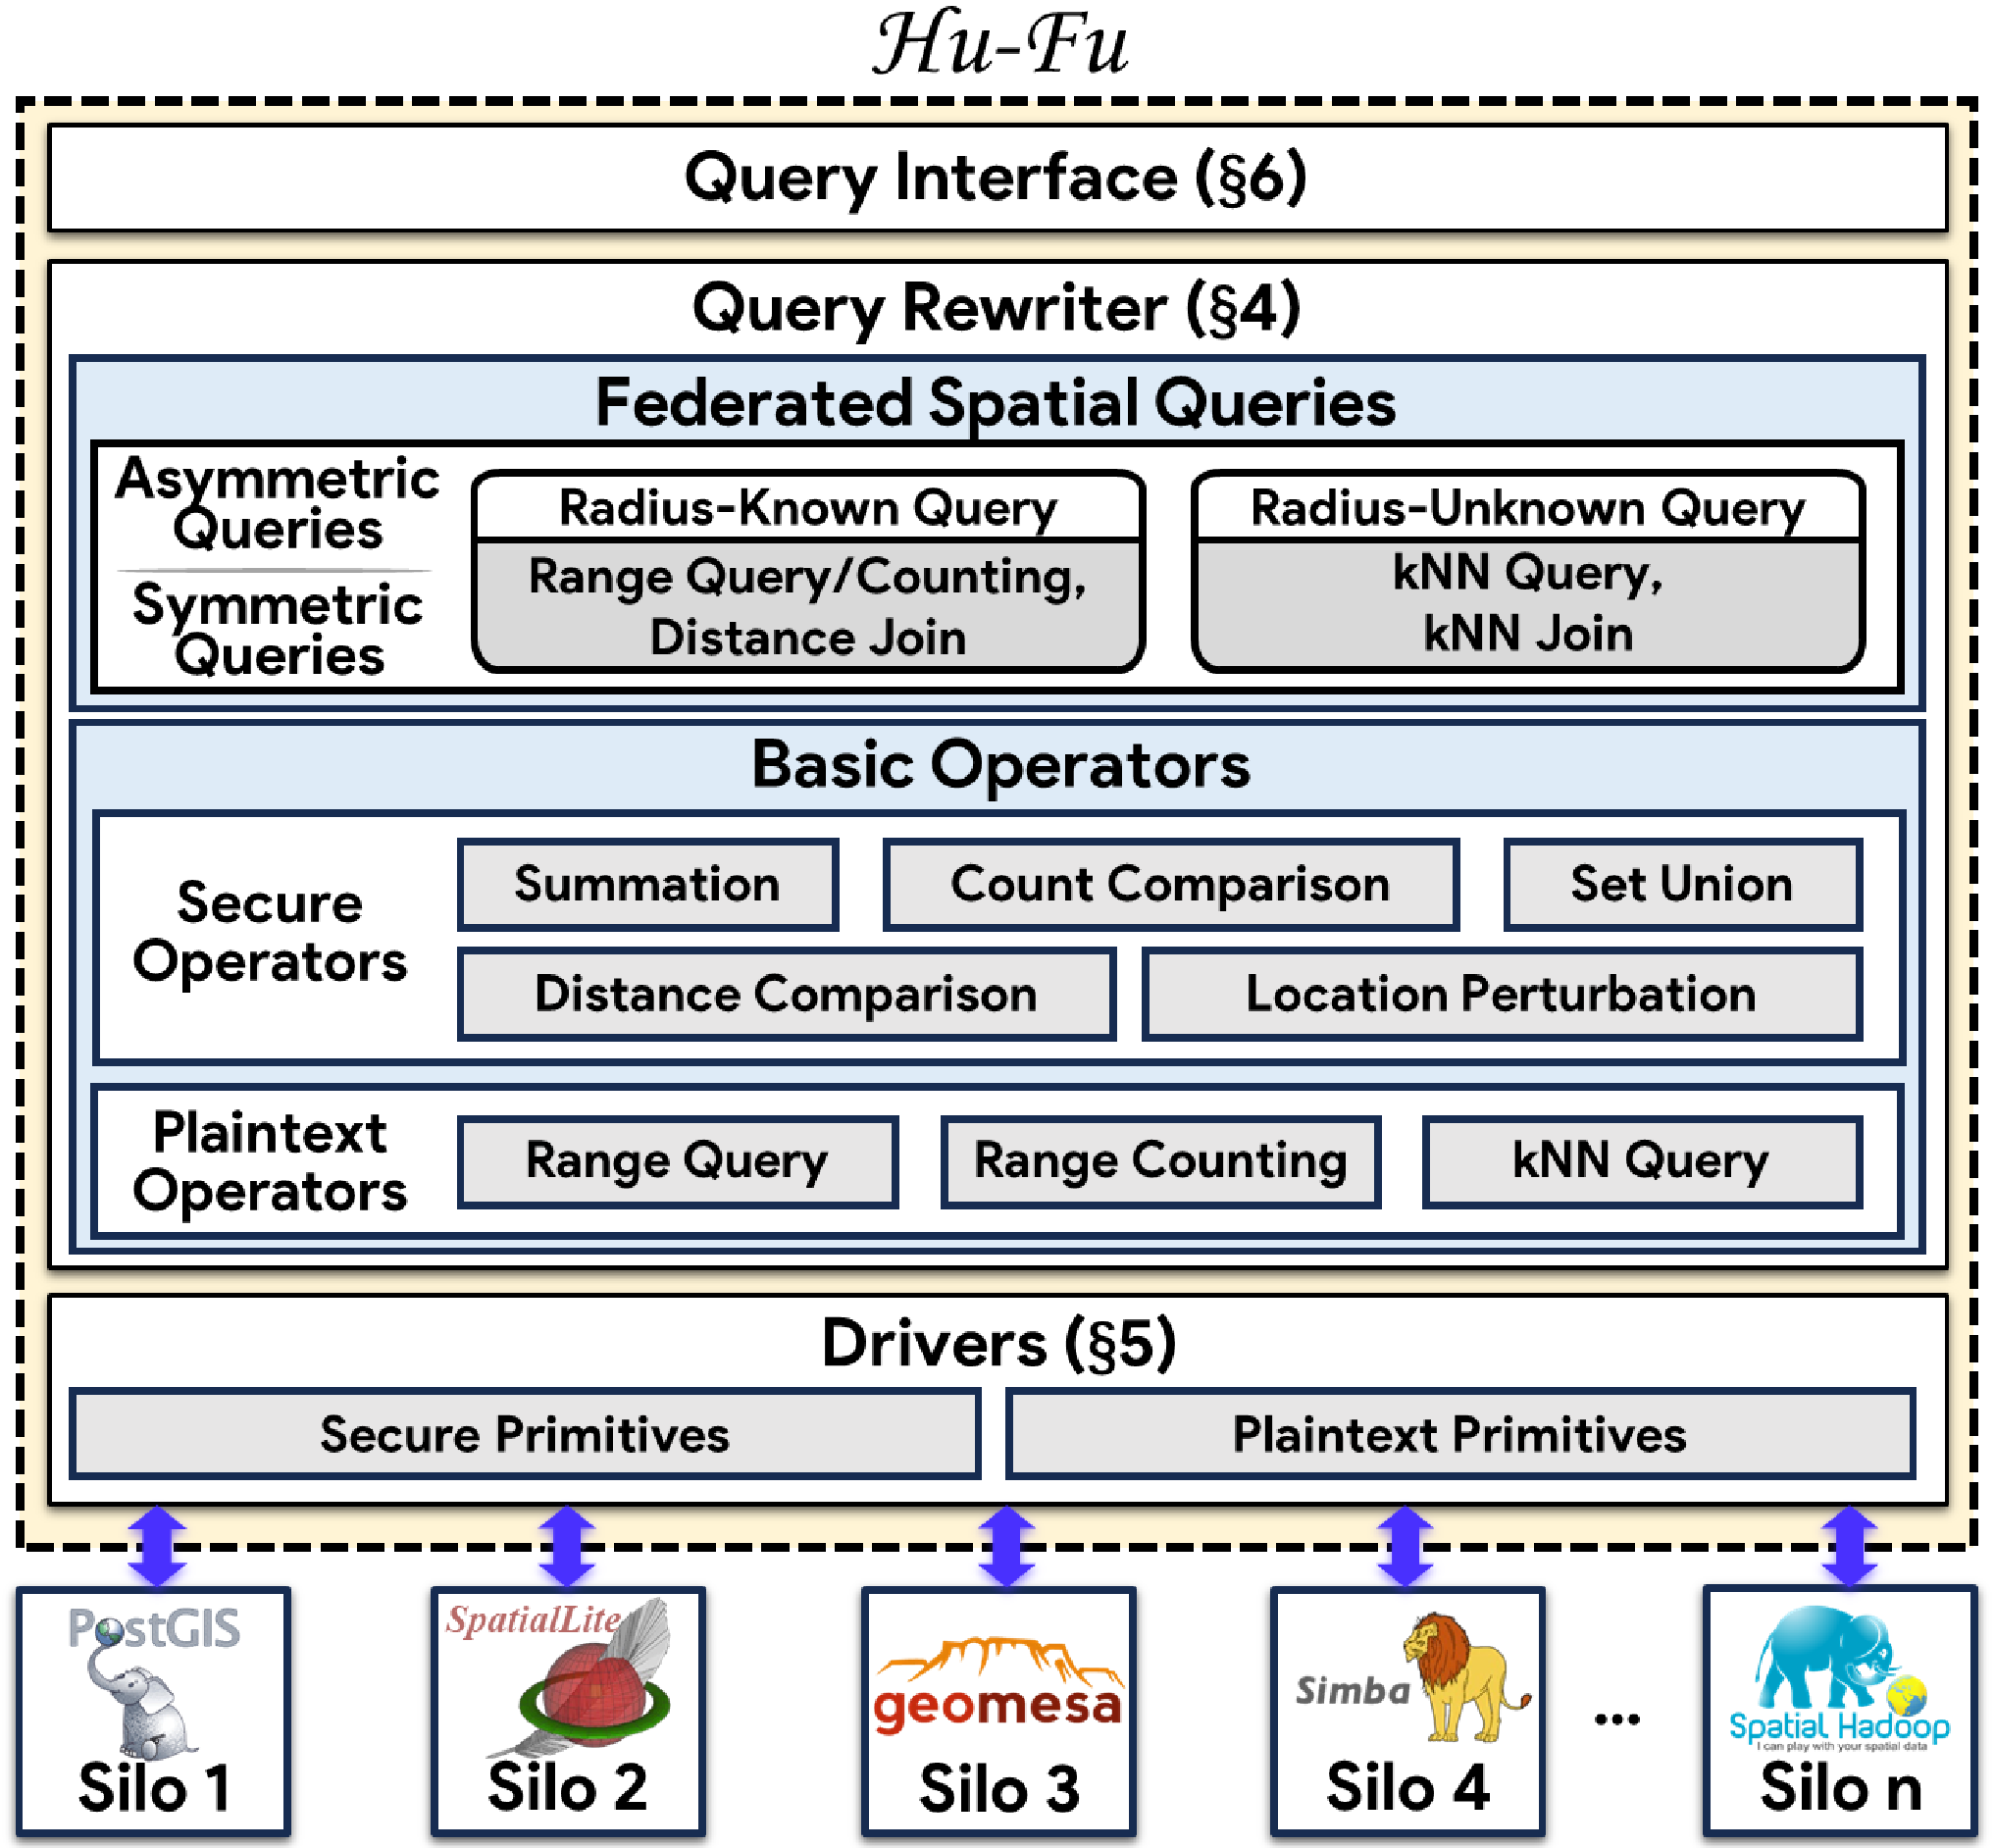
\includegraphics[width=0.46\textwidth]{hufu-new-architecture.pdf}
    \caption{Foundation architecture of \sysname.}
	\label{fig:arch}
\end{figure}

\figref{fig:arch} shows the architecture of \sysname, which consists of three modules: \textit{query rewriter}, \textit{drivers}, and \textit{query interface}.
From a functional perspective, the query rewriter and drivers optimize the query \textit{efficiency}, and the query interface improves the \textit{usability} of \sysname.

\fakeparagraph{Query Rewriter (\secref{sec:rewriter})}
It decomposes mainstream spatial queries (federated range query, range counting, kNN query, distance join, and kNN join) into plaintext operators (executed within silos) and secure operators (executed across silos).
We define three \textit{plaintext} operators (plaintext range query, range counting, and kNN query) and five \textit{secure} operators (secure summation, count comparison, set union, distance comparison, and location perturbation) as the basic operators. 
We also design novel execution plans that decompose these federated spatial queries into basic operators.

\fakeparagraph{Drivers (\secref{sec:drivers})} 
\sysname's drivers implement the basic operators defined in the query rewriter as efficient \textit{primitives} that can adapt to heterogeneous spatial databases at the backend.
Each operator is implemented by a specific primitive. 
Specifically, secure operators are implemented as \textit{secure primitives} with dedicated optimizations \cite{DBLP:journals/dke/EmekciSAA07, DBLP:conf/esorics/BogdanovLW08, DBLP:conf/socialcom/JurczykX11, DBLP:conf/edbt/KesarwaniKNPSMM18}. 
Plaintext operators are implemented as \textit{plaintext primitives} on top of the underlying spatial databases, which support various systems, \eg PostGIS~\cite{postgis}, SpatiaLite~\cite{spatialite}, MySQL~\cite{mysql}, GeoMesa~\cite{ds15geomesa}, Simba~\cite{sigmod16simba} and SpatialHadoop~\cite{icde15spatialhadoop}.

\fakeparagraph{Query Interface (\secref{sec:interface})}
This module \textit{(1)} provides a transparent and unified federation view to users, and \textit{(2)} supports both asymmetric and symmetric federated spatial queries written in SQL.
We implement the query interface by extending the schema manager and parser of Calcite \cite{DBLP:conf/sigmod/BegoliCHML18}.
We also provide interfaces such as JDBC for easy integration of \sysname to users' programs.

\begin{figure}[t]
    \centering
    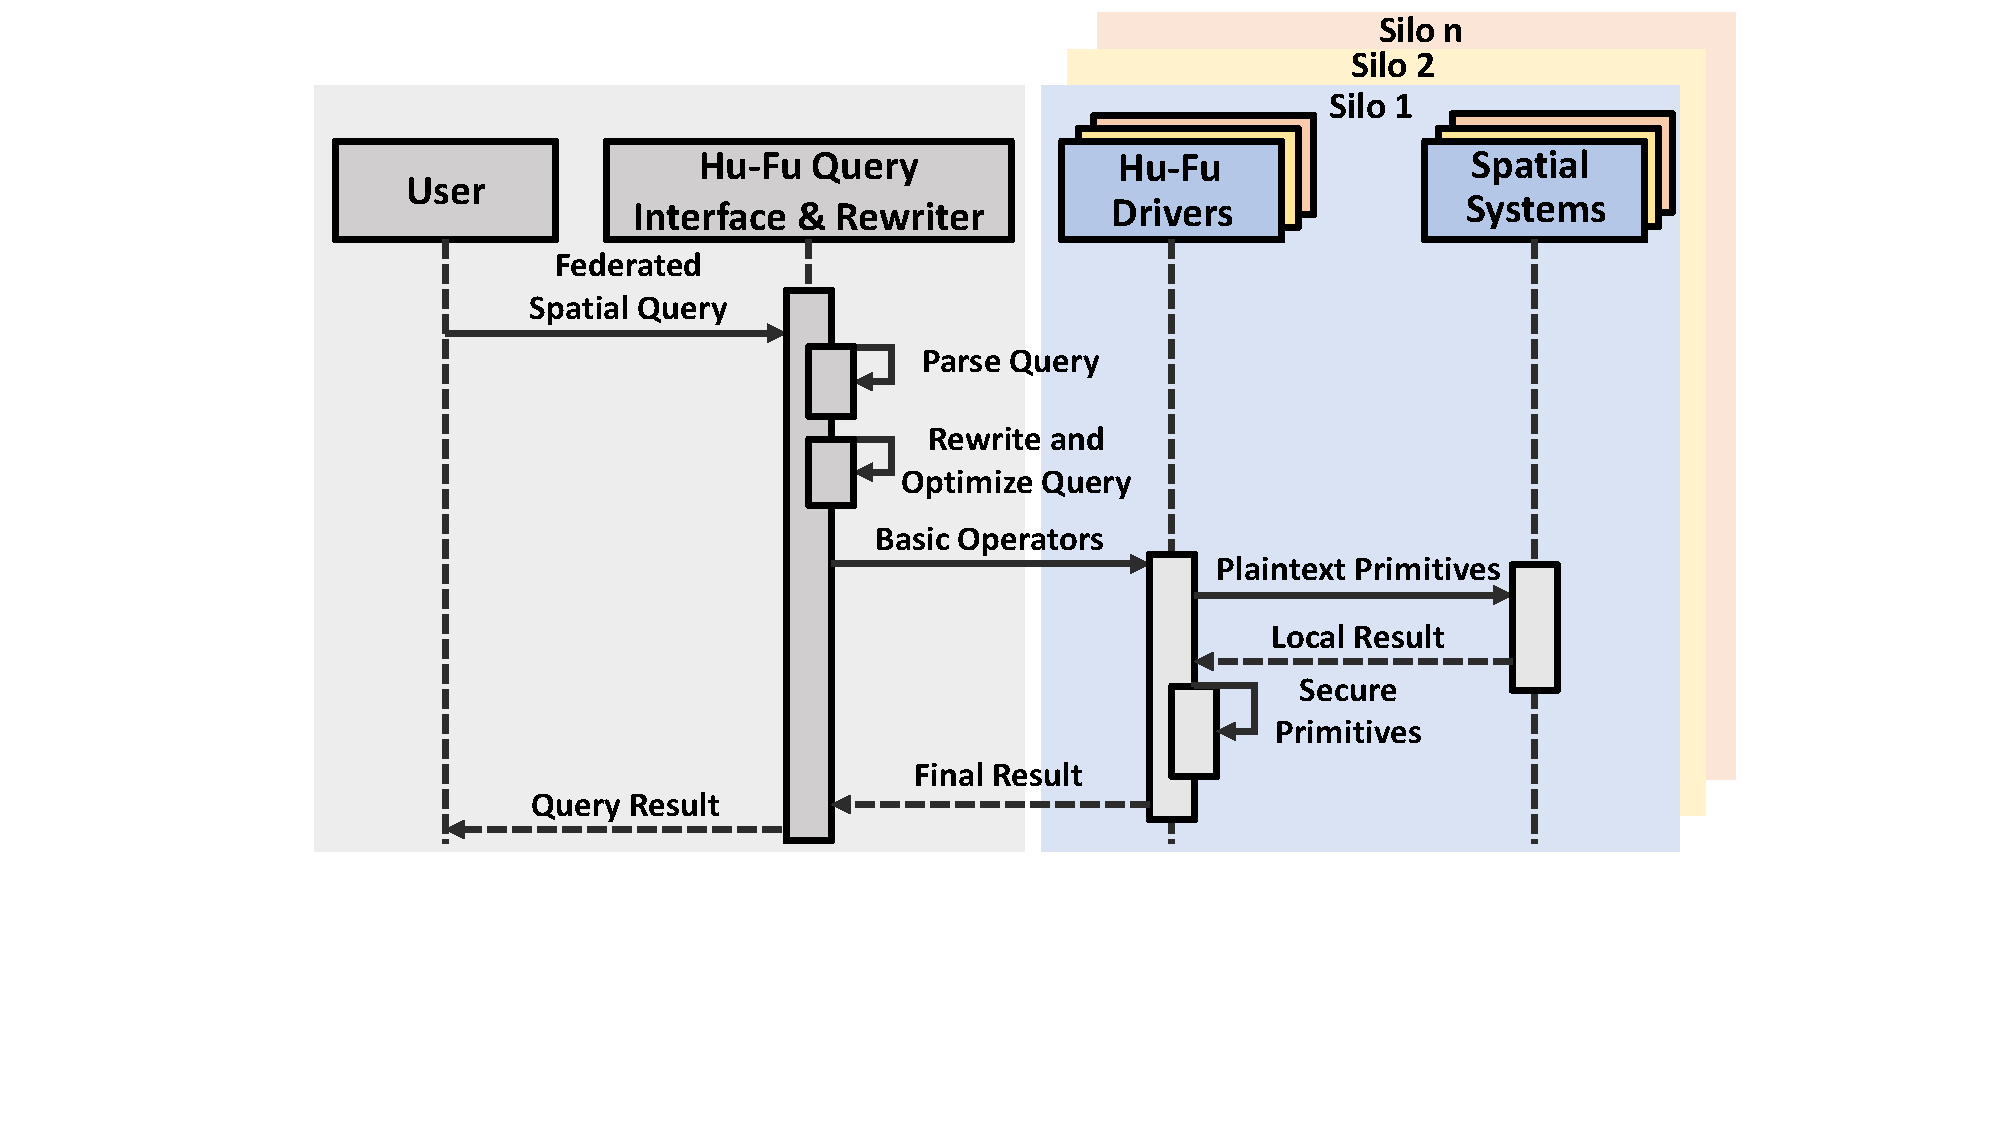
\includegraphics[width=0.46\textwidth]{hf-workflow.pdf}
    \caption{Illustration of \sysname workflow.}
	\label{fig:workflow}
\end{figure}

\subsection{Workflow}
\label{sec:workflow}

\figref{fig:workflow} depicts the workflow of \sysname for querying a data federation of $n$ silos.
The \textit{query interface} and \textit{query rewriter} are deployed on the user's machine to provide a portal for spatial services,
while each silo runs a \textit{driver} that interacts with its underlying spatial database.

In the workflow, a user's SQL-based federated spatial query is first parsed by the \textit{query interface}. 
Then, the \textit{query rewriter} transforms and optimizes the query into a sequence of plaintext and secure operators.
These operators are executed as primitives by the \textit{drivers}: plaintext primitives run locally on spatial databases to produce intermediate results,
while secure primitives assemble these partial results to obtain the final answer, which is returned to the user via the query interface.

\section{Query Rewriter}
\label{sec:rewriter}

This section presents the design of the query rewriter in \sysname, which decomposes a federated spatial query into basic operators to form the query execution plan.
Specifically, we first introduce the involved basic operators in \secref{sec:basic-operators}.
Next, we explain the overall decomposition strategies in \secref{sec:rewriter-framework}.
Then, we introduce the rewriter of \textit{asymmetric} federated spatial queries in \secref{sec:asymmetric} from two categories: \textit{radius-known} and \textit{radius-unknown} queries.
Since asymmetric federated spatial queries do not assume query privacy,
we also propose efficient solutions to \textit{symmetric} federated spatial queries in \secref{sec:symmetric}.
Finally, we discuss practical issues in \secref{sec:discussion}.

\subsection{Basic Operators}
\label{sec:basic-operators}

Our acceleration strategy is to \textit{decompose queries into basic operators so that the majority of distance-related operations occur within silos in plaintext}, thereby reducing the need for secure operations across silos.
The selection principle of basic operators is explained below.

\subsubsection{Operator Selection Principles}
\label{sec:basic-principles}

There are two categories of basic operators in \sysname: \textit{plaintext} and \textit{secure} operators. 
The \textit{plaintext} operators handle local queries within each individual silo, while the \textit{secure} operators perform atomic computations over sensitive data in a privacy-preserving manner.
\begin{itemize}
    \item \textbf{Plaintext Operators.} 
    They can involve the distance-related operations compulsory in spatial queries, but should be common operations widely supported by diverse spatial databases.
    
    \item \textbf{Secure Operators.} 
    They should avoid distance-related operations unless strictly necessary, and efficiently implemented operators are preferable.
\end{itemize}

Adhering to these principles, we select three plaintext operators and five secure operators, which will be elaborated in \secref{sec:in-silo} and \secref{sec:cross-silo}, respectively.

\subsubsection{Plaintext Operators}
\label{sec:in-silo}

We define three plaintext operators: \textit{plaintext range query, range counting, and kNN query}.
These operators are performed within each silo $F_i$.
Hence, they can be conducted in plaintext without compromising security. 

\begin{definition}[Plaintext Range Query/Counting]
\label{def:prq}
    Given a silo $F_i$ and a query range $\mathcal{R}$, the \textit{plaintext range query} $\lrq(F_i, \mathcal{R})$ retrieves the spatial objects in $F_i$ that fall within $\mathcal{R}$, 
    and the \textit{plaintext range counting} $\lrc(F_i, \mathcal{R})$ returns the number of such objects.
\end{definition}

\begin{definition}[Plaintext kNN Query]
\label{def:pknn}
    Given a silo $F_i$, a query object $q$, and a positive integer $k$, the \textit{plaintext kNN query} $\knn(F_i, q, k)$ retrieves the k nearest spatial objects in $F_i$ to the query object $q$.
\end{definition}

The plaintext operators comply with the principles described in \secref{sec:basic-principles}, because they are supported by almost all spatial databases.
They are implemented as \textit{plaintext primitives} in \sysname drivers, which we defer to \secref{sec:plaintext-primitives}.
The query range can be various shapes, such as circles and rectangles. 
For ease of presentation, we mainly focus on circular ranges in this section and discuss extensions to other shapes in \secref{sec:discussion}.

\subsubsection{Secure Operators}
\label{sec:cross-silo}

We define five secure operators: \textit{summation, count comparison, set union, distance comparison, and location perturbation}. The first three secure operators are designed to preserve data privacy, while the latter two secure operators aim to protect query privacy.

\begin{definition}[Secure Summation]
\label{def:ssum}
Given $n$ data silos $\{F_i\}$ each holding a private value $v_i$, this operator $\ssum$ sums up these values, \ie $\ssum(v_1,\cdots,v_n) = \sum_{i=1}^n{v_i}$,
while protecting the privacy of $v_i$ in silo $F_i$ from all other silos $F_j$ ($\forall j \neq i$).
\end{definition}

\begin{definition}[Secure Count Comparison]
\label{def:scmp}
Given $n$ data silos $\{F_i\}$ each holding a private count $v_i$ and a public constant $k$, this operator $\scmp$ compares the sum of these counts with $k$, \ie $\scmp(v_1,\cdots,v_n,k) = sign(\sum_{i=1}^n{v_i}-k)$, without leaking the sum $\sum_{i=1}^n{v_i}$ or the count $v_i$ in silo $F_i$ to any other silos $F_j$ ($\forall j \neq i$).
\end{definition}

\begin{definition}[Secure Set Union]
\label{def:ssun}
Given $n$ data silos $\{F_i\}$ each holding a set of spatial objects $S_i=\{o^i_{1}, \cdots, o^i_{{m_i}}\}$, this operator $\ssun$ computes the union of spatial objects from all silos,
\ie $\ssun(S_1,\cdots,S_n) = \cup_{i=1}^{n}S_i$,
without leaking the spatial objects $S_i$ in silo $F_i$ to any other silos $F_j$ ($\forall j \neq i$).
\end{definition}

\begin{definition}[Secure Distance Comparison]
\label{def:sdcmp}
Given a query user holding a private location $l_q$, a data silo holding a private location $l_o$, and a distance threshold $r$,
this operator $\sdcmp$ compares the distance between $l_q$ and $l_o$ with the threshold $r$,
\ie $\sdcmp(l_q,l_o,r) = sign(\dist(l_q,l_o)-r)$, 
without leaking the location of either party (\ie the user or silo) to the other.
\end{definition}

\begin{definition}[Secure Location Perturbation]
\label{def:sdp}
Given a private location $x \in \mathbb{R}^2$, this operator $\geoi$ obfuscates it into a location $z = \geoi(x)$ 
while satisfying $(\epsilon,\delta)$-Geo-Indistinguishability (Geo-I) \cite{DBLP:journals/corr/abs-2312-12012}.
The privacy requirement of $(\epsilon,\delta)$-Geo-I is satisfied iff the following inequality holds for any two locations $x, x'$ in the location set and any location subset $Z$:
\begin{equation}
    \Prob[\geoi(x)\in Z] \le e^{\epsilon \dist(x,x')} \cdot \Prob[\geoi(x')\in Z] + \delta
\end{equation}
where $\Prob[\geoi(x)\in Z]$ is the probability that the perturbed location belongs to the subset $Z$,
and $\epsilon,\delta$ represent the privacy preservation level of Geo-I.
\end{definition}

$\epsilon$-Geo-I \cite{DBLP:conf/ccs/AndresBCP13} adapts the de facto standard privacy notion, \textit{differential privacy} \cite{DBLP:series/synthesis/2016Li}, to protect location data, where $\epsilon$ is known as the privacy budget.
$(\epsilon,\delta)$-Geo-I relaxes the definition of $\epsilon$-Geo-I by allowing a small failure probability $\delta$. This way of relaxation has gained widespread usages in (standard) differential privacy \cite{DBLP:series/synthesis/2016Li}.

\fakeparagraph{Remark}
The secure operators comply with the principles in \secref{sec:basic-principles} since \textit{(1)} most of them do not involve distance operations (with the exception of secure distance comparison) and \textit{(2)} all of them have dedicated and efficient implementations (see \secref{sec:secure-primitives} for details).

\subsection{Overview of Our Decomposition Strategies}
\label{sec:rewriter-framework}

In the following, we formally define the federated spatial queries and introduce our taxonomy to categorize them (\secref{sec:rewriter-framework-taxonomy}).
We then elaborate on the main ideas of our decomposition strategies for each category (\secref{sec:rewriter-framework-idea}).

\subsubsection{Federated Spatial Queries and Taxonomy}\label{sec:rewriter-framework-taxonomy}

Before diving into our decomposition strategies, we first define the five federated spatial queries.
The privacy requirement below includes either data privacy alone or both data and query privacy defined in \secref{subsec:problem}.

\begin{definition}[Federated Range Query/Counting]\label{def:range}
Given a federation $F$ of $n$ data silos $\{F_i\}$, and a query range $\mathcal{R}$, a \textit{federated range query} retrieves all spatial objects located within $\mathcal{R}$, while a \textit{federated range counting} returns the number of such objects. 
Both queries need to satisfy the privacy requirement.
\end{definition}

\begin{definition}[Federated Distance Join]\label{def:disjoin}
Given a federation $F$ of $n$ data silos $\{F_i\}$, an input dataset $Q$ of spatial objects, and a distance radius $r$, a federated distance join retrieves all pairs of objects $(q,o)$ where $q \in Q, o \in F$ such that the distance $\dist(l_q, l_o) \le r$, while satisfying the privacy requirement, \ie
\begin{equation*}
Q \bowtie_{r} F = \{(q,o)\ |\ q \in Q, o \in F, \dist(l_q, l_o) \le r\}.
\end{equation*}
\end{definition}

\begin{definition}[Federated kNN Query/Join]\label{def:knn}
Given a federation $F$ of $n$ data silos $\{F_i\}$, a query object $q$, and a positive integer $k$, a \textit{federated kNN query} retrieves the $k$ nearest objects in $F$ to the query object $q$, \ie
\begin{equation*}
    \forall o \in \text{kNN}(q), \forall o' \in F \setminus \text{kNN}(q), \dist(q, o) \le \dist(q, o').
\end{equation*}
When the query objects form an input dataset $Q$, a \textit{federated kNN join} retrieves all pairs of objects $(q,o)$ where $q \in Q$ and $o$ belongs to the kNN of $q$ in $F$, \ie
\begin{equation*}
    Q \bowtie_\text{kNN} F = \{(q,o)\ |\ q \in Q, o \in \text{kNN}(q)\}.
\end{equation*}
Both queries need to satisfy the privacy requirement.
\end{definition}

\fakeparagraph{Taxonomy}
The above queries can be categorized from \textit{two orthogonal dimensions}: 
the scope of the privacy requirement and whether the searching radius (of the query range) is explicitly given.
Specifically, based on whether query privacy is included in the privacy requirement, the queries are classified into \textit{asymmetric} and \textit{symmetric} queries (see the differences in \secref{subsec:problem}).
Based on whether the searching radius is explicitly given, the queries are classified into \textit{radius-known} and \textit{radius-unknown} queries.
Intuitively, the federated range query, range counting, and distance join belong to radius-known queries, while the federated kNN query and kNN join belong to radius-unknown queries.

\subsubsection{Main Idea of Our Decomposition Strategies}\label{sec:rewriter-framework-idea}

\fakeparagraph{Basic Principle}
In \sysname, the core principle of the query rewriter is to decompose federated spatial queries into as many plaintext operators and as few secure operators as possible such that a large portion of the query can be executed in plaintext without compromising security.
At a high level, a federated spatial query is initially processed using plaintext operators within each silo, and their results are then securely assembled to form the final outcome.
At the minimum, one secure operator is compulsory, and additional secure operators may be required if there are interactions across silos.

Based on the aforementioned basic operators and taxonomy of queries, we now introduce the \textit{main ideas} of decomposing different categories of queries.

\fakeparagraph{Main Idea for Asymmetric Queries with Data Privacy Solely}
Our idea is elaborated as follows:
\begin{itemize}
    \item \textbf{Radius-Known Queries.}
    A radius-known query (\eg federated range query and range counting) can be decomposed into the corresponding plaintext operators within each silo and only one secure operator (\eg a secure set union or a secure summation) for assembling the partial results across silos.

    \item \textbf{Radius-Unknown Queries.}
    Each radius-unknown query (\eg federated kNN query) is viewed as an iterative process of trialing different search radii until exactly $k$ spatial objects are found within the circular search area.
    This execution can be converted into multiple radius-known queries (\eg federated range counting), with the number of radius-known queries minimized by a binary search.
    Each iteration utilizes a secure operator to ensure data privacy.
\end{itemize}

\fakeparagraph{Key Insight for Symmetric Queries with Both Data and Query Privacy}
When additionally considering query privacy, our key insights are as follows:
\begin{itemize}
    \item \textbf{Radius-Known Queries.}
    A native solution employs a secure distance comparison operator for every spatial object, but leads to excessive secure distance operations.
    Instead, we first obfuscate the sensitive query location using a secure location perturbation operator to create a noised location that can be safely published to each silo. 
    Then, leveraging the previous idea for radius-known queries, each silo identifies a small set of candidates. 
    For each candidate, a secure distance comparison operator verifies if its distance to the query location is within the specified radius, while protecting query privacy.
    
    \item \textbf{Radius-Unknown Queries.}
    Similar to the aforementioned ideas for decomposing radius-unknown queries, we can still decompose them into a series of radius-known queries.
\end{itemize}

\subsection{Decomposing Asymmetric Queries with Data Privacy Only}
\label{sec:asymmetric}

This subsection proposes our methods for decomposing radius-known queries (\secref{sec:asymmetric-krad}) and radius-unknown queries (\secref{sec:asymmetric-urad}), which only consider data privacy.
The decomposition plans are summarized in \tabref{tab:rewriter}.

\begin{table*}[t]
\centering
\caption{The number of basic operators in the decomposition plans of \textit{asymmetric} federated spatial queries. Radius-known queries only involve one type of secure operators (secure summation or set union). Radius-unknown queries are executed in multiple rounds which additionally require secure count comparisons to ensure security.}
\label{tab:rewriter}
\begin{threeparttable}
\begin{small}
\begin{tabular}{llllll}
\toprule
\multirow{2}{*}{Category} & \multirow{2}{*}{\makecell[c]{Federated\\Spatial Query}} & \multicolumn{2}{c}{\#(Plaintext Operator)} & \multicolumn{2}{c}{\#(Secure Operator)}\\
\cmidrule(lr){3-4} \cmidrule(lr){5-6}
& & Range Query & Range Counting & Count Comparison & Set Union/Summation \\
\midrule
\multirow{3}{*}{Radius-Known} & Range Query     & $n$     & $0$   & $0$   & $1/0$ \\
& Range Counting  & $0$     & $n$   & $0$   & $0/1$ \\
& Distance Join   & $n|R|$  & $0$   & $0$   & $|R|/0$ \\
\midrule
\multirow{2}{*}{Radius-Unknown} & kNN Query & $n$ & $O(n\log{U})$  & $O(\log{U})$   & $1/0$ \\
& kNN Join        & $n|R|$ & $O(n|R|\log{U})$ & $O(|R|\log{U})$ & $|R|/0$           \\
\bottomrule
\end{tabular}
\end{small}
\begin{tablenotes}
	\item $n$ is the number of silos, $R$ is the input dataset in spatial joins, and $U$ is the upper bound for the binary-search radius.
\end{tablenotes}
\end{threeparttable}
\end{table*}

\subsubsection{Decomposing Radius-Known Queries}
\label{sec:asymmetric-krad}
Among the five queries, the federated range query, range counting, and distance join are radius-known queries. 

\fakeparagraph{Decomposition Plan}
(1) \textbf{Federated range query} can be decomposed into $n$ \textit{plaintext range queries}, each with a radius $r$, where each plaintext operator retrieves the partial result within each one of the $n$ silos.
Afterwards, a \textit{secure set union} operator assembles these partial result while maintaining data privacy.
(2) Similarly, \textbf{federated range counting} can be decomposed into $n$ \textit{plaintext range counting} operators to obtain $n$ partial counts.
These partial counts will later be aggregated by a \textit{secure summation} operator.
(3) \textbf{Federated distance join} is equivalent to requesting federated range queries $|R|$ times, each of which follows the previous plan.

\fakeparagraph{Complexity Analysis}
Let $\TRQ$ and $\TRC$ denote the time complexity of plaintext range query and range counting, respectively. 
$|S|$ denotes the size of returned set.
Based on the complexities of secure operators (see \secref{sec:secure-primitives}), the time complexity and communication cost of the radius-known queries are as follows.
(1) \textit{Federated range query} takes $O(\TRQ+n+|S|)$ time and $O(n+|S|)$ communication cost.
(2) \textit{Federated range counting} takes $O(\TRC+n^3)$ time and $O(n^2)$ communication cost.
(3) \textit{Federated distance join} takes $O(|R| \cdot \TRQ+n+|S|)$ time and $O(n+|S|)$ communication cost.

\subsubsection{Decomposing Radius-Unknown Queries}
\label{sec:asymmetric-urad}
Federated kNN query and kNN join are classified as radius-unknown queries due to the absence of an explicitly given range.
Their decomposition plan is to first get an appropriate range and then filter the points in the range, as explained in detail below.

\fakeparagraph{Decomposition Plan}
Similar to the relation between federated range query and federated distance join in \secref{sec:asymmetric-krad}, federated kNN join can be viewed as $|R|$ independent federated kNN queries.
Hence, we mainly explain how to decompose a federated kNN query.
\begin{itemize}
    \item \textbf{Basic Idea.}
    Recall from \secref{sec:rewriter-framework}, the strategy to decompose radius-unknown queries is to convert them into multiple rounds of radius-known queries.
    We first derive a radius $\thres$ via a binary search and then retrieve the spatial objects within this search range.
    For each radius $\thres$, we securely check whether the counting result is smaller than $k$.
    As long as $\thres$ falls between the $k$th and the $(k+1)$th nearest distance to the query object $q$, the spatial objects within this range are precisely  the $k$ nearest neighbors.

    \item \textbf{Algorithm Details.}
    \algref{alg:knn} illustrates the decomposition of a federated kNN query.
    Lines 1-8 derive the radius $r$.
    We initialize a lower bound ($l=0$) and upper bound ($u=U$) of the radius, where $U$ can be set as the spatial area's diameter or a user-defined value.
    A binary search is then performed to find the appropriate radius until reaching the \rev{distance precision $\epsilon_0$} (lines 2-9).
    In each iteration, $\thres$ is set to $(l+u)/2$.
    For each $\thres$, a \textit{plaintext range counting} operator is executed within each silo, and a \textit{secure count comparison} operator is invoked to compare the total count with the integer $k$ (lines 4-5).
    If the total count is less than $k$ (\ie $sign < 0$), indicating an undersized radius, $l$ will be increased to $\thres$.
    Conversely, if the total count exceeds $k$ (\ie $sign > 0$), $u$ will be decreased to $\thres$.
    The binary search ensures that the final radius $\thres$ is sufficiently close to the $k$th nearest distance.
    Finally, a \textit{plaintext range query} is executed on each silo, and the partial results are collected using a \textit{secure set union} (lines 9-10).
\end{itemize}

\rev{In \algref{alg:knn}, the distance precision $\epsilon_0$ is initially set based on the application requirement.
For example, many spatial applications (\eg taxi-calling) have a minimum distance precision requirement that is typically measured in meters.  
Then, $\epsilon_0$ can be set to 1 meter.}

\fakeparagraph{Complexity Analysis}
\algref{alg:knn} requires $O(\log \frac{U}{\epsilon_0}) = O(\log{U})$ iterations to obtain the final radius, where $\epsilon_0$ is a constant to denote this radius's precision.
In each iteration, the plaintext range counting takes $O(\TRC)$ time, and the secure count comparison takes $O(n)$ time and $O(n^2)$ communication cost.
In lines 9-10, \algref{alg:knn} performs a plaintext range query that takes $O(\TRQ)$ time and a secure set union that takes $O(n+k)$ time and $O(n+k)$ communication cost.
Overall, the total time complexity is $O((\TRC+n)\cdot\log{U} + \TRQ + k)$, and the communication cost is $O(n^2\cdot\log{U} + k)$.
Intuitively, the complexity of federated kNN join is equal to that of federated kNN query, multiplied by a factor $|R|$.

\setlength{\textfloatsep}{1ex}
\setlength{\floatsep}{1ex}
\begin{algorithm}[t]
	\caption{\small{Asymmetric federated kNN query}}\label{alg:knn}
	\KwIn{federation $F$, query object $q$, integer $k$}
	\KwOut{the (exact) query answer $ans$}
    $[l,u] \gets [0,U]$, where $U$ is a predefined upper bound\;
    \While {$u - l \geq \epsilon_0$} {
        $\thres \leftarrow (l+u)/2$, $\mathcal{R} \gets \text{circle}(q, \thres)$\;
        \ForEach(\rev{// perform in parallel}){\rev{silo $F_i \in F$}}{
            $v_i \gets$ plaintext range counting $\lrc(F_i, \mathcal{R})$\; 
        } 
        $sign \gets$ secure count comparison $\scmp(\{v_i\}, k)$\;
        \textbf{if} $sign < 0$ \textbf{then} $l \leftarrow \thres$\;
        \textbf{else if} $sign > 0$ \textbf{then} $u \leftarrow \thres$\;
        \textbf{else} \textbf{break}\;
    }
    \ForEach(\rev{// perform in parallel}){\rev{silo $F_i \in F$}}{
        $S_i \gets$ plaintext range query $\lrq(F_i, \text{circle}(q, \thres))$\;
    }
    \KwRet{$ans$} $\gets$ secure set union $\ssun(S_1,\cdots,S_n)$\;
\end{algorithm}
\afterpage{\global\setlength{\textfloatsep}{\oldtextfloatsep}}
\afterpage{\global\setlength{\floatsep}{\oldfloatsep}}

\begin{figure*}[t]
    \centering
    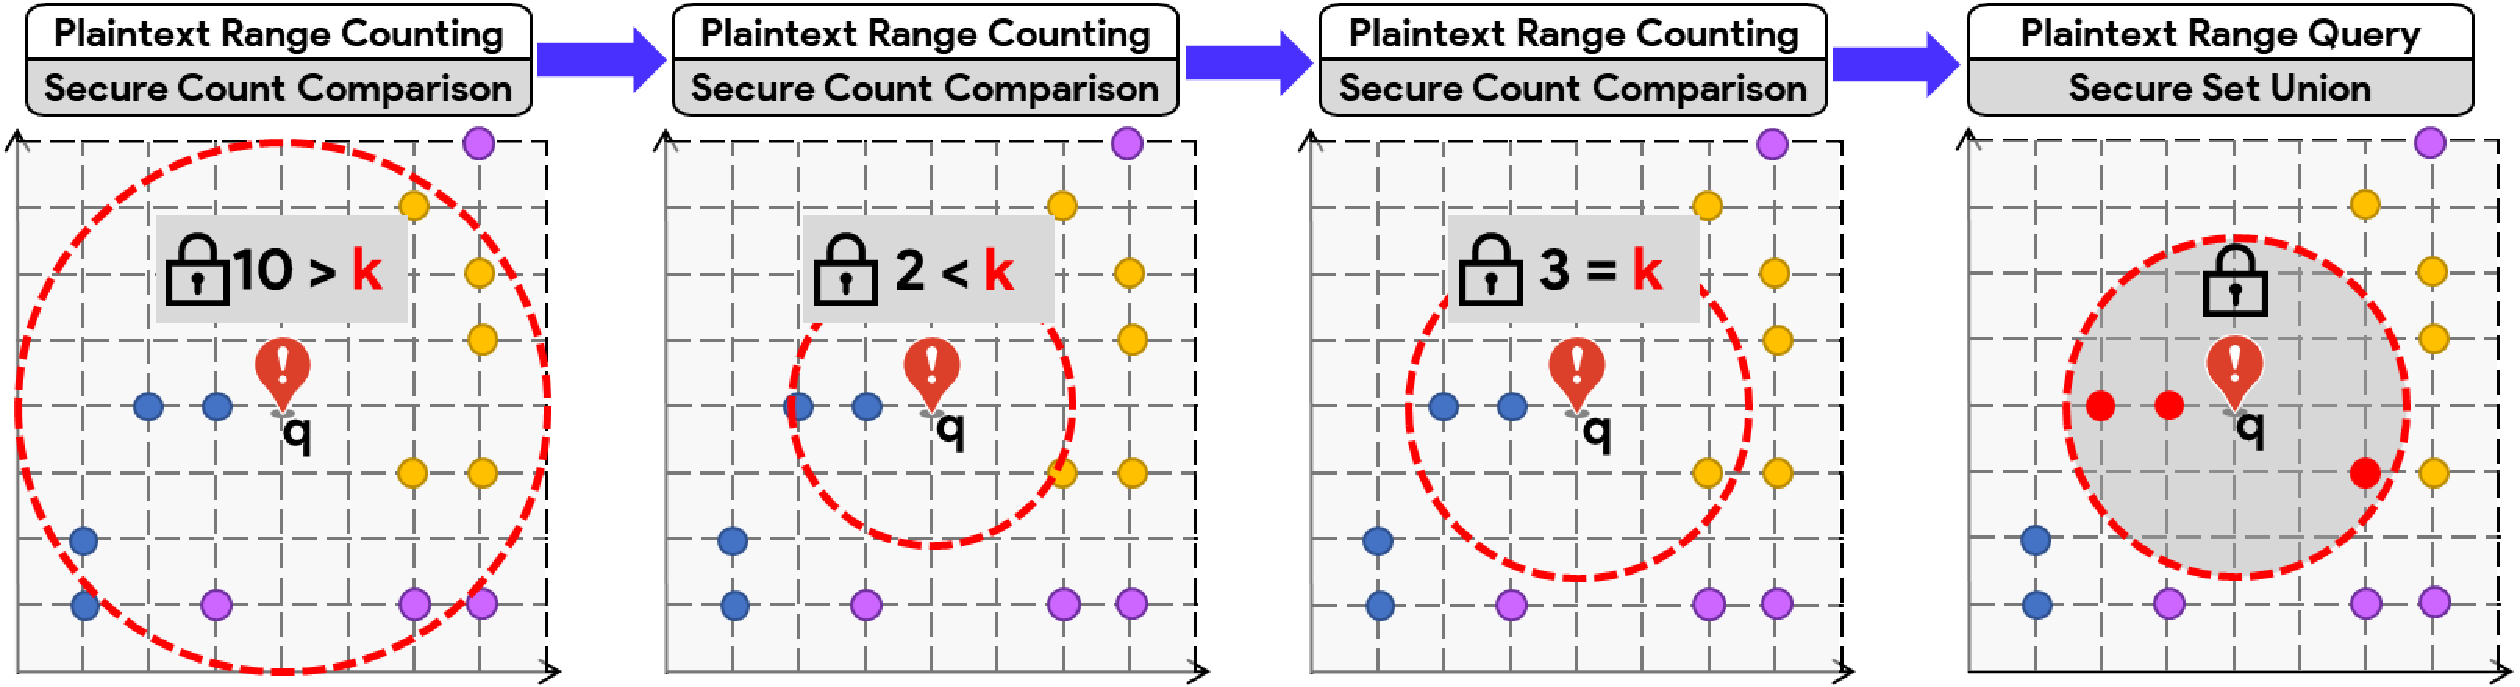
\includegraphics[width=0.94\textwidth]{fed-knn-example.pdf}
	\caption{Running example for (asymmetric) federated kNN query ($k=3$).}
	\label{fig:knn}
\end{figure*}

\begin{example}
\figref{fig:knn} illustrates the procedure of \algref{alg:knn} with a query point $(4,4)$ and $k = 3$ over 3 silos,
where the objects with the same color belong to the same silo.
The query rewriter decomposes this query into multiple rounds of radius-known queries.
In the 1st round, a plaintext range counting with center $(4,4)$ and radius $4$ is sent to each silo and a secure count comparison with $k$ is performed across silos.
And we get $10$ objects, which is greater than $k$.
Hence in the 2nd round, the radius decreases to $2$ and is sent to each silo for plaintext range counting and secure count comparison.
There are $2$ objects, which is fewer than $k$.
Thus, in the 3rd round, the radius increases to $3$, and the procedure continues, where the secure count comparison results implies that $sign = 0$ and the search terminates.
Finally, the basic operators, including the plaintext range query with the center $(4,4)$ and radius $3$ and secure set union, are performed to retrieve the 3 query answers.
\end{example}

\fakeparagraph{Optimization via Differential Privacy}
We exploit differential privacy~\cite{DBLP:series/synthesis/2016Li} to further accelerate federated kNN query and federated kNN join from two aspects.
\begin{itemize}
    \item \textbf{Tighten Predefined Upper Bound.}
    We ask each $F_i$ to perform a plaintext kNN query operator and return the $k$th object's distance $U_i$ to the query point .
    Since directly returning such values may violate the data privacy requirement, we apply the truncated Laplacian mechanism~\cite{DBLP:journals/pvldb/BaterHEMR18} on it.
    That is, let each silo add a positive noise and obtain the perturbed value $\tilde{U_i}$.
    We can tighten the upper bound as the shortest distance in all silos, \ie $U = \min\{\tilde{U_i}\}$, since there must be at least $k$ objects in this range.

    \item \textbf{Reduce Running Time and Communication Cost in Secure Count Comparison.}
    The secure count comparison in \algref{alg:knn} compares $\sum_1^n{v_i}$ with $k$, resulting in $O(n^2)$ running time and communication cost.
    However, when $\sum_1^n{v_i}$ differs significantly from $k$, this can be reduced to $O(n)$ by using the Laplacian mechanism~\cite{DBLP:series/synthesis/2016Li} in differential privacy.
    This mechanism injects a noise into the local count in each silo, and then perturbed counts are aggregated in plaintext.
    If the perturbed total count is much smaller or larger than $k$, we directly adjust the threshold without running the secure operator.
\end{itemize}

\subsection{Decomposing Symmetric Queries with both Data Privacy and Query Privacy}\label{sec:symmetric}

This subsection presents our methods for decomposing radius-known queries (\secref{sec:symmetric-rad}) and radius-unknown queries (\secref{sec:symmetric-urad}) with both data and query privacy.
The decomposition plans are summarized in \tabref{tab:sym-rewriter}.

\begin{table*}[t]
\centering
\caption{The number of basic operators in the decomposition plans of \textit{symmetric} federated spatial queries.}
\label{tab:sym-rewriter}
\begin{threeparttable}
\begin{small}
\begin{tabular}{lllllll}
\toprule
\multirow{2}{*}{Category} & \multirow{2}{*}{\makecell[c]{Federated\\Spatial Query}} & \multicolumn{2}{c}{\#(Plaintext Operator)} & \multicolumn{2}{c}{\#(Secure Operator)}\\
\cmidrule(lr){3-4} \cmidrule(lr){5-7}
& & Range Query & kNN Query & \makecell[c]{Location\\Perturbation}  & \makecell[c]{Distance\\Comparison} & \makecell[c]{Set\\Union} \\
\midrule
\multirow{3}{*}{Radius-Known} & Range Query     & $n$     & $0$   & $1$   & $|Cand|$ & 1 \\
& Range Counting  & $n$     & $0$   & $1$   & $|Cand|$ & 0 \\
& Distance Join   & $n|R|$  & $0$   & $|R|$   & $|R|\cdot|Cand|$ & $|R|$\\
\midrule
\multirow{2}{*}{Radius-Unknown} & kNN Query & $O(n\log{U})$ & $n$  & $1+n$   & $O(|Cand| \log{U})$ & 1 \\
& kNN Join        & $O(n|R|\log{U})$ & $n|R|$ & $(1+n)|R|$ & $O(|Cand| \log{U} \cdot |R|)$           & $|R|$ \\
\bottomrule
\end{tabular}
\end{small}
\begin{tablenotes}
	\item $n$ is the number of silos, $|R|$ is the size of the input dataset $R$ in spatial joins, $U$ is the upper bound for the binary-search radius, and $|Cand|$ is the total number of candidate objects from all data silos.
\end{tablenotes}
\end{threeparttable}
\end{table*}

\subsubsection{Decomposing Radius-Known Queries}\label{sec:symmetric-rad}

Since query location must be protected in symmetric queries, radius-known queries can no longer be decomposed into plaintext range query/counting within each silo directly. 
Instead, we use the Geo-I mechanism \cite{DBLP:conf/ccs/AndresBCP13,DBLP:journals/corr/abs-2312-12012} to preserve the query privacy, as detailed below.

\setlength{\textfloatsep}{1ex}
\setlength{\floatsep}{1ex}
\begin{algorithm}[t]
	\caption{\small{Symmetric federated range query}}\label{alg:rq}
	\KwIn{federation $F$, query object $q$,  radius $r$}
	\KwOut{the (exact) query answer $ans$}
    $q' \gets$ secure location perturbation $\geoi(q)$\;
    $r' \gets r + \dist(l_q, l_{q'})$, range $\mathcal{R'} \gets \text{circle}(q', r')$\;
    \ForEach(\rev{// perform in parallel}){\rev{silo $F_i \in F$}}{
        $\Cand_i \gets$ plaintext range query $\lrq(F_i, \mathcal{R'})$
    }
    \For(\rev{// perform in parallel}){\rev{silo $F_i \in F$}}{
        \ForEach{candidate spatial object $o \in \Cand_i$}{
            $sign \gets$ secure distance comparison $\sdcmp(l_q, l_o, r)$\;
            \lIf{$sign \le 0$}{$ans \gets ans \cup \{o\}$}
        }
    }
\end{algorithm}
\afterpage{\global\setlength{\textfloatsep}{\oldtextfloatsep}}
\afterpage{\global\setlength{\floatsep}{\oldfloatsep}}

\fakeparagraph{Decomposition Plan for Federated Range Query}
\algref{alg:rq} presents the decomposition plan for federated range queries.
Initially, a \textit{secure location perturbation} operator is applied to generate an obfuscated object $q'$.
Next, the search radius is increased by the distance from location $l_q$ to $l_{q'}$ (line 2).
This ensures that the expanded query range, denoted by a circle centered at $q'$ with a radius $r' = r + \dist(l_q, l_{q'})$, completely covers the intended query area.
Within each silo, a \textit{plaintext range query} is then performed using the expanded query range (line 3).
As a result, each silo obtains a set of candidates for the query answer.
To refine these candidates, \textit{secure distance comparison} operators are employed to filter out those outside the true query range and collect the final answer while satisfying both data privacy and query privacy (lines 4-7).

\begin{figure*}[t]
    \centering
    \begin{subfigure}{0.45\textwidth}
        \centering
        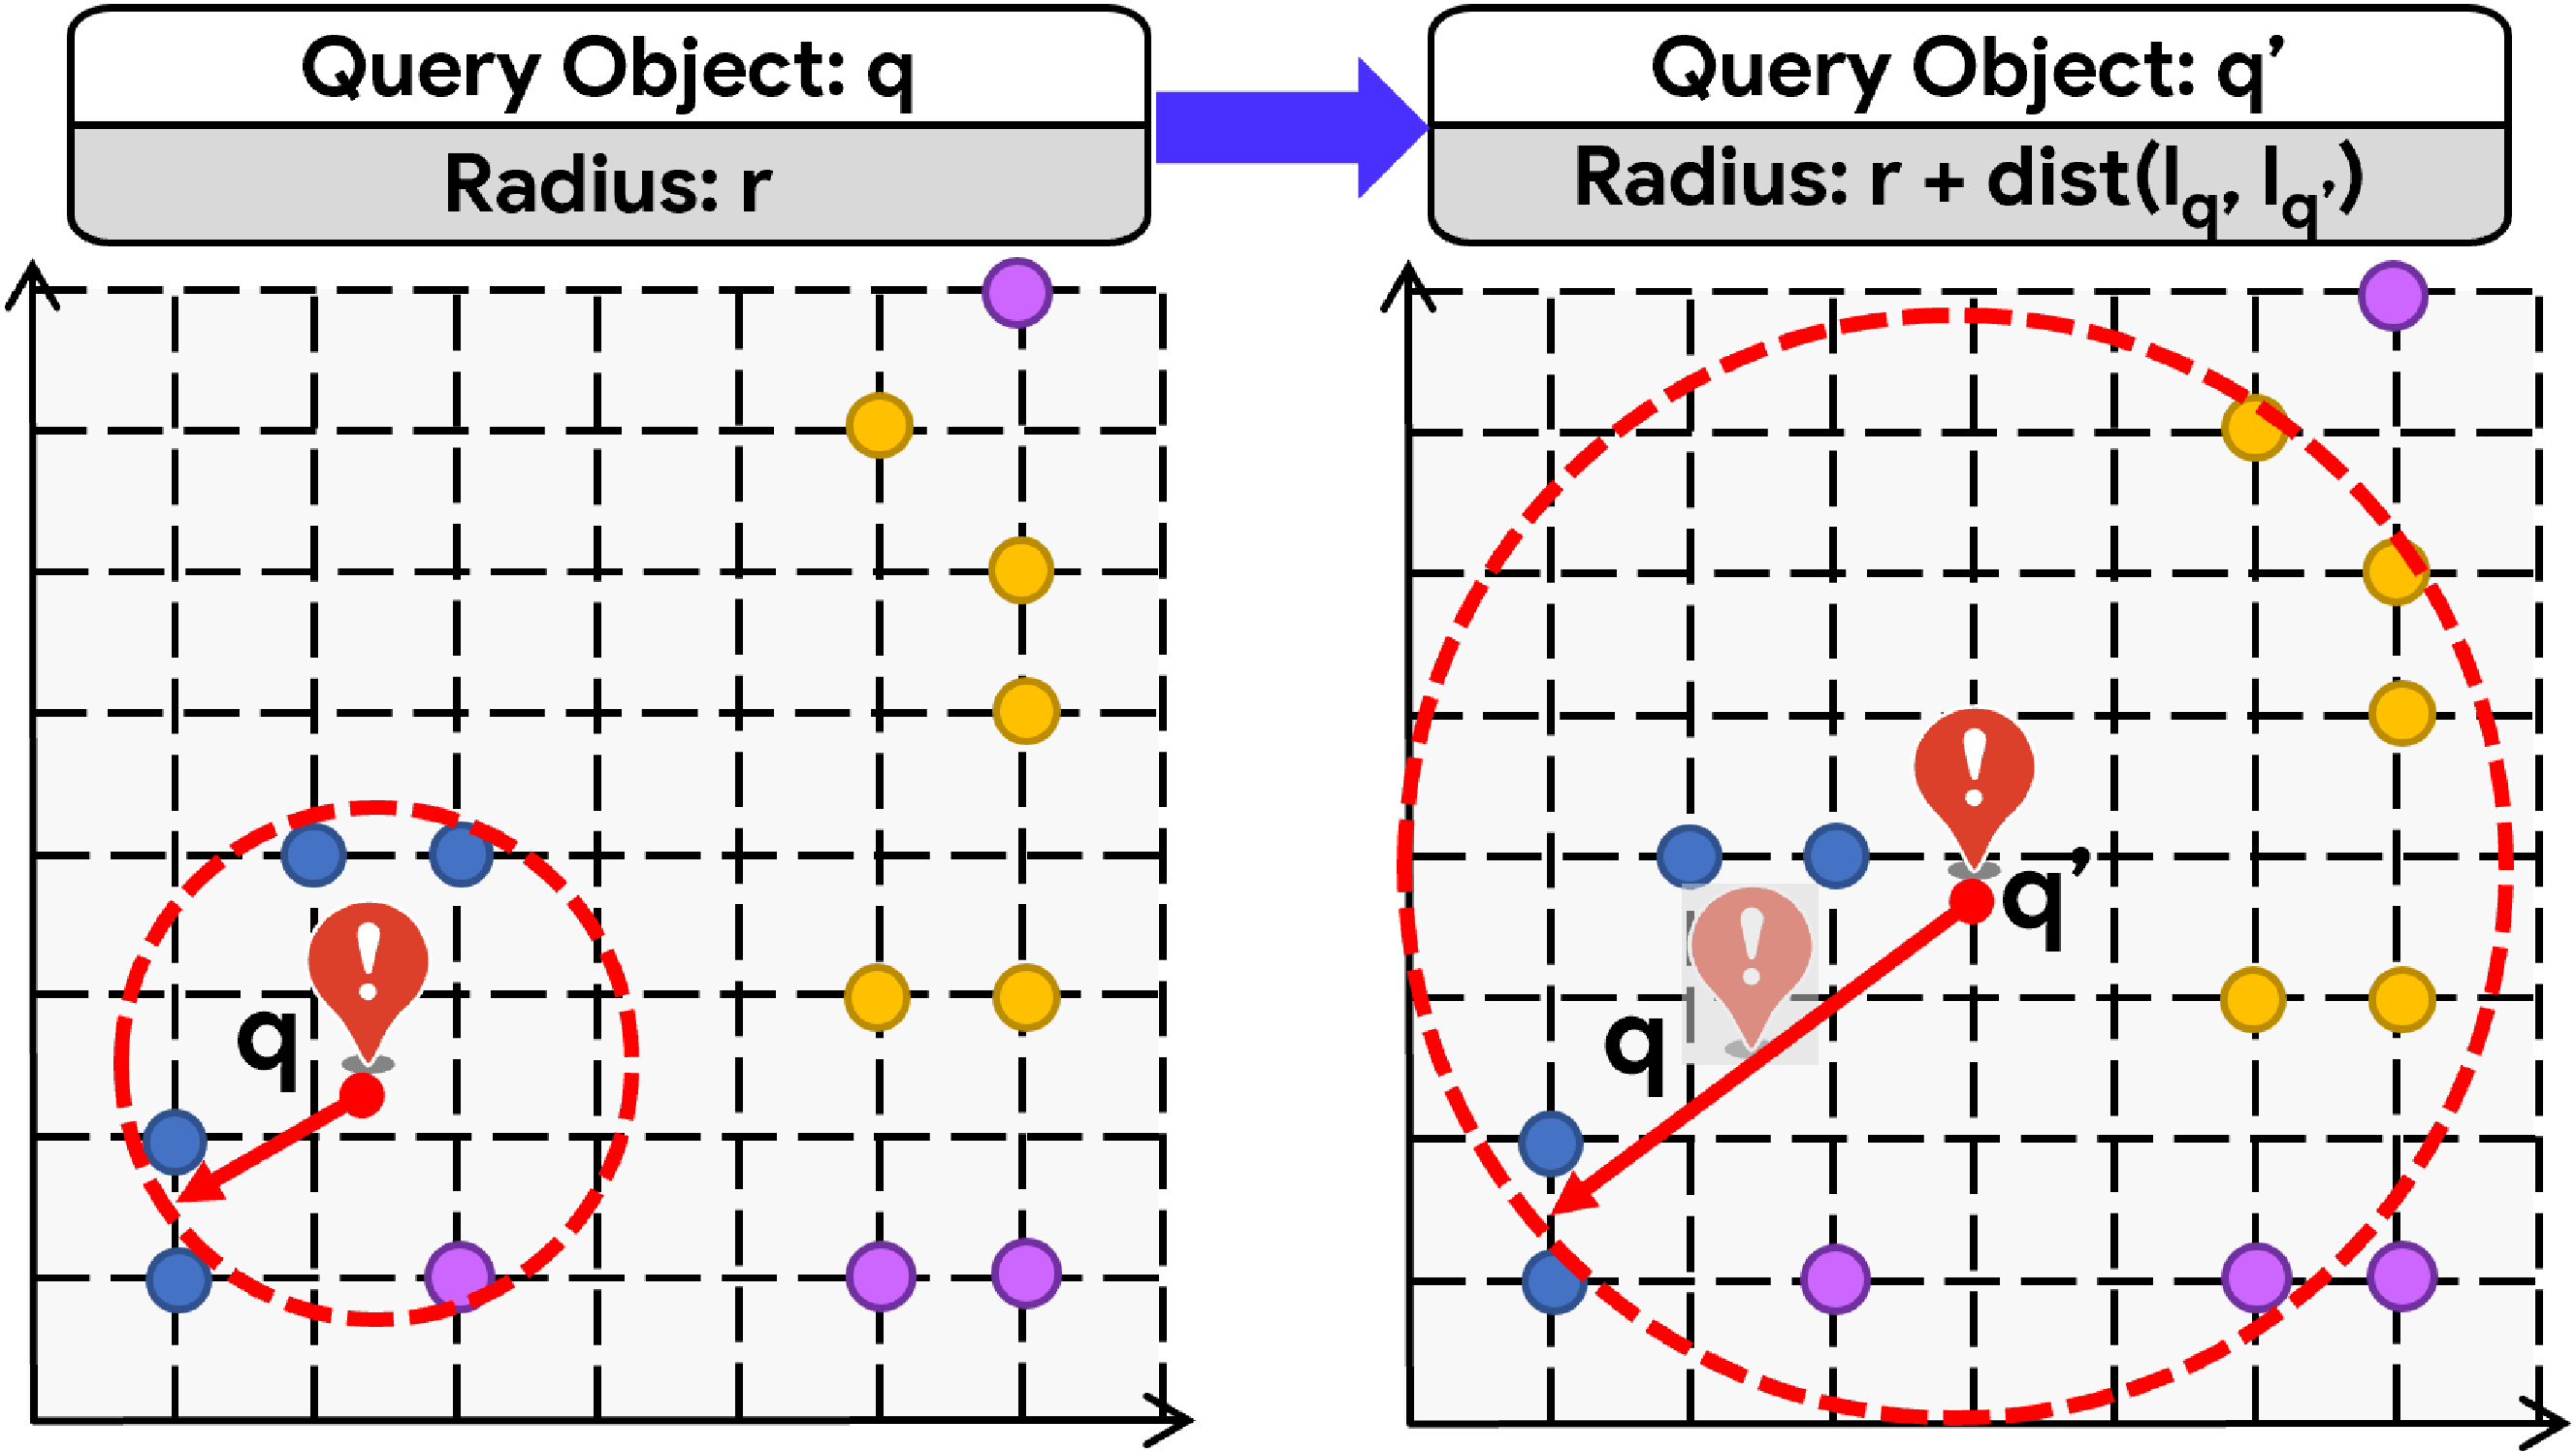
\includegraphics[width=\linewidth]{fed-rq-perturb.pdf}
        \caption{Example for federated range query by \algref{alg:rq}}
		\label{fig:exp-rq-perturb}
   \end{subfigure}
   ~~~
   \begin{subfigure}{0.45\textwidth}
        \centering
        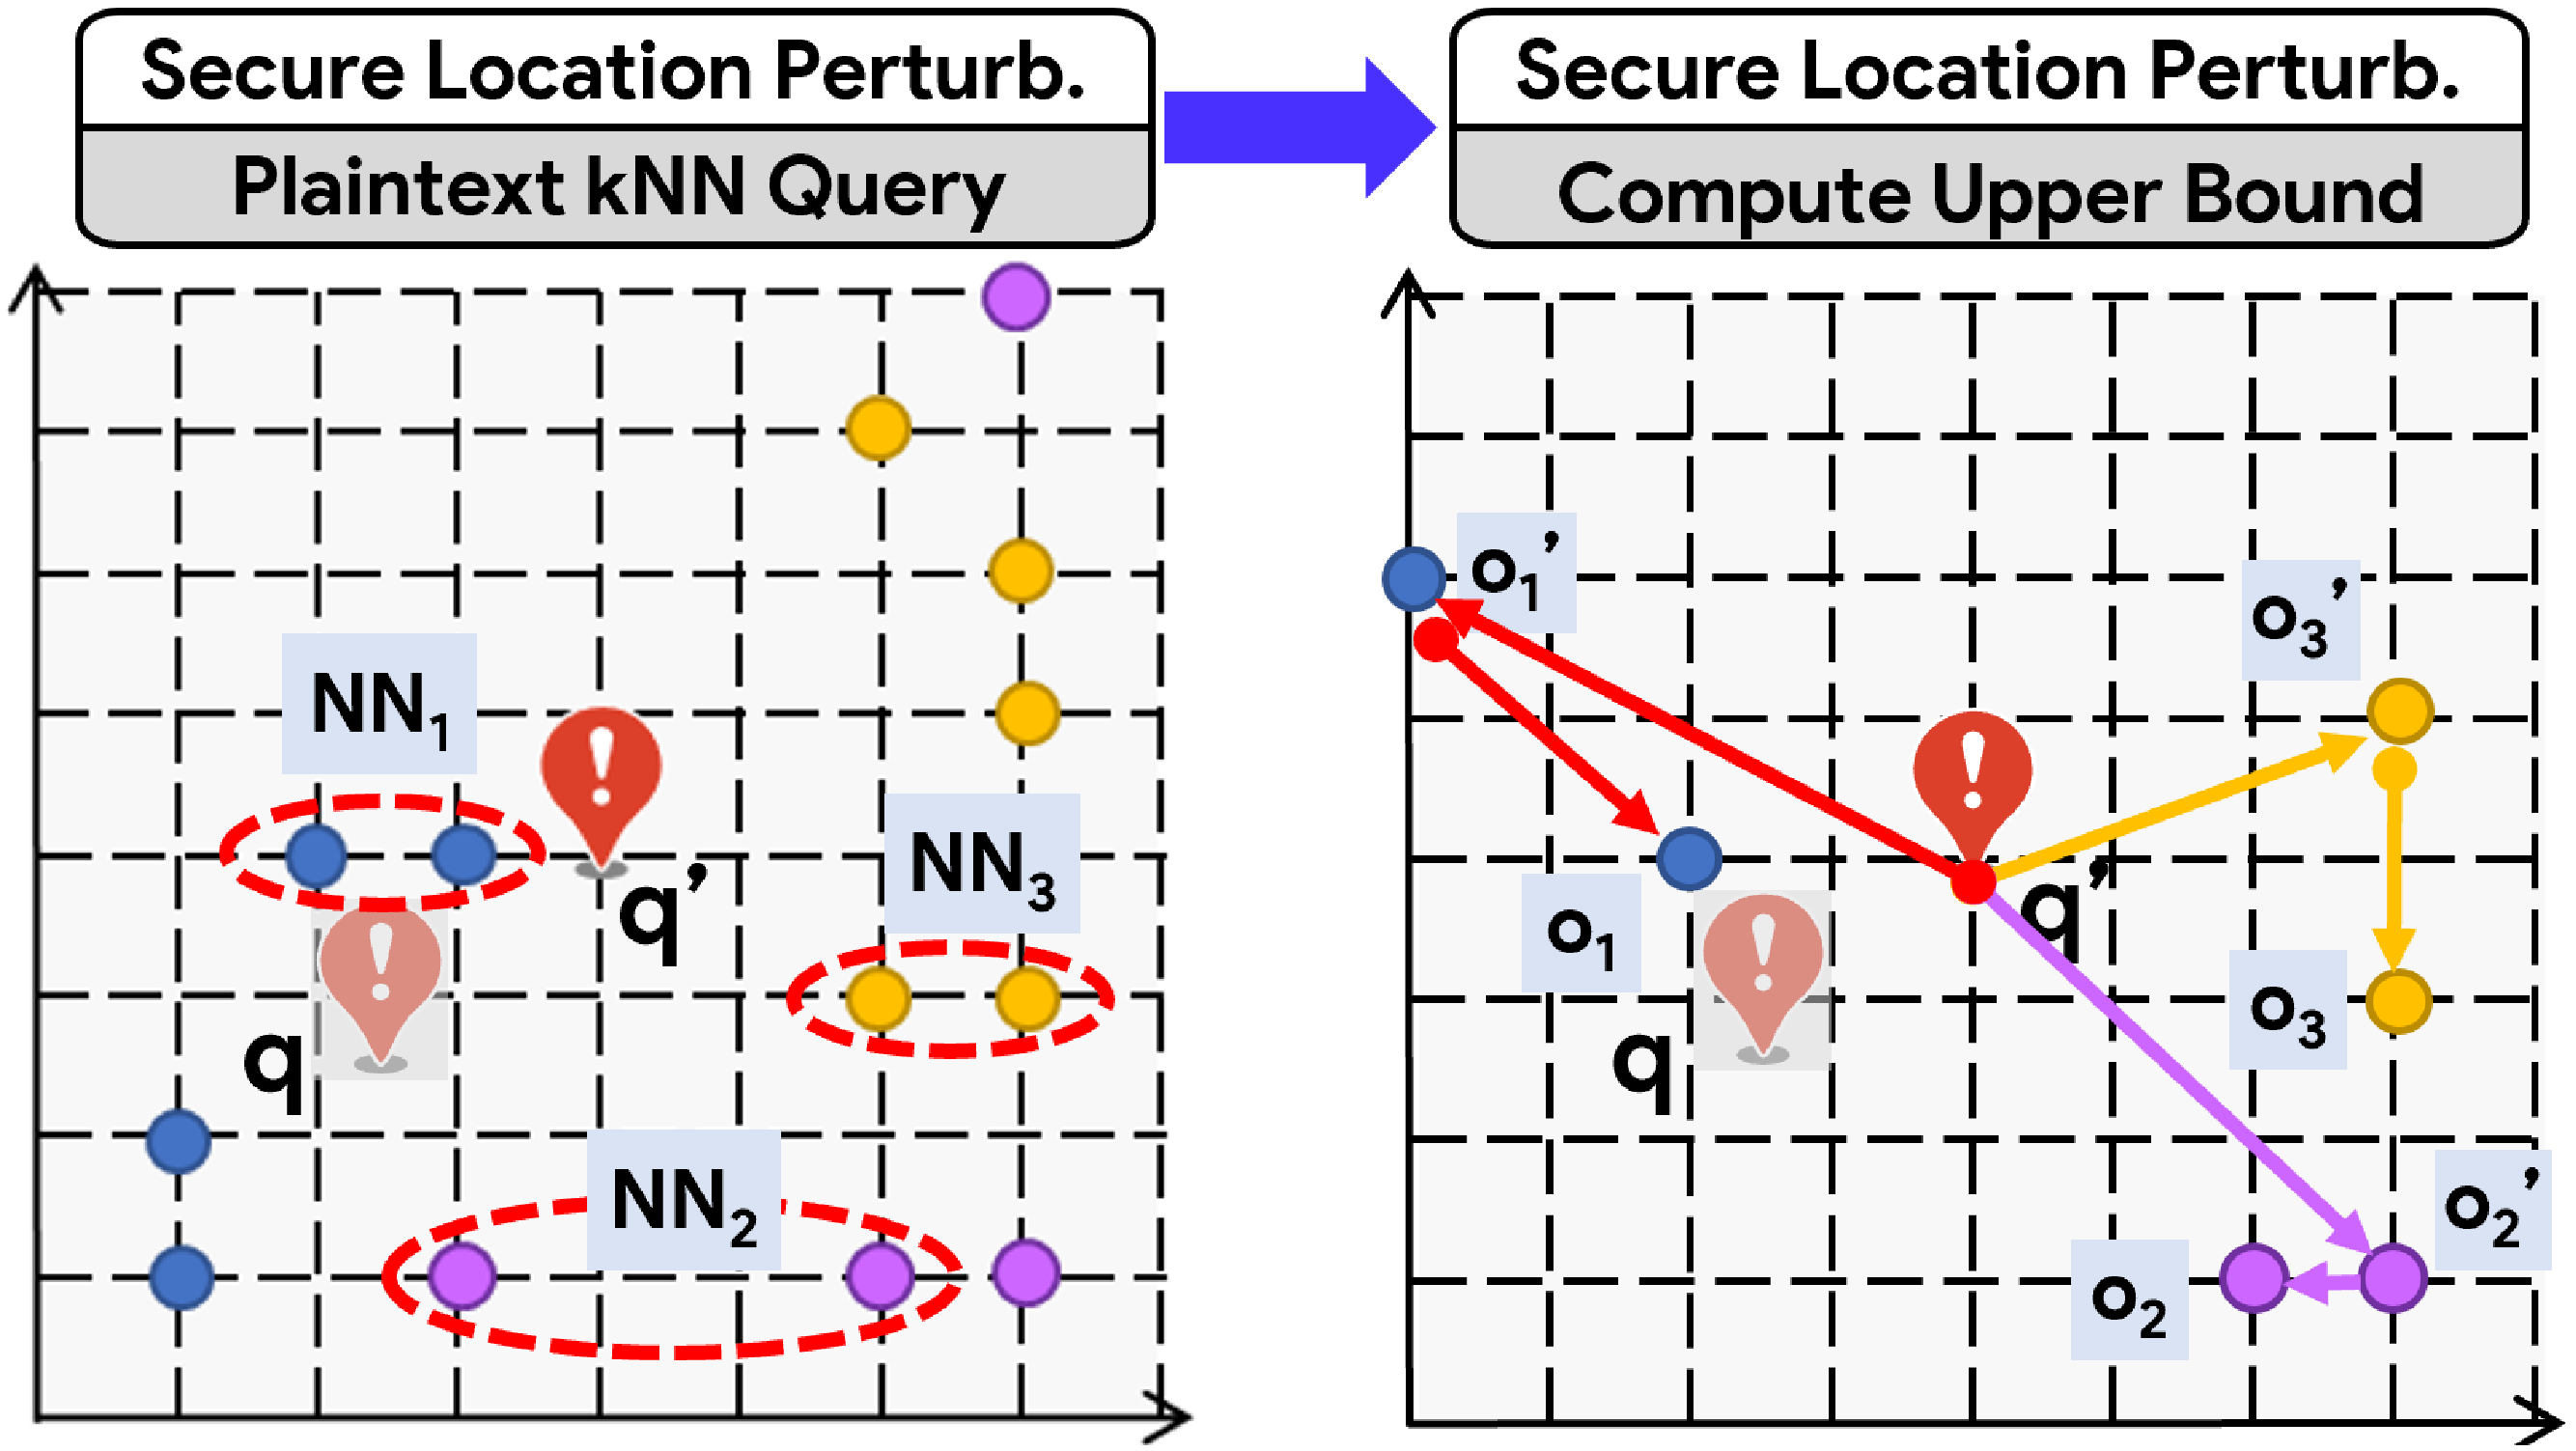
\includegraphics[width=\linewidth]{fed-knn-perturb.pdf}
        \caption{Example for federated kNN query by \algref{alg:knn-UB}}
		\label{fig:exp-knn-perturb}
    \end{subfigure}
    \caption{Examples for decomposing (symmetric) federated range query and kNN query}
    \label{fig:exp-perturb}
\end{figure*}

\begin{example}
    \figref{fig:exp-rq-perturb} presents an illustrative example for \algref{alg:rq}.
    Suppose the query object $q$ is located at $(2.5, 2.5)$ and the radius $r$ of the circular query range is $1.6$.
    By using the \textit{secure location perturbation} operator, $q$ is obfuscated into $q'$ located at $(4, 4)$, so the radius $r'$ is increased to $1.6 + \sqrt{(2.5-4)^2+(2.5-4)^2} = 3.7$ (lines 1-2 of \algref{alg:rq}).
    After executing the \textit{plaintext range query} operator with the expanded query range, we identify 3, 2, and 5 candidates (marked in different colors) in all three silos (line 3).
    Finally, each candidate is further refined by the \textit{secure distance comparison} operator.
\end{example}

\fakeparagraph{Extension to Other Radius-Known Queries}
The decomposition plan for \textit{federated range counting} is almost identical to \algref{alg:rq}. 
The key difference lies in line 7, where federated range counting only needs to aggregate the counts.
When dealing with \textit{federated distance join}, it is initially converted into a series of (symmetric) \textit{federated range queries}. 
Subsequently, each federated range query is decomposed by \algref{alg:rq}.

\subsubsection{Decomposing Radius-Unknown Queries}\label{sec:symmetric-urad}

Similar to the binary search procedure in \algref{alg:knn}, a symmetric \textit{federated kNN query} can be broken down into multiple rounds of (symmetric) radius-known queries.
Besides, \textit{federated kNN join} can still be decomposed into a series of independent federated kNN queries.
Thus, we focus primarily on the necessary modifications for federated kNN queries in the following.

\fakeparagraph{Naive Decomposition Plan}
A naive extension of \algref{alg:knn} can be time-consuming due to the trivial upper bound of the search radius.
If the initial upper bound is set too high, the decomposed radius-known queries will require a large number of secure distance operations, which becomes the major efficiency bottleneck.

\fakeparagraph{Optimized Decomposition Plan}
To overcome the limitation of the naive method, we devise \algref{alg:knn-UB} to compute a tighter upper bound based on the perturbed location. 
Specifically, line 1 perturbs the query object $q$ into $q'$ privately.
In line 2, plaintext kNN query is performed in each silo to identify the $k$ nearest neighbors to $q'$.
However, we cannot send the $k$th nearest distances to the user's client as the upper bound, since it leaks information about locations in the data silos.
Instead, each silo obfuscates the $k$th nearest neighbor $o_i \in NN_i$ into a noised spatial object $o_i'$ (lines 3-4).
In line 5, each silo locally computes its own upper bound $U_i$ and sends it to the user's client.
Finally, the upper bound can be safely set as the minimum value among $\{U_i\}$ (line 6).

\setlength{\textfloatsep}{1ex}
\setlength{\floatsep}{1ex}
\begin{algorithm}[t]
	\caption{\small{Compute tight upper bound for optimizing symmetric federated kNN query}}
    \label{alg:knn-UB}
	\KwIn{federation $F$, query object $q$,  integer $k$}
	\KwOut{the upper bound $U$ for binary-search radius}
    $q' \gets$ secure location perturbation $\geoi(q)$\;
    \ForEach(// perform in parallel){silo $F_i \in F$}{
    $NN_i \gets$ plaintext kNN query $\knn(F_i,q',k)$
    }
    $o_i \gets \arg\max_{o \in NN_i}\{\dist(l_o, l_{q'})\}$\;
    $o_i' \gets$ secure location perturbation $\geoi({o_{i}})$\;
    $U_i \gets \dist(l_{q'}, l_{o_i'}) + \dist(l_{o_i'}, l_{o_i})$\;
    \KwRet{$U \gets \dist(l_q, l_{q'}) + \min\{U_i\ |\ i = 1, \cdots, n\}$}\;
\end{algorithm}
\afterpage{\global\setlength{\textfloatsep}{\oldtextfloatsep}}
\afterpage{\global\setlength{\floatsep}{\oldfloatsep}}

\begin{example}
    \figref{fig:exp-knn-perturb} illustrates \algref{alg:knn-UB}.
    In line 1, the query object $q$ located at $(2.5, 2.5)$ is perturbed into the object $q'$ located at $(4, 4)$.
    Each silo then performs a \textit{plaintext kNN query} with $k=2$ on $q'$.
    The top-2 nearest neighbors in three silos are denoted by $NN_1$-$NN_3$, where $o_i$ is the farthest object to $q'$ within $NN_i$.
    For example, the object $o_1$ at $(2, 4)$ has a distance of 2 to $q'$.
    However, revealing this distance directly may leak spatial information about $o_1$.
    Instead, \algref{alg:knn-UB} leverages a \textit{secure location perturbation} operator to obfuscate $o_1$ to $o_1'$ located at $(0, 6)$.
    Similarly, $o_2$ and $o_3$ are perturbed to $o_2'$ and $o_3'$, respectively.
    Based on the Euclidean distances, we have $U_1 = 7.30$, $U_2 = 5.16$, and $U_3 = 5.24$ (line 5).
    Finally, we pick the minimum from $\{U_i\}$ and derive the tight upper bound $U = 5.16 + 2.12 = 7.28$.
\end{example}

The correctness of \algref{alg:knn-UB} is proved in \lemref{lem:knn-UB}.
\begin{lemma}\label{lem:knn-UB}
    The upper bound $U$ in \algref{alg:knn-UB} is no shorter than the $k$th nearest distance to the query object $q$ in the data federation $F$.
\end{lemma}
\begin{proof}
    Let $d^*$ denote the $k$th nearest distance to $q$, so $d^*$ should satisfy the following inequality:
    \begin{equation}\label{equ:knn-UB-1}
        d^* \le \max\{\dist(l_q, l_{o})\ |\ o \in NN_i\}, \forall i \in [1,n] 
    \end{equation}
    According to the triangle inequality, we have
    \begin{equation}\label{equ:knn-UB-2}
        \dist(l_q, l_{o}) \le \dist(l_q, l_{q'}) + \dist(l_{q'}, l_{o})
    \end{equation}
    Based on \equref{equ:knn-UB-1} and \equref{equ:knn-UB-2}, we can derive that
    \begin{equation*}\label{equ:knn-UB-3}
        d^* \le \dist(l_q, l_{q'}) + \max\{\dist(l_{q'}, l_{o})\ |\ o \in NN_i\}, \forall i \in [1,n] 
    \end{equation*}
    Since $\max\{\dist(l_{q'}, l_{o})\ |\ o \in NN_i\} = \dist(l_{q'}, l_{o_i})$ based on the line 3 of \algref{alg:knn-UB}, we have
    \begin{equation*}\label{equ:knn-UB-4}
        d^* \le \dist(l_q, l_{q'}) + \dist(l_{q'}, l_{o_i}), \forall i \in [1,n] 
    \end{equation*}
    Based on the triangle inequality for $\dist(l_{q'}, l_{o_i})$ and the definition of $U_i$ in line 5 of \algref{alg:knn-UB}, we have
    \begin{align}
        d^* &\le \dist(l_q, l_{q'}) + \big(\dist(l_{q'}, l_{o_i'}) + \dist(l_{o_i'}, l_{o_i}) \big)  \nonumber \\
        & \le \dist(l_q, l_{q'}) + U_i \label{equ:knn-UB-5}
    \end{align}
    According to the inequality in \equref{equ:knn-UB-5} and the definition of $U$ in line 6, we can now prove $d^* \le U$.
\end{proof}

\rev{\fakeparagraph{Remark}
In \algref{alg:knn-UB}, the $k$ nearest neighbors $NN_i$ of the perturbed location $q'$ are used to derive the upper bound.
Notice that $\{NN_i\}$ do not necessarily encompass all the query results of the original location $q$.
By contrast, with \lemref{lem:knn-UB},
the federated range query\slash counting during the binary-search can ensure that
the candidate set includes the exact kNN of $q$.}

\subsection{Discussion}
\label{sec:discussion}
We provide further discussions on the query rewriter.  
% \rev{Due to the page limitation, please refer to the appendixes for the security proof, algorithm details, or evaluation results related to the following discussions.}

\fakeparagraph{Security of Query Rewriter}
We prove the security of our query rewriter based on the composition lemma in \cite{goldreich2009foundations}. 
The idea is to show the decomposition plans for radius-known queries and radius-unknown queries will not reveal any extra information other than the final result due to the usage of secure operators.
We also present a case study that proves it is hard for a semi-honest adversary to attack \sysname.
Please refer to \appref{app:secure} for the detailed security proof and case study of protecting security under specific semi-honest attack.

% \rev{\fakeparagraph{Handling Ties in kNN Query}
% When processing federated kNN queris, we may encounter with the case, 
% where many spatial objects have the distance of $k$th nearest neighbor distance (denoted by $r^*$) to the query object $q$ (\ie ties in kNN queries).
% To handle ties, we need to address \textbf{two technical issues}: (1) how to identify there are ties, and (2) how to retrieve exactly $k$ spatial objects.
% For the \textbf{first question}, line 8 of \algref{alg:knn} (\ie $sign = 0$) can be used to determine whether the current searching radius covers exactly $k$ objects (\ie the counter case, no ties).
% As for the  \textbf{second question}, suppose $[l, u]$ are the final lower bound and upper bound of $r^*$.
% \textit{Firstly}, we use the federated range query with the circular range $\text{circle}(q,l)$ to cache the desired nearest neighbors (within each silo) that are not ties.
% Denote the total number of such objects as $k_l$.
% \textit{Then}, we only need to randomly pick $k-k_l$ objects from the tied ones.
% To achieve this goal, we sequentially request such spatial objects from all data silos,
% nd set a threshold for the limit of spatial objects that are still required.
% \textit{Lastly}, a secure union operator is used to collect the cached partial answers from all data silo.
% }

\rev{\fakeparagraph{Handling Ties in kNN Queries}  
In federated kNN queries, we may encounter ties 
where multiple spatial objects share the same distance (\ie the $k$th nearest distance $r^*$) to the query object $q$. 
Here, we must resolve \textbf{two technical issues}: (1) identifying the presence of ties, and (2) retrieving exactly $k$ nearest neighbors.
  
(1) Line 8 ($sign = 0$) of \algref{alg:knn} indicates the current search radius covers exactly $k$ objects (\ie no ties).
If $sign \neq 0$ during the binary-search, then there are ties.
  
(2) Once ties are identified, we proceed to retrieve exactly $k$ spatial objects. 
Let $[l, u]$ denote the lower and upper bounds of $r^*$. 
First, we use a federated range query with the circular range $\text{circle}(q,l)$ to cache the nearest neighbors that are not part of the ties. 
We denote the number of these objects as $k_l$. 
Next, we select $k - k_l$ objects from the tied ones by sequentially requesting objects from all data silos until we reach the desired count. 
Finally, we use a secure union operator to collect the cached partial answers from all data silos.}

Please refer to \appref{app:knn-tie} for the complete pseudo-code, example illustrations, and experimental evaluation of our solution to handle the case of ties.

\rev{\fakeparagraph{Extension to Rectangular Query Range}
The decomposition plan for radius-known queries can be extended to accommodate rectangular-shaped of query ranges.
For \textit{asymmetric queries}, the extension can be seamlessly implemented by using plaintext range query\slash counting operators for rectangular query ranges,
which are typically supported by spatial database systems.
For \textit{symmetric queries}, where the query object (\ie the rectangle center) is private, 
our extension proceeds as follows.
We first compute the rectangle's circumscribed circle.  
Next, by querying the circumscribed circle with lines 1-4 of \algref{alg:rq},
we identify potential candidates. 
Finally, we securely verify if a candidate $(x, y)$ lies within the rectangle $[(x_L, x_R), (y_L, y_R)]$ using the Yao's garbled circuit (GC) protocol \cite{DBLP:journals/ftsec/EvansKR18} to check the inequalities 
$x \ge x_L$, $x \le x_R$, $y \ge y_L$, and $y \le y_R$. 
The Yao's GC protocol here can be implemented using ObliVM \cite{DBLP:conf/sp/LiuWNHS15}.}

\fakeparagraph{Beyond Mainstream Spatial Queries}
The query rewriter also supports \textit{aggregation queries}, \eg the aggregate attribute on the result of kNN query or range query.
For example, the range aggregate query can be decomposed similarly to a federated range counting.
\rev{Our solution can be also extended to support \textit{approximate spatial queries} by replacing the exact methods for the plaintext operators with approximate ones.
While this is easy to implement, it may be hard to achieve a good balance between efficiency and accuracy.}

\section{Drivers}
\label{sec:drivers}

In \sysname, a driver is deployed on each data silo, consisting of both \textit{plaintext primitives} (\secref{sec:plaintext-primitives}) and \textit{secure primitives} (\secref{sec:secure-primitives}).
Here, plaintext primitives refer to the implementations of plaintext operators that leverage the local spatial database at each silo.
Secure primitives, on the other hand, indicate our secure protocols tailored for the secure operators defined in \secref{sec:cross-silo}.

\rev{Unlike existing systems \cite{vldb17smcql,eurosys19conclave}, 
\sysname aims to support \textbf{heterogeneous} databases through drivers.
In this way, \sysname can \textit{enhance usability} and \textit{avoid costly data migration} compared to these solutions that assume local databases are \textbf{homogeneous}.
To achieve this, the \textit{main difficulties} include
(1) drivers must integrate with the query rewriter to convert plaintext operators into diverse query formats used by data silos,
and (2) drivers must offer default implementations of plaintext operators for local databases that lack support.}

\subsection{Plaintext Primitives}
\label{sec:plaintext-primitives}

Plaintext primitives implement \textit{plaintext range query, range counting, and kNN query}.
They are implemented as an interface on top of the underlying spatial databases for portability and to harness existing range query and range counting implementations.

\fakeparagraph{Primitive Implementation}
The plaintext primitives are implemented by the underlying spatial databases.
\begin{itemize}
    \item 
    For databases that support these plaintext queries, \eg Simba~\cite{sigmod16simba} and PostGIS~\cite{postgis}, we utilize the built-in functions for these queries or generate the corresponding SQL request.
    For example, in PostGIS \cite{postgis}, a plaintext range counting on silo $F_i$ with the center $p$ and radius $r$ of a circular range can be implemented by requesting the SQL below.
	\begin{lstlisting}[mathescape,xleftmargin=-8ex]
        SELECT COUNT(*) FROM $F_i$ 
        WHERE ST_DWithin(p, $F_i$.location, r);
    \end{lstlisting}
    
	\item
	When databases lack native support for any query, the drivers offer a default implementation based on their supported queries and indexes. 
	For example, GeoMesa~\cite{ds15geomesa} does not inherently support range counting, so we extend range counting by calling a range query and subsequently counting the result size.
\end{itemize}

\fakeparagraph{Time Complexity}
In modern spatial databases, plaintext range query, range counting, and kNN query can take $O(\log{m}+|S|)$, $O(\log{m})$, and $O(\log{m})$ time \cite{DBLP:series/synthesis/2011Mamoulis},
where $m$ is the data size and $|S|$ is the output size.

\fakeparagraph{Remark}
In practice, the actual performance of plaintext primitives depends on the native implementation of the local spatial database at each silo.
Thus, when silos utilize heterogeneous spatial databases, the efficiency of federated spatial queries can be limited by the slowest plaintext primitive (see \secref{subsec:exp-hete}). 

\subsection{Secure Primitives}
\label{sec:secure-primitives}

The secure primitives, including secure summation, count comparison, set union, distance comparison, and location perturbation, are independent of local databases.

\fakeparagraph{Primitive Implementation}
Each secure primitive is optimized with a tailored secure protocol as follows.

\textbf{Secure Summation.} 
This primitive is based on \cite{DBLP:journals/dke/EmekciSAA07}.
Initially, each silo $F_i$ holds a private value $v_i$ and all $n$ silos agree on $n$ distinct public parameters $\{u_i\}$.
Each silo $F_i$ then selects a random polynomial of degree $n-1$ in the form $t_i(x)=(\sum_{k=1}^{n-1}a_{ik}x^k) + v_i$,
where $a_{ik}$ is the random coefficient independently generated by silo $F_i$, and $v_i$ denotes the private value (\ie local count) of silo $F_i$.
These variables are kept secret from others by silo $F_i$.
Next, each silo $F_i$ evaluates its polynomial at the public parameters $\{u_1, \cdots, u_n\}$ and sends the resulting value $t_i(u_j)$ to every other silo $F_j$.
Once the silo $F_j$ receives all values $\{t_i(u_j) | i \neq j\}$ from the other silos, we have 
$S(u_j) = \sum_{i=1}^{n}t_i(u_j)=(\sum_{k=1}^{n-1}(u_j)^k\sum_{i=1}^{n}a_{ik}) + \sum_{i=1}^{n}v_i$.
Afterward, this silo sends $S(u_j)$ to the query user.
The user can interpret each $S(u_j)$ as a linear equation $S(u_j)=\sum_{k=1}^{n-1}(u_j)^k z_k + z_n$ in $n$ unknown variables $z_k$,
where $z_k=\sum_{i=1}^n a_{ik}$ (for $k < n$) and $z_n=\sum_{i=1}^n v_i$.
Now, the user can solve the system of linear equations using the received coefficients $\{u_j\}$ and constants $\{S(u_j)\}$ via Gauss elimination, and obtain the unknown variable $z_n$ (\ie the sum of $v_i$).

\textbf{Secure Count Comparison.}
The primitive compares the constant $k$ with the sum of each silo $F_i$'s private range count $v_i$ and prevents the leakage of either $v_i$ or $\sum_{i=1}^nv_i$ to the silo $F_j$ and the query user.
The \textit{main idea} is evaluating $X(\sum_{i=1}^nv_i - k)$ rather than directly computing $\sum_{i=1}^nv_i - k$ to avoid disclosing the actual sum of $v_i$, where $X$ is a positive random number.
Next, we implement this secure primitive by using existing secure multiplication protocol \cite{DBLP:conf/esorics/BogdanovLW08}.
Specifically, this protocol \cite{DBLP:conf/esorics/BogdanovLW08} assumes that two multiplicands, $X$ and $Y$, are partitioned into $n$ shares $x_i$ and $y_i$, where $X=\sum_{i=1}^n{x_i}$ and $Y =\sum_{i=1}^n{y_i}$.
Each silo $F_i$ holds the corresponding shares $x_i$ and $y_i$,
where $x_i$ is randomly generated by this silo and $y_i = v_i - \frac{k}{n}$.
Together, the multiplication $XY$ happens to be $(\sum_{i=1}^nx_i)(\sum_{i=1}^n{v_i} - k)$.
Finally, the comparison result is inferred from the sign of $XY$.

\textbf{Secure Set Union.}
We implement this primitive based on the two-phase union method in \cite{DBLP:conf/socialcom/JurczykX11} with additional optimizations.
In the first phase, each silo appends its results into a global set, along with some fake records.
Then, in the second phase, these fake records are removed from the set. 
To reduce the communication cost, the number of fake records should be as few as possible.
Thus, we use the Laplace mechanism \cite{DBLP:series/synthesis/2016Li} in differential privacy to control the number of fake records.
Moreover, by splitting the global set into batches, parallel executions are enabled for each silo to independently append and remove fake records from each batch, thereby resulting in a shorter latency.

\textbf{Secure Distance Comparison.}
We leverage fully homomorphic encryption (FHE), the BGV scheme \cite{DBLP:journals/csur/AcarAUC18}, to implement this primitive in three key steps.

(1) \textbf{Encrypt User's Data}: the query user encrypts their location $(x_q, y_q)$ and the threshold $r$ using the public key, \ie $E(x_q), E(y_q), E(r)$, where $E(\cdot)$ is the encryption function. The encrypted data and public key are then sent to the data silo.

(2) \textbf{Compute Garbled Distance Difference}: by using FHE, the data silo computes the encrypted difference $E(\Delta)$ between the square of distance $\dist(l_q, l_o)$ and square of threshold $r$ as follows:
\begin{small}
\begin{align*}
    \Delta &= \dist(l_q, l_o)^2 - r^2 = (x_q-x_o)^2 + (y_q-y_o)^2 - r^2 \\
    E(\Delta) &= (E(x_q)-E(x_o))^2 + (E(y_q)-E(y_o))^2 - E(r)^2
\end{align*}
\end{small}
To further obfuscate the value of $E(\Delta)$, the silo applies a random polynomial function $f(\cdot)$ that only has odd powers and positive coefficients in each term,
The obfuscation here prevents the user from inferring the exact distance $\dist(l_q, l_o)$ after decryption, thereby protecting the silo's location privacy.

(3) \textbf{Decrypt}: upon receiving $f(E(\Delta))$ from the silo, the user decrypts it with the secret key and obtains $f(\Delta)$. The final result is derived based on the sign of $f(\Delta)$ without knowing the exact value of $\Delta$.

\textbf{Secure Location Perturbation.}
We implement this primitive based on the BPL mechanism in \cite{DBLP:journals/corr/abs-2312-12012}.
This mechanism obfuscates the original location $(x, y)$ in the polar coordinate system.
The polar angle $\theta$ is uniformly sampled from $[0, 2\pi]$.
The polar radius $r$ is sampled based on the $-1$ branch of the Lambert W function.
If the sampled radius $r$ is too long, it will be truncated into a random value in $[0, R]$,
where $R$ is a safe upper bound of radius based on the privacy parameters $\epsilon,\delta$. 
The resulting perturbed locations are $(x+r\cos{\theta}, y+r\sin{\theta})$.

\fakeparagraph{Complexity Analysis}
The \textit{secure summation} takes $O(n^3)$ time and $O(n^2)$ communication cost.
The \textit{secure count comparison} requires $O(n)$ time and $O(n^2)$ communication cost.
The time complexity and communication cost of \textit{secure set union} are $O(n+|S|)$,
where $|S|$ is the output size.
The \textit{secure distance comparison} (between two parties) takes $O(1)$ time and communication cost,
since the complexity of the BGV scheme \cite{DBLP:journals/csur/AcarAUC18} used for this primitive primarily depends on constant security parameters. 
The time complexity and communication cost of \textit{secure location perturbation} are also $O(1)$ due to the usage of differential privacy mechanism.


\section{Query Interface}
\label{sec:interface}

For easy usability, the query interface of \sysname offers a unified federation view to users (\secref{sec:interface-view}) and supports federated spatial queries in SQL (\secref{sec:interface-SQL}).

\subsection{Unified Federation View}
\label{sec:interface-view}
\sysname's query interface provides a federation view to users, while the detailed information of silos is hidden. 
This not only enables users to send queries without caring about the silo organization, but also protects the data privacy of individual silos.

We implement this unified federation view by extending the schema manager of Calcite~\cite{DBLP:conf/sigmod/BegoliCHML18}, a popular query processing framework.
In Calcite's schema manager, each table is independent and indivisible.
We treat silos as an abstraction layer below the table of schema manager.
This means each table comprises multiple silo objects, and each object records the identity information of its silo.
The silo identities are used when executing secure primitives. 
Specifically, the query rewriter will attach the identity information of all silo-level tables in the table of schema manager when distributing secure operators.
Each silo only executes the corresponding secure primitives if the attached identity information matches the one locally stored.

\subsection{Federated Spatial Queries in SQL}
\label{sec:interface-SQL}
Based on the unified federation view, \sysname query interface supports federated spatial queries in SQL by extending the SQL parser of Calcite with four keywords: {\ttfamily{DWithin}}, {\ttfamily{kNN}},
{\ttfamily{Private\_DWithin}}, and {\ttfamily{Private\_kNN}}.
The first two keywords are used in asymmetric queries, and the last two are used in symmetric queries.

For example, an asymmetric federated range counting on a circular range centered at the point $p$ with radius $r$ can be expressed in SQL as
\begin{lstlisting}[xleftmargin=1.0ex]
  SELECT COUNT(*) FROM F 
  WHERE DWithin(p, F.location, r)
\end{lstlisting}
The {\ttfamily{WHERE} clause checks} whether the distance from $p$ to an object in $F$ is shorter than $r$.
Similarly, an asymmetric federated kNN join on a relation $R$ and federation $F$ can be written in SQL as
\begin{lstlisting}
    SELECT R.id, F.id 
    FROM R JOIN F
    ON kNN(R.location, F.location, k)
\end{lstlisting}
The {\ttfamily{WHERE}} clause indicates whether a spatial object in $F$ belongs to the kNN set of the query point $o\in R$. 

In contrast, when locations in both $R$ and $F$ need protection, a symmetric federated kNN join in SQL is
\begin{lstlisting}
    SELECT R.id, F.id 
    FROM R JOIN F
    ON Private_kNN(R.location, F.location, k)
\end{lstlisting}
% A symmetric federated range query in SQL is
% \begin{lstlisting}[xleftmargin=1.0ex]
%   SELECT COUNT(*) FROM F 
%   WHERE Private_DWithin(p, F.location, r)
% \end{lstlisting}
Other federated spatial queries can be written as SQL similarly with these four keywords.

\section{Evaluation}
\label{sec:evaluations}

In this section, we first introduce the experimental setup (\secref{sec:experiment-setup}), and then present the overall performances of asymmetric queries (\secref{subsec:exp-cmp}) and symmetric queries (\secref{subsec:exp-symmetric}), scalability  tests (\secref{subsec:exp-scalability}), and results with heterogeneous spatial databases across silos (\secref{subsec:exp-hete}).

\subsection{Experimental Setup}
\label{sec:experiment-setup}

\fakeparagraph{Datasets}
Experiments are conducted on two datasets, with each object having a location and unique ID.

\begin{itemize}
    \item \textbf{Multi-company Spatial Data in Beijing (BJ).}
    \rev{This dataset\footnote{\rev{https://share.weiyun.com/z4QfVhVv}}} was collected by 10 companies in Beijing, in June 2019, which has $1,029,081$ spatial objects in total.
    The locations of these objects fall into an area from $39.5^{\circ}$N $\sim42.0^{\circ}$N and $115.5^{\circ}$E $\sim117.2^{\circ}$E.
    We use the dataset to simulate a real-world federation, where each company can be naturally regarded as a silo.
    During the evaluation, we vary the silo number $n$ and queries without altering the spatial object distributions across silos.

    \item \textbf{OpenStreetMap (OSM).}
    This is a popular open dataset to evaluate spatial queries.
    We mainly use this dataset in the scalability test, where we sample $10^4$-$10^9$ spatial objects from the Asia dataset in the OpenStreetMap \cite{osm}.
    Specifically, to simulate the spatial overlaps as in the BJ dataset, we assign a random silo ID for each point in the dataset and make each silo have the same number of data points.
\end{itemize}

Please refer to \appref{app:exp-geo} for experiments on geographically partitioned dataset.

\fakeparagraph{General-Purpose Baselines}
As a data federation system, the evaluation first aims to compare \sysname with existing general-purpose data federation systems: the GIS extensions of SMCQL \cite{vldb17smcql} and Conclave \cite{eurosys19conclave}.

\begin{itemize}
    \item \textbf{\smcql.} 
    \rev{It adopts the principles of SMCQL \cite{vldb17smcql}, a garbled circuit (GC) based solution for relational data, to support spatial queries.
    We implement it with ObliVM~\cite{DBLP:conf/sp/LiuWNHS15}, 
    which is used in SMCQL for GC protocols across two silos (only) \cite{eurosys19conclave,DBLP:conf/sigmod/Wang021}.
    Thus, it is only evaluated over two data silos.}
    % \smcqlext is a variant of \smcql without assuming an honest broker, and uses our secure set union operator to assemble the partial results from all silos.
    
    \item \textbf{\conclave.} 
    It adopts the principles of Conclave \cite{eurosys19conclave}, the secret sharing (SS) based solution for relational data, to support spatial queries.
    It is implemented with a different SS based library, MP-SPDZ~\cite{DBLP:conf/ccs/Keller20}, rather than Sharemind \cite{DBLP:conf/esorics/BogdanovLW08} in the original Conclave,
    since Sharemind is devised for only three silos \cite{DBLP:journals/ftsec/EvansKR18} and it is a commercial library.
    In contrast, MP-SPDZ is a popular open-source library that supports more than three silos based on SS.
    %\conclaveext is a variant of \conclave without assuming an honest broker, and uses our secure set union to assemble results.

    \item \textbf{\smcqlext \& \conclaveext} are their variants without assuming an honest broker, and uses our secure set union to assemble results.
\end{itemize}


These secure baselines implement federated spatial queries by exploiting similar queries for relational data in SMCQL or Conclave.
Our extensions follow the strategy of having plaintext spatial queries within each silo's database and securely computing the final results.
Specifically, for \textit{federated range query}, these baselines execute plaintext range query in each silo and collect the partial results by either the honest broker or our secure set union.
For \textit{federated range counting}, they execute plaintext range counting and use secure summation to compute the final result.
For \textit{federated kNN query}, we regard it as a top-k query with a user-defined function (UDF).
For example, each silo runs plaintext kNN query to compute $k$ candidate neighbors along with their distances to the query object. Then, all $n$ silos securely find the $k$ nearest neighbors among $nk$ candidates.
For \textit{federated distance join/kNN join}, we refer to their query plans for join queries and regard a federated distance/kNN join as multiple federated range/kNN queries.

\fakeparagraph{Specialized Baselines}
Beyond these general-purpose data federation systems,
the evaluation also compares \sysname with the following specialized baselines.
\begin{itemize}
    \item \textbf{Additional Baselines for Asymmetric Queries}.
    The plaintext baseline \public directly collects local results from each silo without any secure operation, and serves as the upper bound of query efficiency.

    \item \textbf{Additional Baselines for Symmetric Queries}.
    We consider two more baselines for symmetric queries: \EDBT \cite{DBLP:conf/edbt/KesarwaniKNPSMM18} and \ICDE \cite{DBLP:conf/icde/SahinAAAP18}.
    \EDBT \cite{DBLP:conf/edbt/KesarwaniKNPSMM18} is an industrial solution that utilizes Leveled Fully Homomorphic Encryption (LFHE) and two mutually untrusted servers to securely answer (exact) kNN queries over multiple data silos.
    This solution can be easily extended to support secure range query and counting over a spatial data federation.
    By contrast, \ICDE \cite{DBLP:conf/icde/SahinAAAP18} leverages a differentially private index (\eg grid index for spatial data) and AES encryption \cite{goldreich2009foundations} to approximately answer range queries with small errors.
    However, this method assumes that the user has access to data objects outside the query answer, potentially violating the data privacy requirement.
    Nevertheless, we select \ICDE \cite{DBLP:conf/icde/SahinAAAP18} as a baseline for comparison, since it also utilizes differential privacy for filtering before verifying each candidate through encryption. 
\end{itemize}

\fakeparagraph{Metrics}
We assess the query efficiency by two metrics:

(1) \textbf{Running time} is the time cost from receiving the query to returning the query answer to the user.

(2) \textbf{Communication cost} is the total network communication among the user and all data silos.

%\rev{For each query type, we generate 50 queries, repeat 10 times for each query, and report the average result.}

\fakeparagraph{Implementation}
We use PostgreSQL 10.15 with PostGIS extension as the default spatial database for all silos.
To show the support of heterogeneous spatial data systems by \sysname, we also use MySQL 5.7~\cite{mysql}, SpatiaLite~\cite{spatialite}, GeoMesa 3.0.0~\cite{ds15geomesa}, Simba 1.0~\cite{sigmod16simba}, and SpatialHadoop 2.4.3~\cite{icde15spatialhadoop} as different silos, as will be explained in \secref{subsec:exp-hete}.
They all use spatial indexes (R-Tree in PostGIS, Simba, SpatialHadoop, and MySQL, and R*-Tree in SpatiaLite, and Z-Curve in GeoMesa) to speed up plaintext primitives by up to $2042\times$ (see \appref{appendix:spatial-index}).
Among the compared solutions, \EDBT and \ICDE are implemented in C++, while the others are implemented in Java.
The reason for using C++ for \EDBT and \ICDE is due to the lack of robust and open-source libraries in Java for the encryption methods (\eg CKKS \cite{DBLP:journals/csur/AcarAUC18}) they utilize.
% If the query processing methods in \sysname are implemented in C++, we will further enhance the efficiency.
% For instance, when answering a symmetric federated range queries with the default parameters, the running time can be reduced by  at least $6.9\times$.

\subsection{Experiments on Asymmetric Queries}
\label{subsec:exp-cmp}

\fakeparagraph{Parameter Setting}
In this experiment, we compare the efficiency of different methods for all five federated spatial queries on the real dataset BJ.
All the query points are randomly sampled from the dataset.
We vary the number of silos from $2$ to $10$, and also test the impact of query-specific parameters.
We set $k$ to $16$ for federated kNN query and kNN join, and the default query area of federated range query, range counting and distance join as $0.001\%$, and vary them from $4$ to $64$ and $0.00001\%$ to $0.1\%$ respectively.
The range of these query-specific parameters is aligned with previous study~\cite{sigmod16simba}.
When evaluating the query-specific parameters, we use $6$ silos by default.

\fakeparagraph{Environment} 
We run this experiment on a cluster of $11$ machines.
Each machine has 32 Intel(R) Xeon(R) Gold 5118 2.30GHz processors and 64GB memory with Ubuntu 18.04 LTS. 
The network bandwidth between machines is up to 10 GB/s.
Among the $11$ machines, one is as the user and the honest broker for \smcql and \conclave, and the other 10 are data silos.

% In the following, we present the experimental results and analysis of the federated kNN query, kNN join, range counting, range query, and distance join in \secref{sec:exp-asym-knn} to \secref{sec:exp-asym-rqj}, respectively.
% Finally, the key findings are summarized in \secref{sec:exp-asym-summary}.

\begin{figure}[t]
    \centering
    \begin{subfigure}{0.30\textwidth}
        \centering
        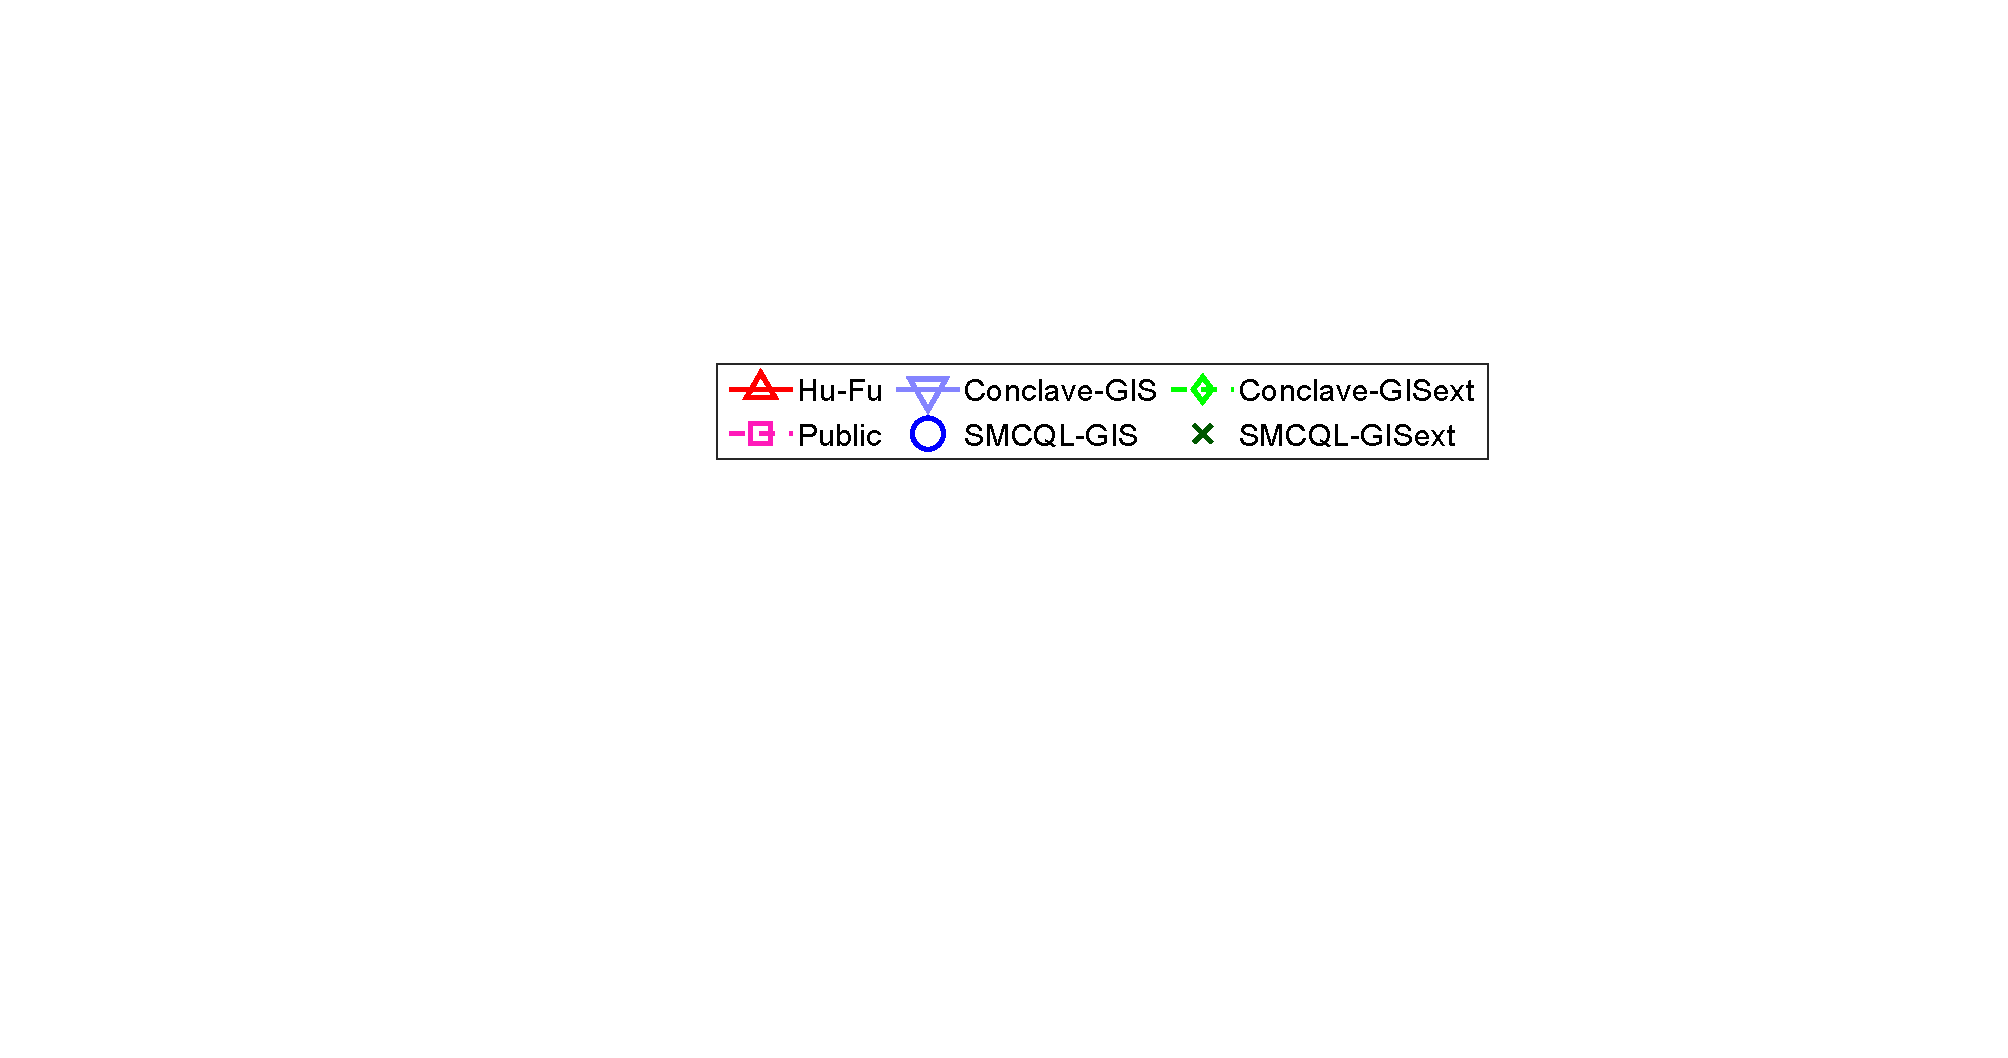
\includegraphics[width=\textwidth]{legend.pdf}
    \end{subfigure}
    \begin{subfigure}{0.48\textwidth}
        \centering
        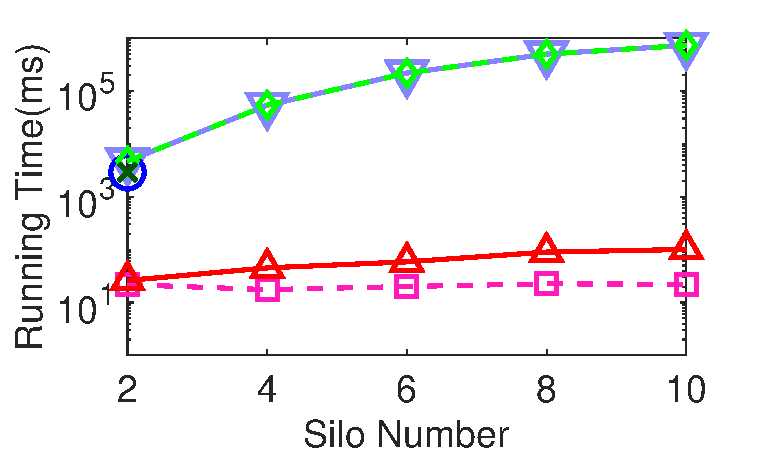
\includegraphics[width=0.48\linewidth]{knn_silo_time.pdf}
        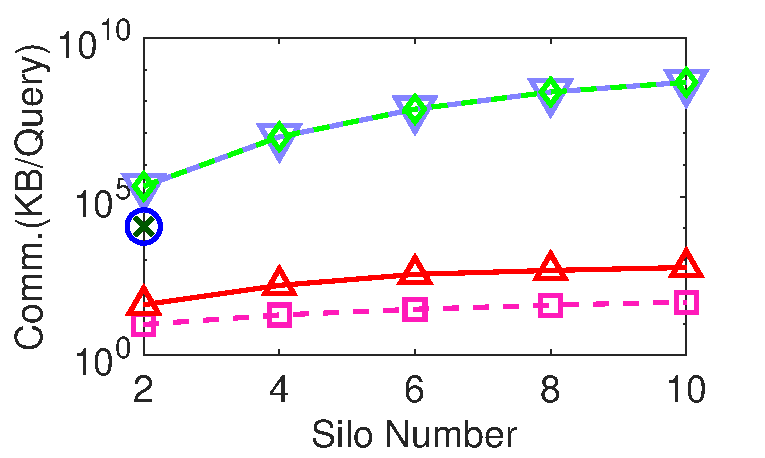
\includegraphics[width=0.48\linewidth]{knn_silo_cost.pdf}
        \caption{Runtime and communication cost of varying silo number}
        \label{fig:knn-eff-silo}
    \end{subfigure}
    \begin{subfigure}{0.48\textwidth}
        \centering
        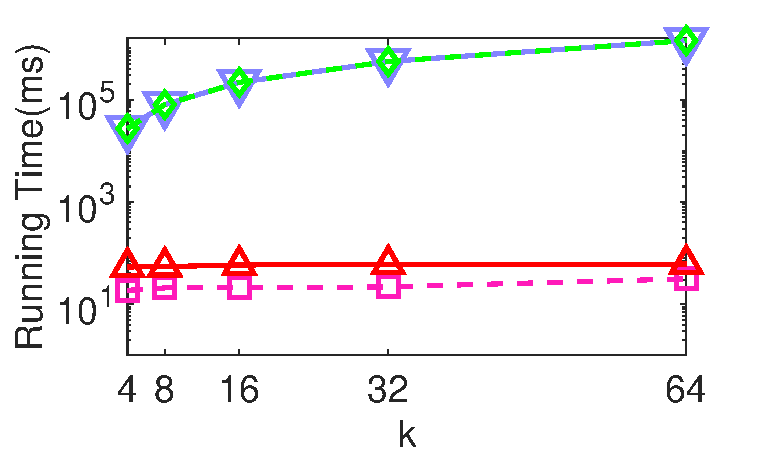
\includegraphics[width=0.48\linewidth]{knn_k_time.pdf}
        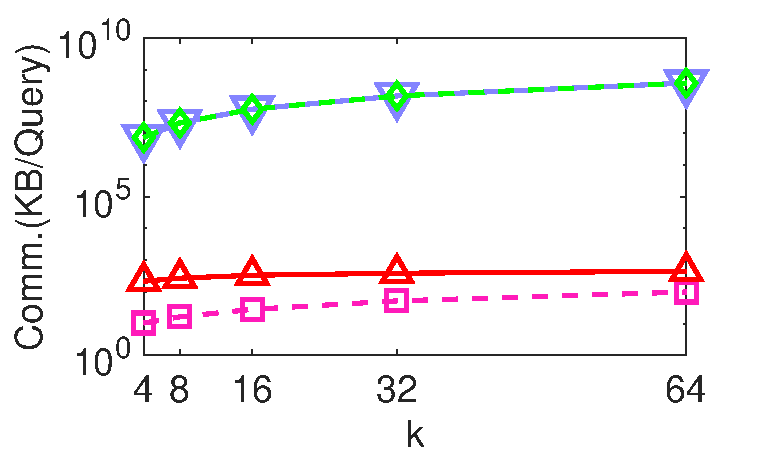
\includegraphics[width=0.48\linewidth]{knn_k_cost.pdf}
        \caption{Runtime and communication cost of varying $k$}
        \label{fig:knn-eff-k}
    \end{subfigure}
    \caption{Performance of federated kNN query.}
    \label{fig:knn-eff}
\end{figure}

% \begin{table}[t]
% \caption{Ablation of DP optimization in federated kNN.}
% \label{tab:dp-opt}
% \begin{small}
% \resizebox{0.48\textwidth}{!}{
% \begin{tabular}{ccccccc}
% \toprule
% \multicolumn{2}{c}{Silo number}  & 2        & 4        & 6        & 8        & 10       \\ \midrule
%        & w/ DP  & 26.1 & 45.1 & 58.6 & 89.6 & 100.5 \\ \cmidrule(l){2-7}
% \multirow{-2}{*}{\begin{tabular}[c]{@{}c@{}}Time\\(ms)\end{tabular}}  & w/o DP & 26.9 & 50.3 & 72.9 & 107.0 & 116.9 \\ \midrule
%    & w/ DP & 39.4    & 160.8   & 357.7   & 475.1   & 588.3   \\ \cmidrule(l){2-7}
% \multirow{-2}{*}{\begin{tabular}[c]{@{}c@{}}Comm.\\(KB)\end{tabular}} & w/o DP & 58.5 & 234.8   & 493.0   & 784.0   & 1125.2   \\ 
% \bottomrule
% \end{tabular}}
% \end{small}
% \end{table}

\begin{table}[t]  
    \caption{Improvement with DP in federated kNN.}  
    \label{tab:dp-opt-percent} 
    \begin{small} 
    \resizebox{0.48\textwidth}{!}{  
    \begin{tabular}{ccccccc}  
    \toprule  
    \multicolumn{2}{c}{Silo number} & 2 & 4 & 6 & 8 & 10 \\ \midrule
    Running time &  &   
    2.9\% & 10.3\% & 19.6\% & 16.2\% & 14.0\% \\ \midrule
    Communication &  &   
    32.6\% & 31.5\% & 27.4\% & 39.4\% & 47.7\% \\ 
    \bottomrule  
    \end{tabular}
    }  
    \end{small}
\end{table}

\subsubsection{Performance of Federated kNN Query}
\label{sec:exp-asym-knn}

\figref{fig:knn-eff-silo} shows the runtime and communication cost of (asymmetric) federated kNN query.
\sysname is $109.6\times$ to $7,198.8\times$ faster than \smcql and \conclave, and has $2$ to $5$ orders of magnitude lower communication cost.
When the number of silos increases from $2$ to $10$, the runtime and communication cost of \sysname only increase by up to $2.9\times$ and $13.9\times$, while those of \conclave drastically increase by up to $153.3\times$ and $1,884.3\times$.
Both metrics of \sysname increase since the secure comparison and set union used in this query grow linearly with the silo number.
Compare with \conclave and \smcql, the runtime and communication cost of \conclaveext and \smcqlext marginally increase (less than 20 ms and 200 KB respectively), which shows that our secure set union can efficiently assemble query results without an honest broker.

We also vary $k$ from $4$ to $64$ and plot the running time and communication cost in \figref{fig:knn-eff-k}.
As $k$ increases from $4$ to $64$, the running time and communication cost of \sysname only increase by $0.1\times$ and $1.1\times$, while those of \conclave increase by $51.3\times$ and $50.7\times$.
The impact of $k$ is less obvious than the silo number on \sysname, because only the secure set union is linearly dependent on $k$.
Again, the efficiency of \conclaveext is similar to that of \conclave.
The drastic increase in running time and communication cost of \conclave and \conclaveext is expected because it involves many secure primitives that are time-consuming.

% Recall that we apply differential privacy (DP) to accelerate kNN queries (see \secref{sec:asymmetric-urad}). 
To show the improvement of DP optimization in kNN queries, 
we list the percentage of running time and communication cost reduced by DP in \tabref{tab:dp-opt-percent}. 
With DP, the running time is reduced by up to $19.6\%$, and the communication cost by up to $47.7\%$.
Compared with the improvement, the overhead of injecting the DP noise is very marginal,
which takes 2 $\mu s$ time cost and less than 1 KB communication cost when processing one federated kNN query. Such a notable improvement is because the complexity of DP noise injection is $O(1)$ and the summation only requires for transmission of $n$ integers, 
while a secure comparison has $O(n)$ time complexity and $O(n^2)$ communication cost.

\begin{figure}[t]
    \centering
    \begin{subfigure}{0.30\textwidth}
        \centering
        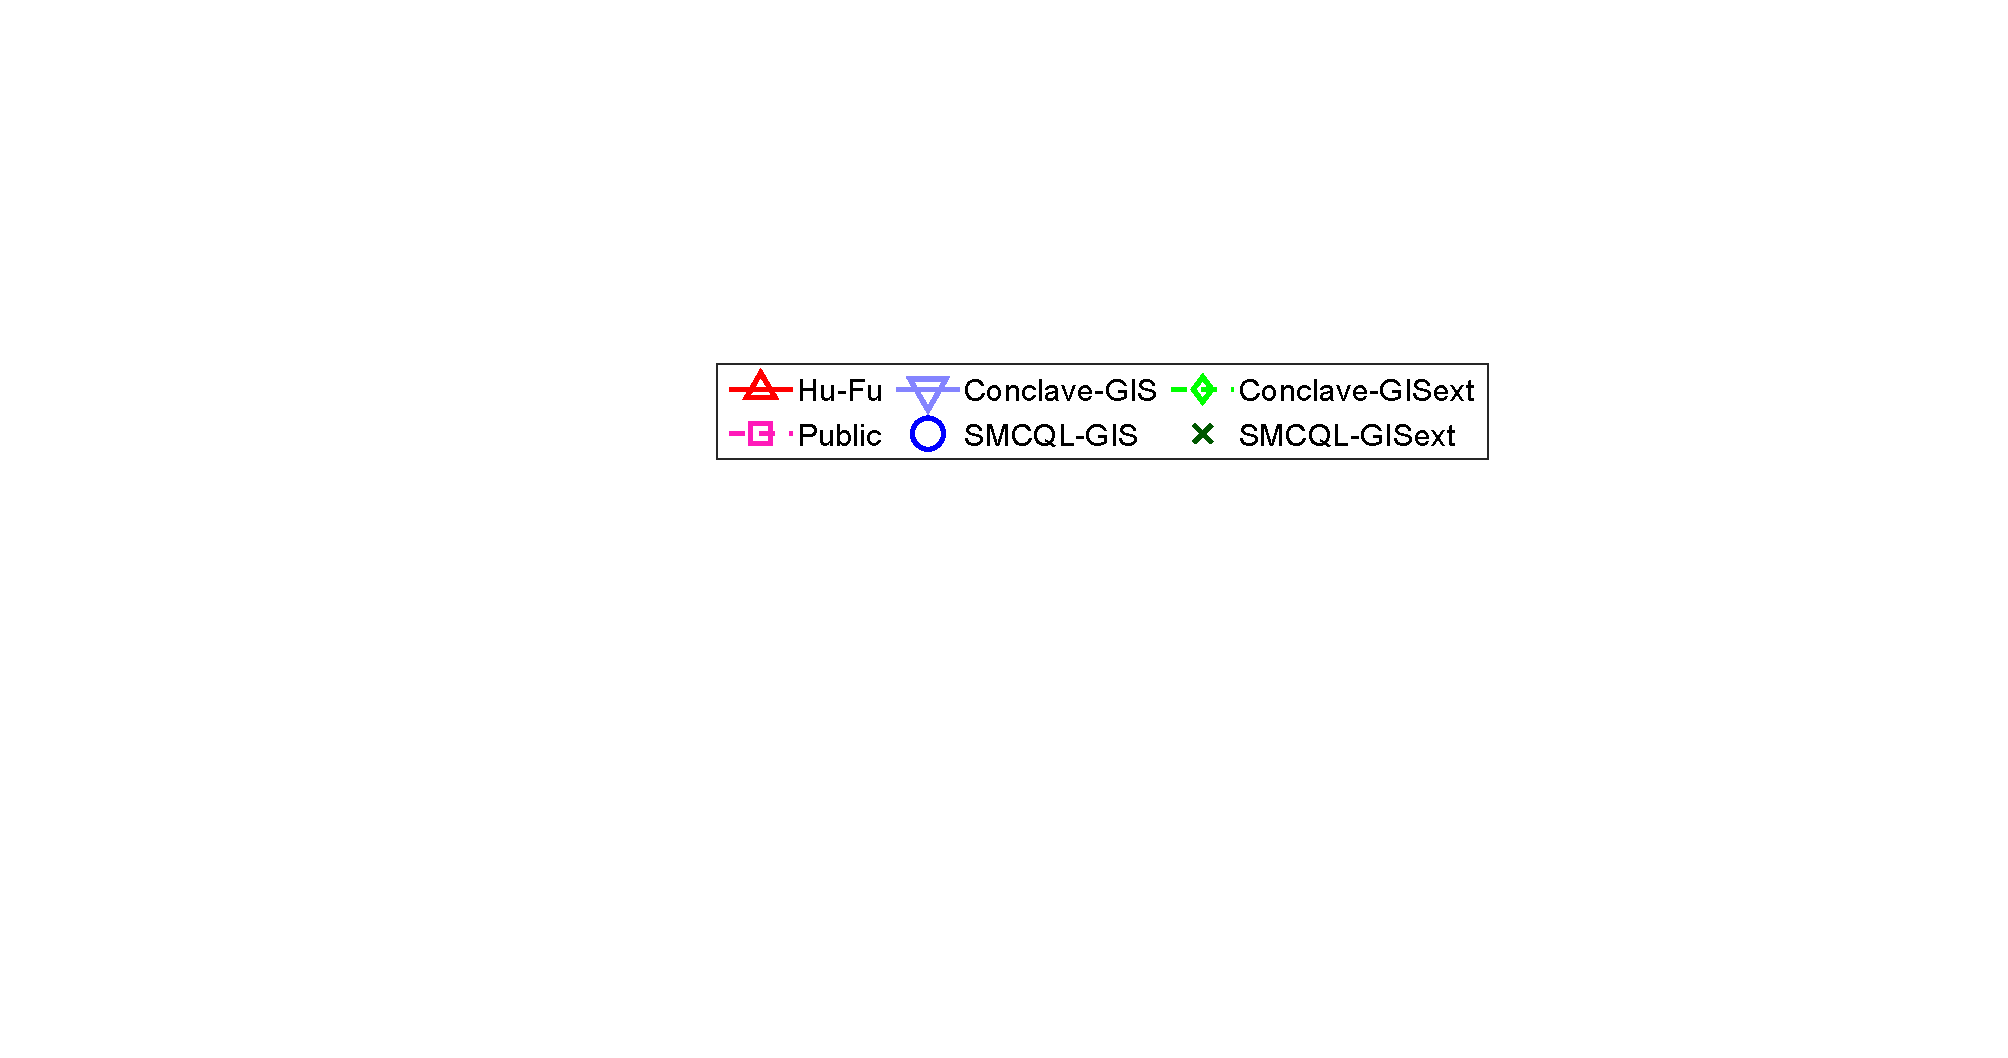
\includegraphics[width=\textwidth]{legend.pdf}
    \end{subfigure}
    \begin{subfigure}{0.48\textwidth}
        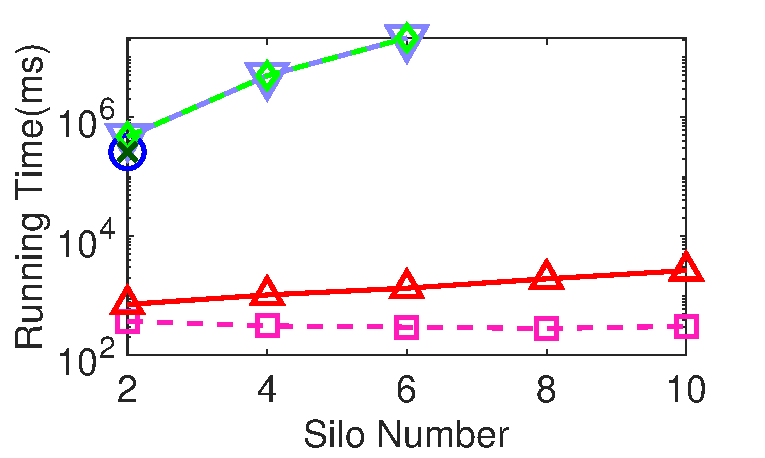
\includegraphics[width=0.48\linewidth]{knnjoin_silo_time.pdf}
        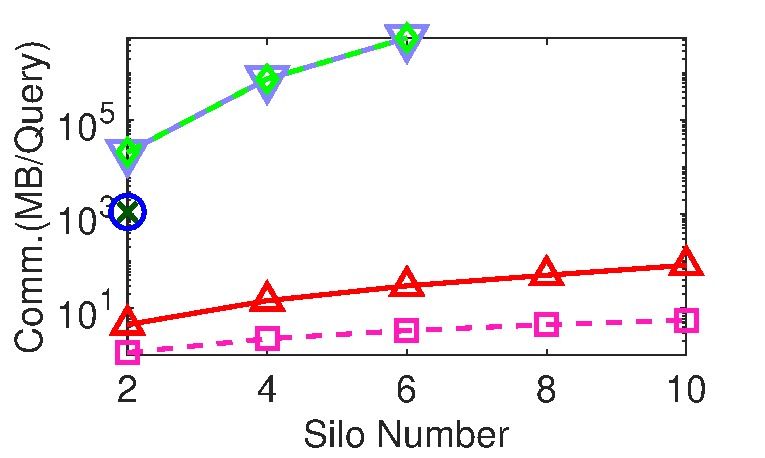
\includegraphics[width=0.48\linewidth]{knnjoin_silo_cost.pdf}
        \caption{Runtime and communication cost of varying silo number}
        \label{fig:knn-join-eff-silo}
    \end{subfigure}

    \begin{subfigure}{0.48\textwidth}
        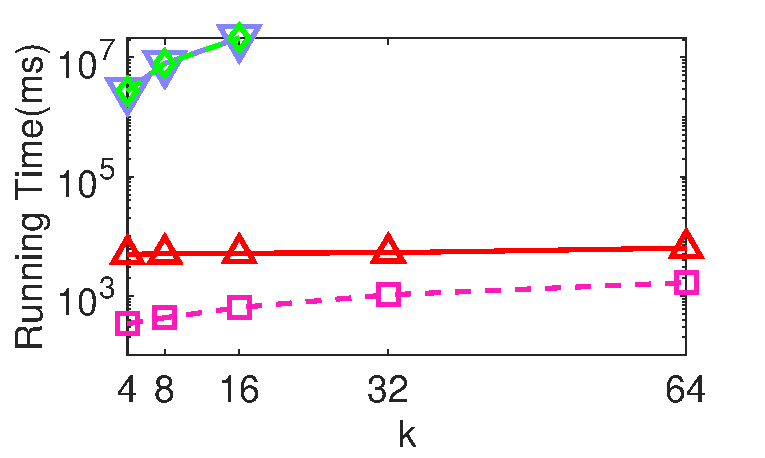
\includegraphics[width=0.48\linewidth]{knnjoin_k_time.pdf}
        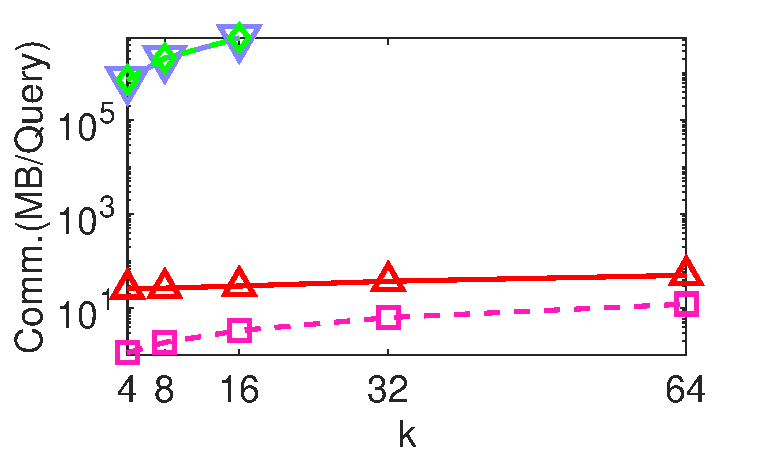
\includegraphics[width=0.48\linewidth]{knnjoin_k_cost.pdf}
        \caption{Runtime and communication cost of varying $k$}
        \label{fig:knn-join-eff-k}
    \end{subfigure}
    \caption{Performance of federated kNN join.}
    \label{fig:knn-join-eff}
\end{figure}

\subsubsection{Performance of Federated kNN Join}
\label{sec:exp-asym-knnj}

\figref{fig:knn-join-eff-silo} shows the results of (asymmetric) federated kNN join.
Results of \conclave and \conclaveext with $8$-10 silos are omitted since they incur over $6$ hours for a single query. 
\sysname is the most efficient, which is up to $360.2 \times$ and $15,814.2 \times$ faster than \smcql and \conclave with $247.8 \times$ and $185,151.0 \times$ lower communication cost.
The time and communication cost of \smcqlext and \conclaveext slightly increase over \smcql and \conclave.

\figref{fig:knn-join-eff-k} illustrates the impact of $k$.
As $k$ increases above 32, \conclave and \conclaveext require longer than 6 hours to process a federated kNN query.
Thus, we can only provide their partial results (when $k \le 16$).
In contrast, \sysname demonstrates superior advantages in the efficiency, achieving at least 553$\times$ faster and 27,404$\times$ lower communication cost compared to \conclave.
As $k$ increases from $4$ to $64$, the running time and communication cost of \sysname rise by $28\%$ and $48\%$ respectively.
The experimental trends for the federated kNN join closely resemble those observed in the federated kNN query,
since a federated kNN join is decomposed into multiple federated kNN queries for all the compared solutions.

\begin{figure}[t]
    \centering
    \begin{subfigure}{0.30\textwidth}
        \centering
        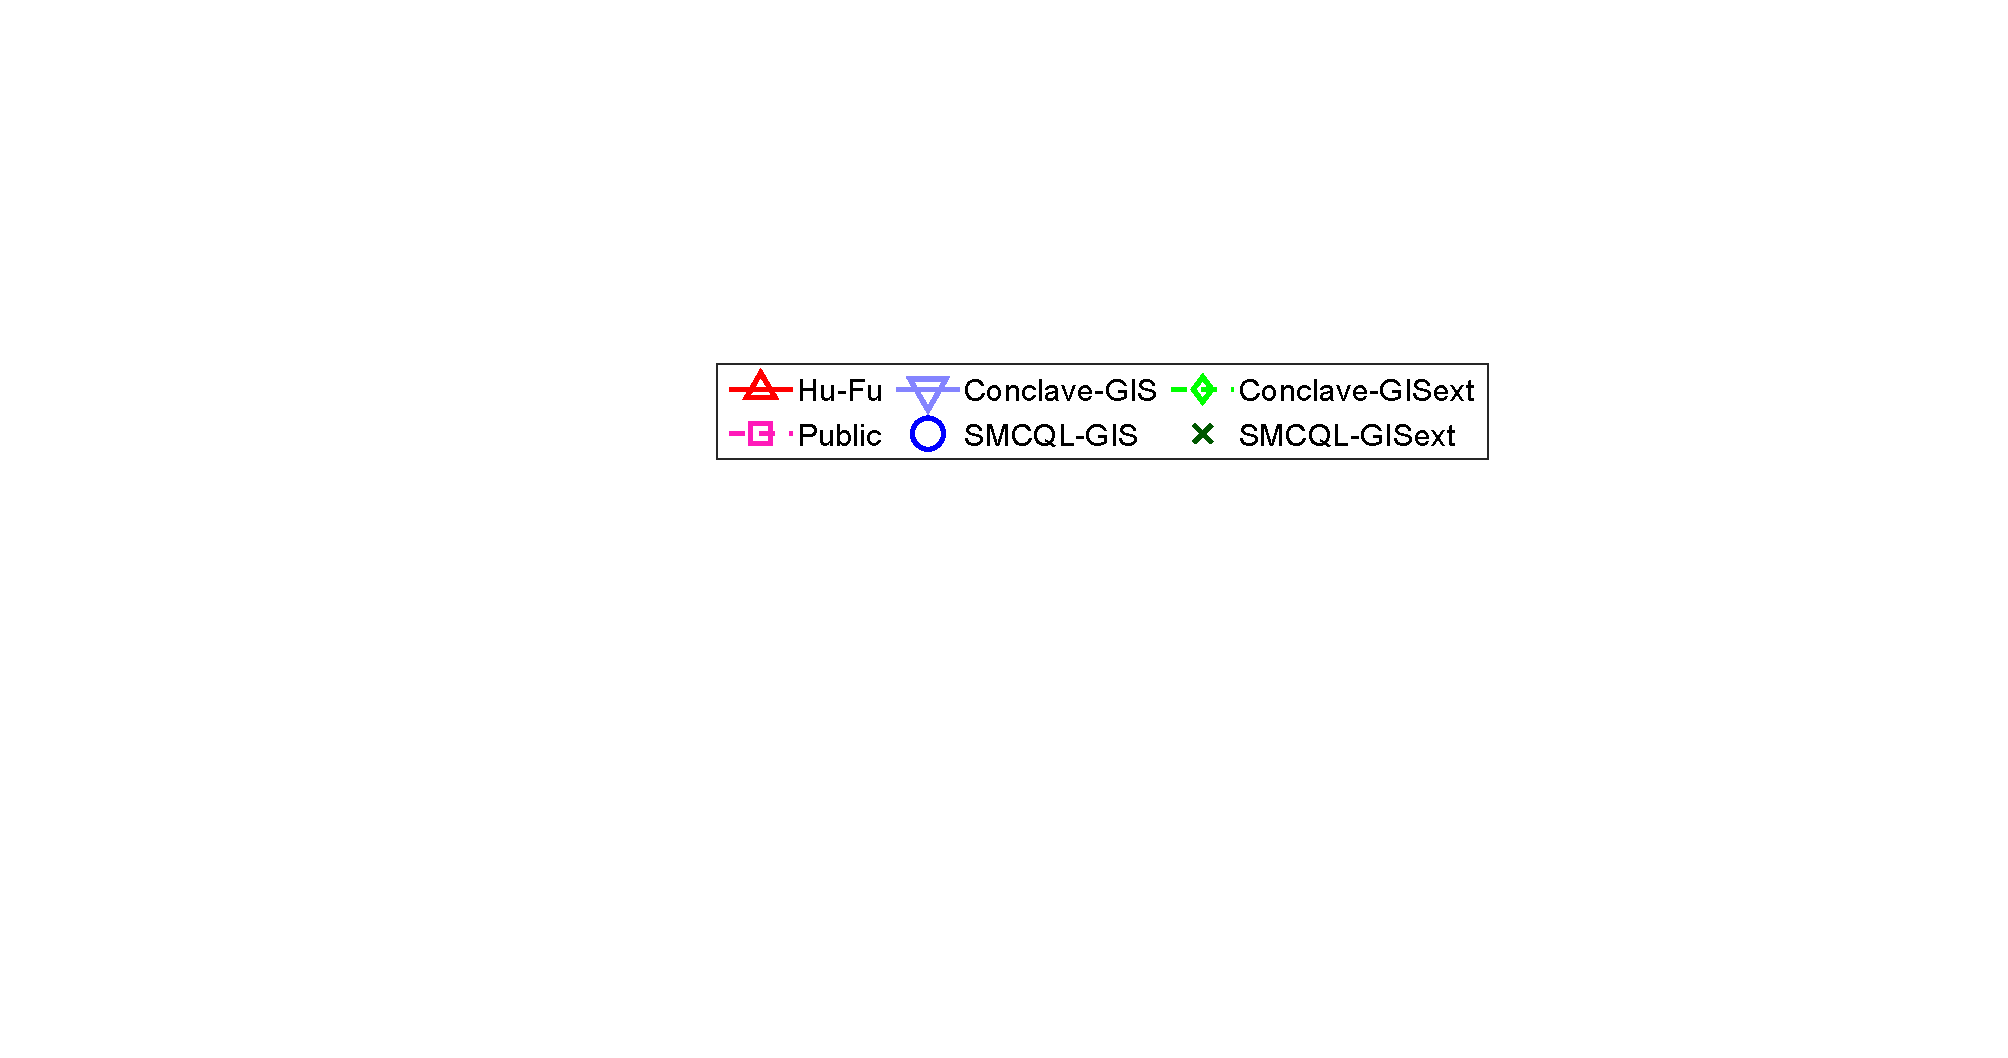
\includegraphics[width=\textwidth]{legend.pdf}
    \end{subfigure}
    \begin{subfigure}{0.48\textwidth}
        \centering
        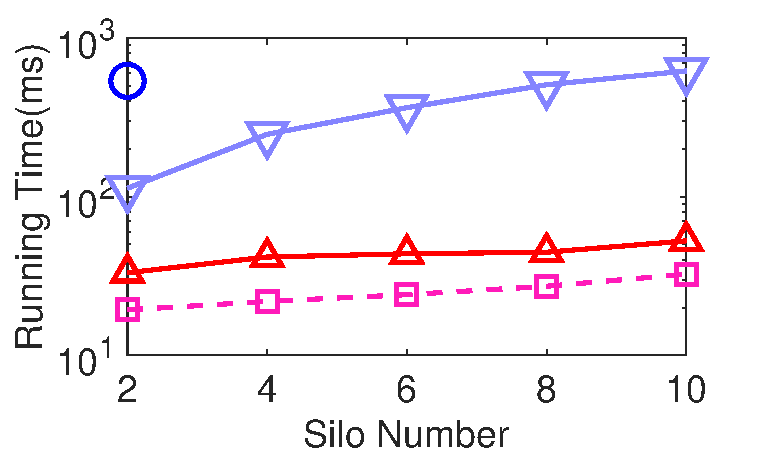
\includegraphics[width=0.48\linewidth]{rangecount_silo_time.pdf}
        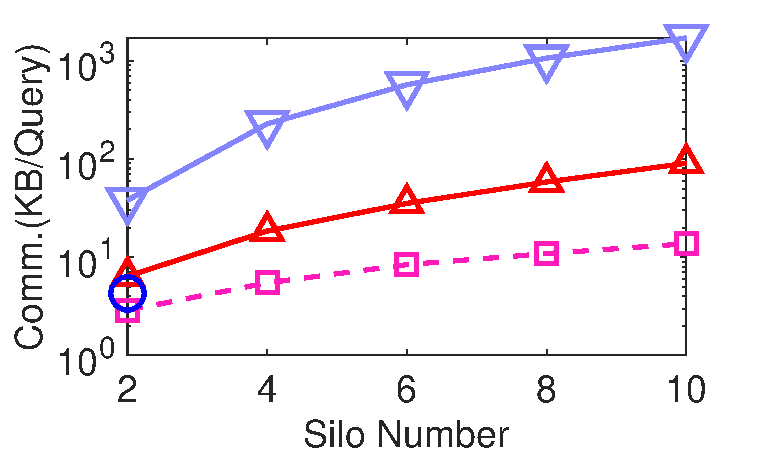
\includegraphics[width=0.48\linewidth]{rangecount_silo_cost.pdf}
        \caption{Runtime and communication cost of varying silo number}
        \label{fig:count-eff-r-n}
    \end{subfigure}
    
    \begin{subfigure}{0.48\textwidth}
        \centering
        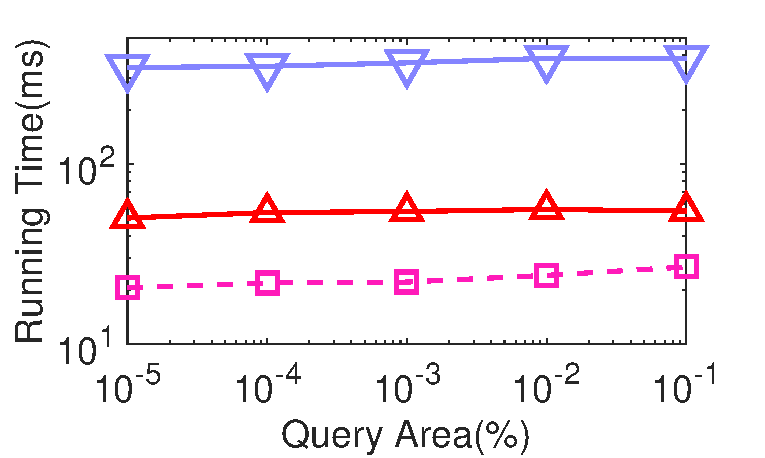
\includegraphics[width=0.48\linewidth]{rangecount_area_time.pdf}
        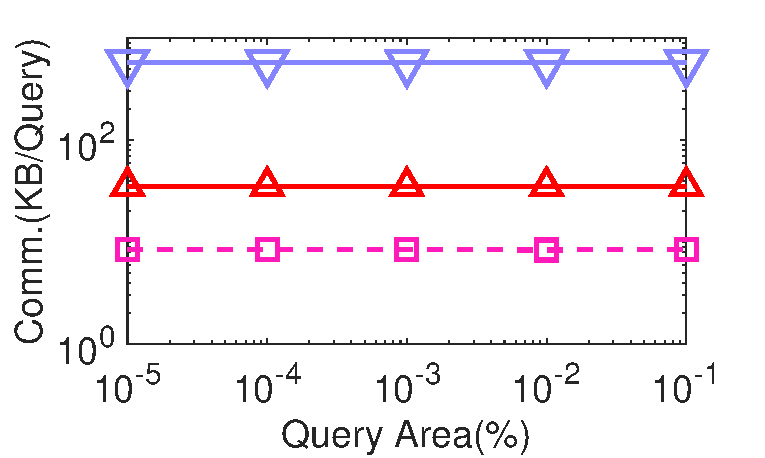
\includegraphics[width=0.48\linewidth]{rangecount_area_cost.pdf}
        \caption{Runtime and communication cost of varying query area}
        \label{fig:count-eff-r-area}
    \end{subfigure}
    \caption{Performance of federated range counting.}
    \label{fig:count-eff}
\end{figure}

\subsubsection{Performance of Federated Range Counting}
\label{sec:exp-asym-rc}

\figref{fig:count-eff} shows the results of (asymmetric) federated range counting.
This query only returns the counting result and thus does not need a secure set union to protect data ownership.
Hence, we exclude \smcqlext and \conclaveext since they only differ from \smcql and \conclave with an extra secure set union, which is unnecessary in this query.
\sysname is up to $15.2\times$ faster than \smcql with a slightly higher communication cost (within 7 KB). 
Considering the increasing network bandwidth, the gap in communication cost is acceptable.
Compared with \conclave, \sysname is up to $10.8 \times$ faster with $17.9 \times$ lower communication cost.
The running time and communication cost of \sysname increase by $0.6 \times$ and $13.2 \times$ respectively when silo number increases to $10$, mainly due to the secure summation.

We also demonstrate the impact of the query area on query efficiency in \figref{fig:count-eff-r-area}.
As is shown, the running time of all methods is relatively stable. 
It is expected because secure operations are the bottleneck of running time whereas the larger query area only increases the running time of plaintext operations.

\begin{figure}[t]
    \centering
    \begin{subfigure}{0.30\textwidth}
        \centering
        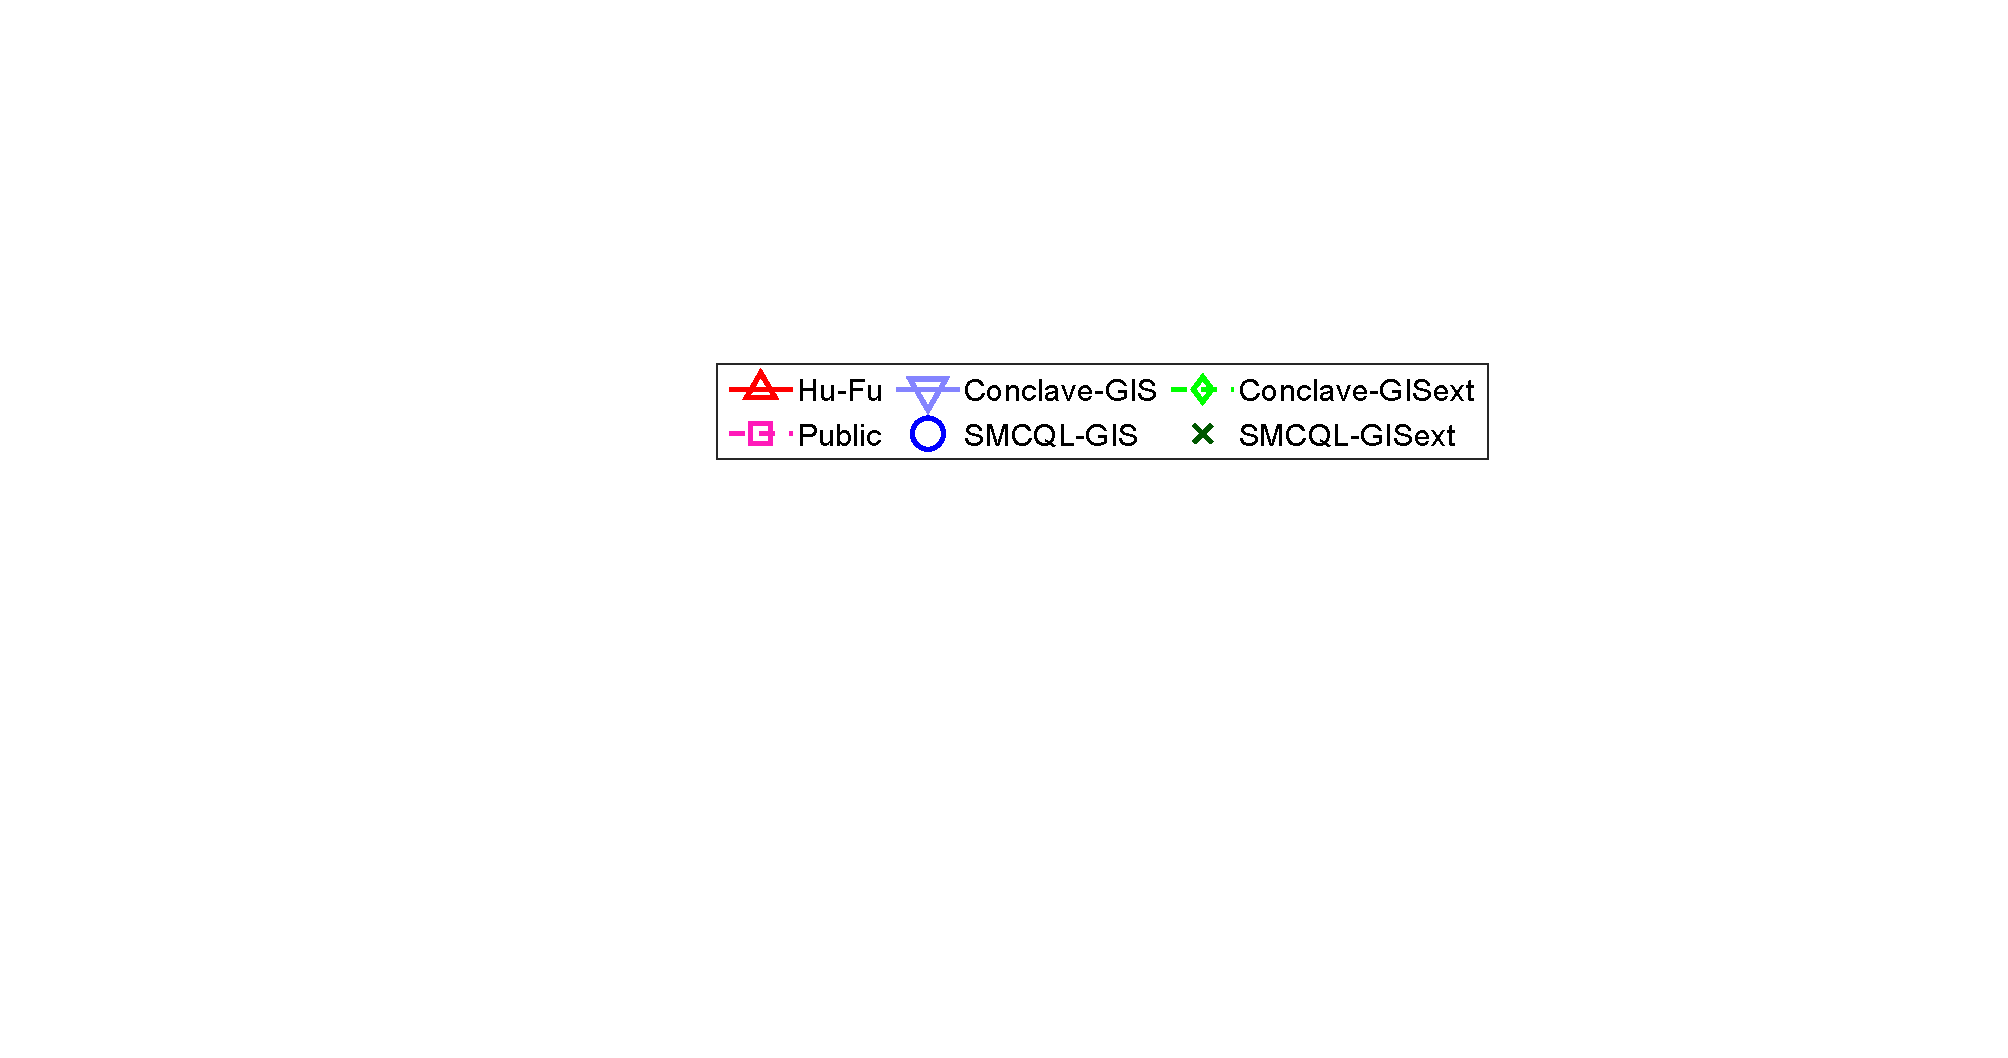
\includegraphics[width=\textwidth]{legend.pdf}
    \end{subfigure}
    
    \begin{subfigure}{0.48\textwidth}
        \centering
        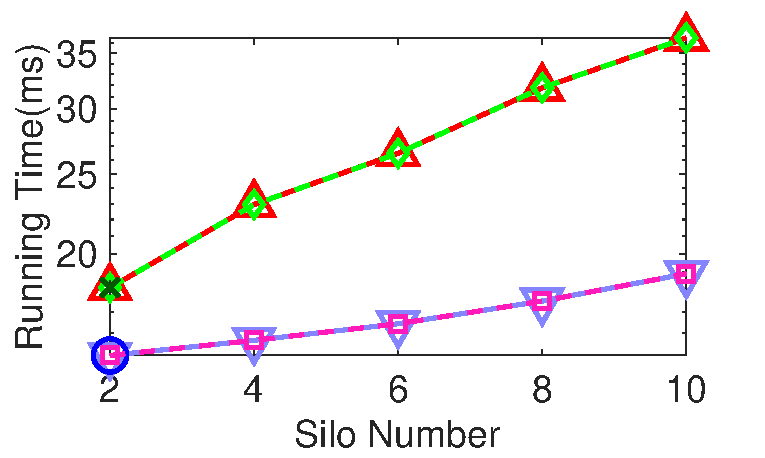
\includegraphics[width=0.48\linewidth]{rangequery_silo_time.pdf}
        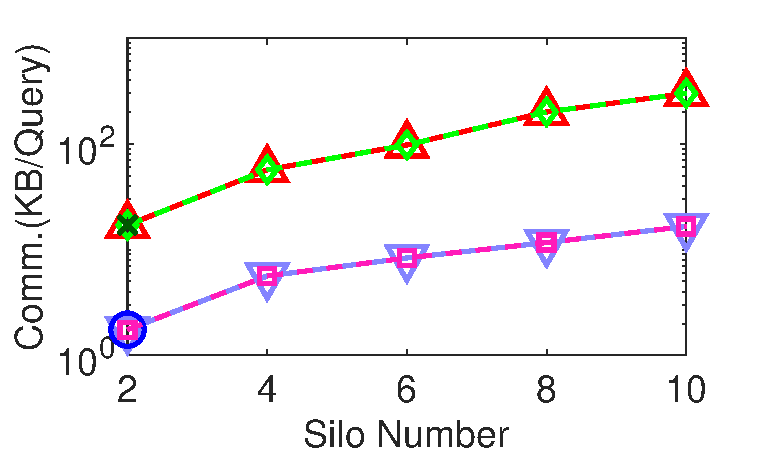
\includegraphics[width=0.48\linewidth]{rangequery_silo_cost.pdf}
        \caption{Runtime and communication cost of varying silo number}
        \label{fig:range-eff-silo-n}
    \end{subfigure}
    \begin{subfigure}{0.48\textwidth}
        \centering
        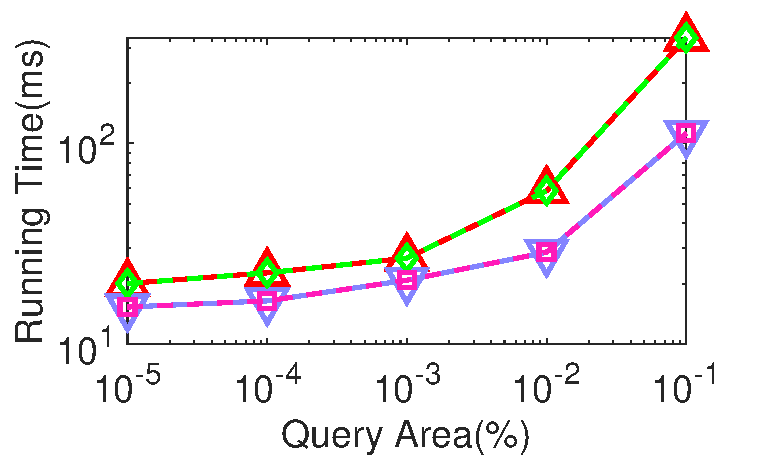
\includegraphics[width=0.48\linewidth]{rangequery_area_time.pdf}
        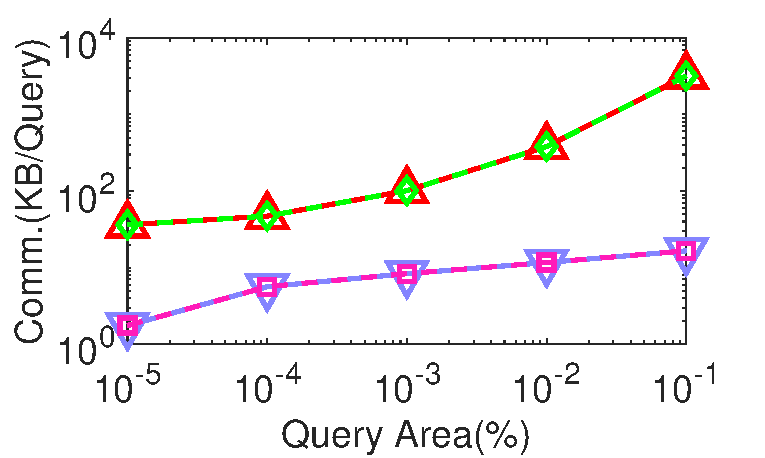
\includegraphics[width=0.48\linewidth]{rangequery_area_cost.pdf}
        \caption{Runtime and communication cost of varying query area}
        \label{fig:range-eff-r-n}
    \end{subfigure}
    \caption{Performance of federated range query.}
    \label{fig:range-eff}
\end{figure}

\subsubsection{Performance of Federated Range Query}
\label{sec:exp-asym-rq}

\figref{fig:range-eff} illustrates the results of (asymmetric) federated range query.
The efficiency of \smcql and \conclave is the same as Public (\ie the non-secure baseline), because they both rely on an honest broker to securely collect partial answers in each silo without leaking them to any others. Under this assumption, all systems can be reduced to Public, which uses a server (\eg an honest broker in \smcql and a center server in Public) to directly collect local range query result from each silo. For example, \sysname with an honest broker also has the same efficiency as Public (see \appref{app:exp-hb}). 

Under a more general setting without this assumption, \sysname, \smcqlext and \conclaveext have the same efficiency because they all use our secure set union for results assembling.
The usage of secure set union only leads to a marginal increase in running time (within $250$ ms) and communication cost (lower than 3.1 MB) over Public.
Note that the order of increase in running time and communication cost matches the complexity analysis for the secure set union in \secref{sec:secure-primitives}, which grows linearly with the silo number and the size of data returned.
As shown in \figref{fig:range-eff-r-n}, when the query area expands, all methods have a higher running time and communication cost, due to the increase of the number of spatial objects in the final result.

\begin{figure}[t]
    \centering
    \begin{subfigure}{0.30\textwidth}
        \centering
        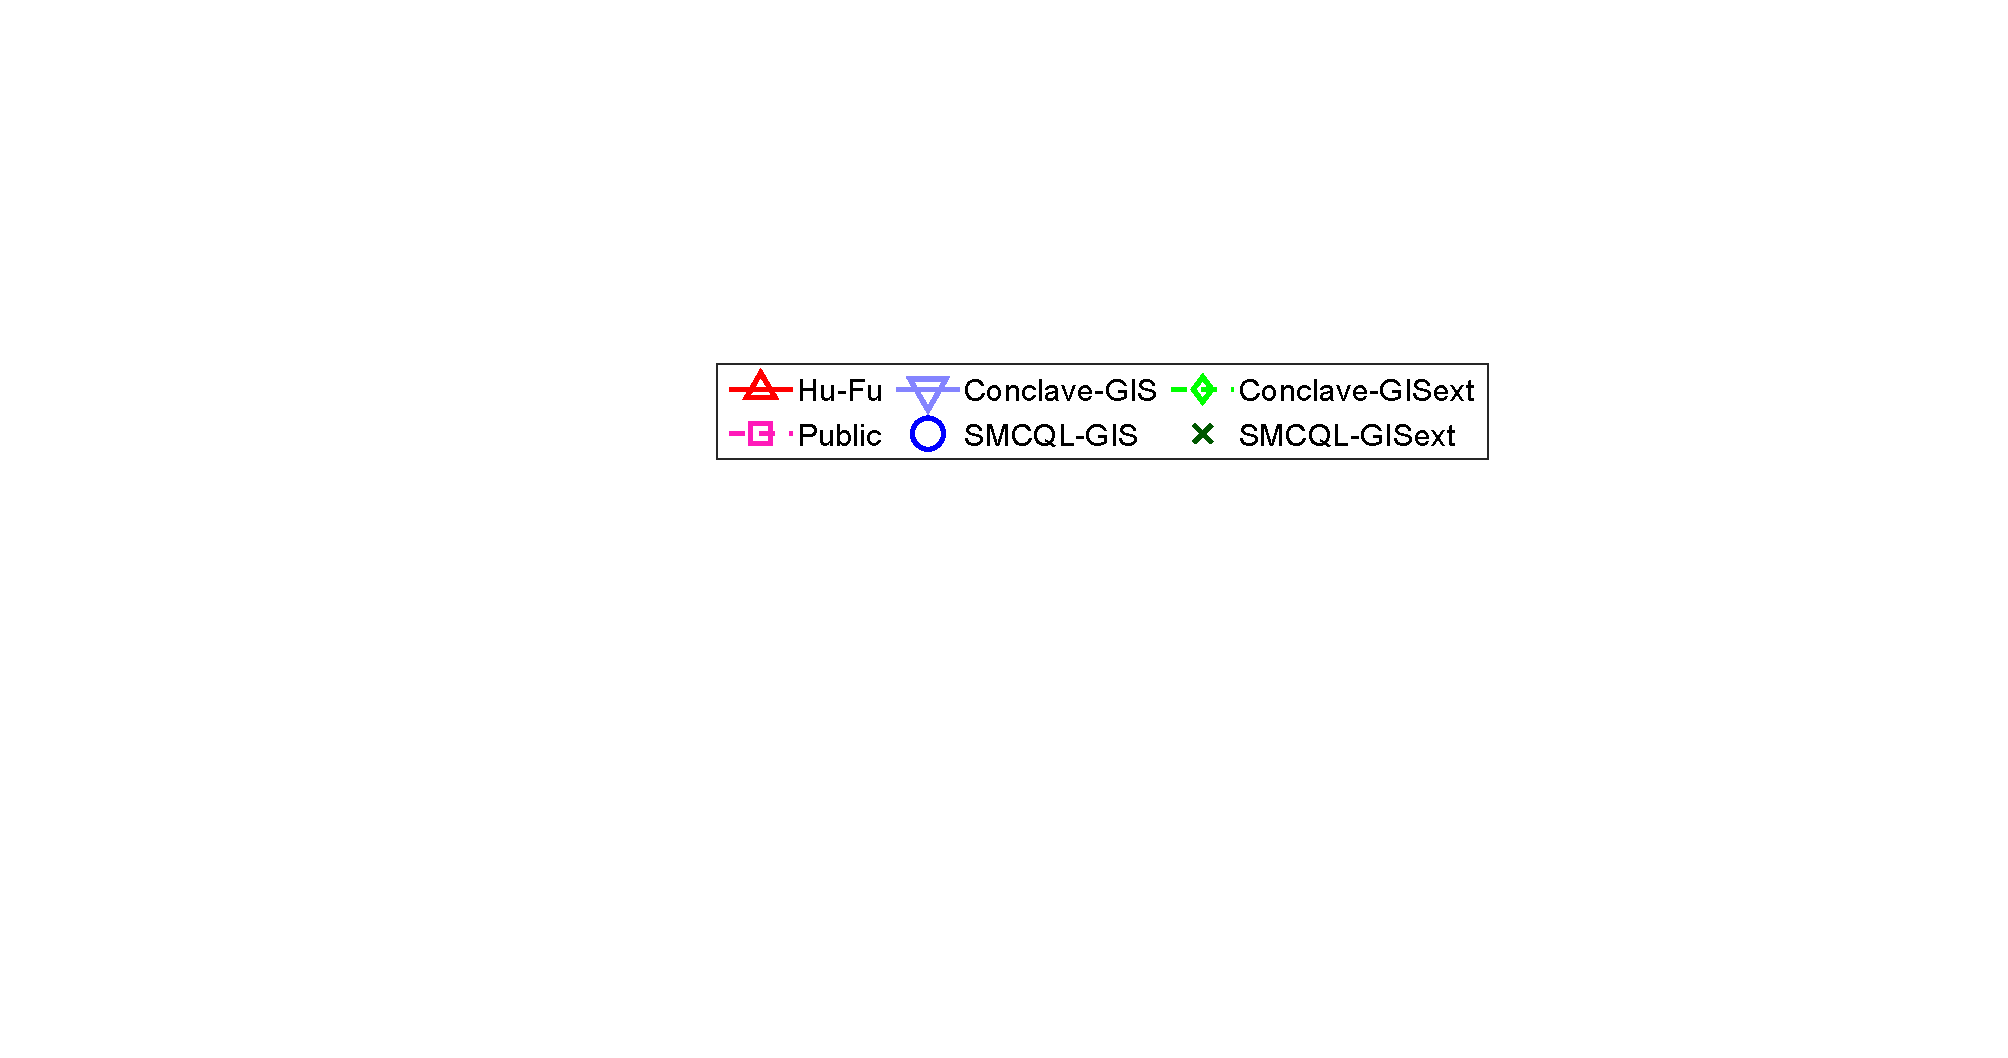
\includegraphics[width=\textwidth]{legend.pdf}
    \end{subfigure}
    \begin{subfigure}{0.48\textwidth}
        \centering
        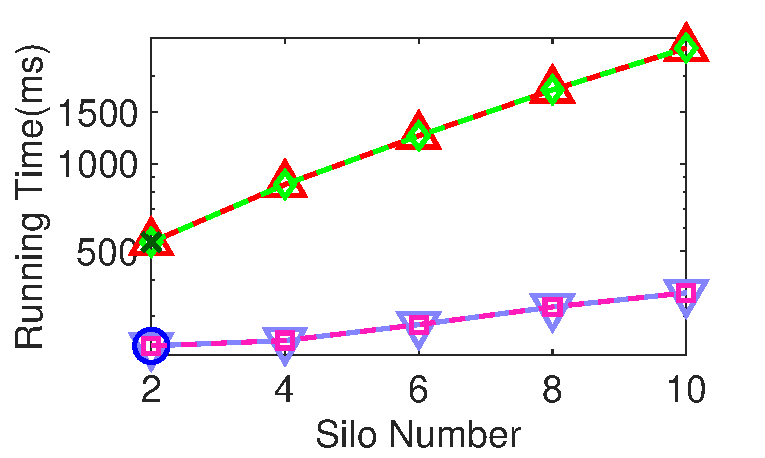
\includegraphics[width=0.48\linewidth]{dj_silo_time.pdf}
        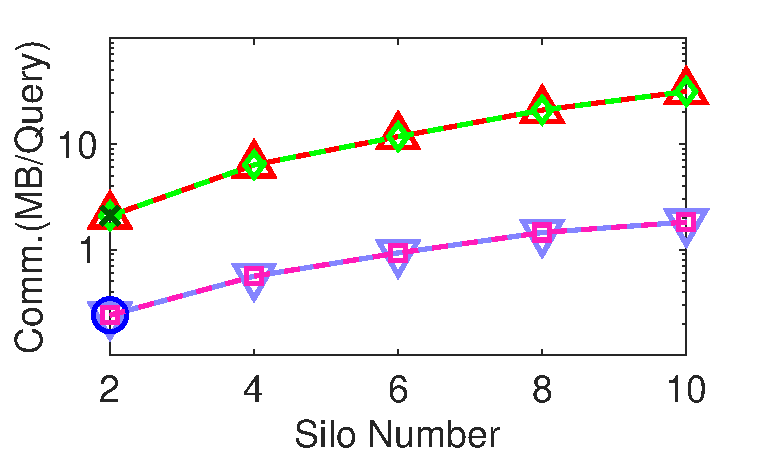
\includegraphics[width=0.48\linewidth]{dj_silo_cost.pdf}
        \caption{Runtime and communication cost of varying silo number}
        \label{fig:djoin-eff-silo-n}
    \end{subfigure}
    
    \begin{subfigure}{0.48\textwidth}
        \centering
        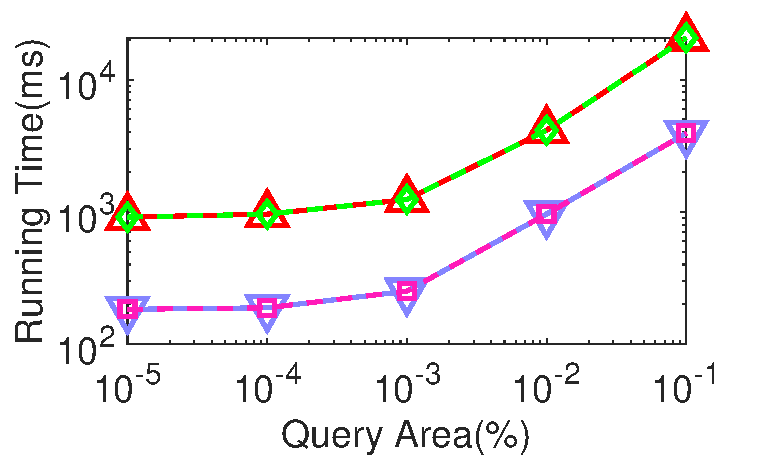
\includegraphics[width=0.48\linewidth]{dj_area_time.pdf}
        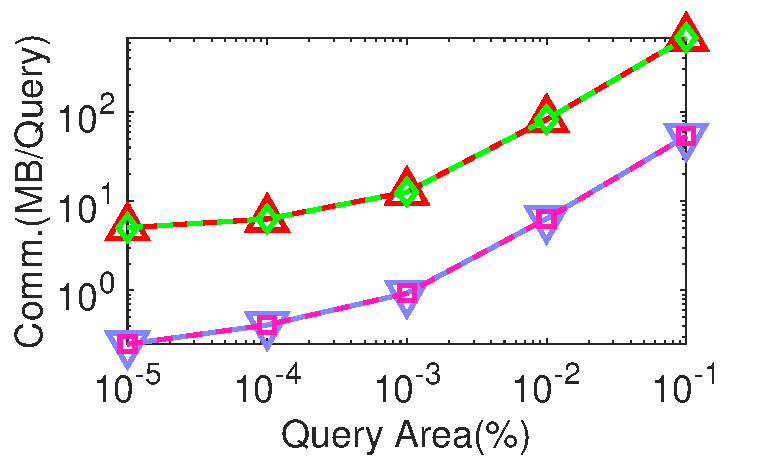
\includegraphics[width=0.48\linewidth]{dj_area_cost.pdf}
        \caption{Runtime and communication cost of varying query area}
        \label{fig:djoin-eff-r-n}
    \end{subfigure}
    \caption{Performance of federated distance join.}
    \label{fig:dis-join-eff}
\end{figure}

\subsubsection{Performance of Federated Distance Join}
\label{sec:exp-asym-rqj}

\figref{fig:dis-join-eff} presents the performance of (asymmetric) federated distance join. 
Note that all the methods treat federated distance join as multiple independent federated range queries, where the total number of these range queries is $|R|=100$ in this test.
Thus, it is reasonable that the ranking of all the methods is similar to that in federated range query (see \figref{fig:range-eff}).
The result of federated distance join when varying the query area shows a similar pattern with that of federated range query. 
This is because a federated distance join is decomposed into multiple federated range queries for all the compared solutions.
The increase of both running time and communication cost is caused by the increase of the number of retrieved spatial objects.

\subsubsection{Summary of Major Findings}
\label{sec:exp-asym-summary}

We have observed the following findings in the experiments of asymmetric queries.
\begin{itemize}
    \item \sysname is up to $15,814.2\times$ faster than \smcql and \conclave, with up to $5$ orders of magnitude lower communication cost.
    The efficiency gain of \sysname over the baselines is more notable in federated kNN query, kNN join, and range counting, which is at least $2.4\times$ faster in time cost and $4.9\times$ lower in communication cost than \conclave.
    
    \item \smcql and \conclave are more efficient in federated range query and distance join,
    because these baselines are reduced to Public and need no secure operation with the honest broker.
    Note that for federated range query and distance join, \sysname achieves the same efficiency as \smcqlext and \conclaveext, the variants of \smcql and \conclave without an honest broker. 
    
    \item The experimental trends of federated kNN join and distance join are similar to those of federated kNN query and range query for all compared solutions.
    This is reasonable since a federated kNN join or distance join is decomposed into a series of federated kNN queries or range queries.
\end{itemize}

\subsection{Experiments on Symmetric Queries}
\label{subsec:exp-symmetric}

\fakeparagraph{Parameter Setting}
The parameter configurations for the query workloads are identical to those introduced in Section \ref{subsec:exp-cmp}.
\rev{Beyond these parameters, the privacy budget $\epsilon$ also affects the query performance of \sysname.
In general, a smaller $\epsilon$ (\ie stricter privacy preservation) leads to lower efficiency than a larger $\epsilon$.
Please refer to \appref{app:budget} for the evaluation of varying $\epsilon$ in \sysname.}
We have omitted reporting the results of the federated kNN join,
since the query efficiency of \sysname's federated kNN join can be inferred from the results of its federated kNN query, as evidenced by previous experiments.
We also omit the results of \smcql, \smcqlext, and \conclaveext, since their results are similar to \conclave when answering symmetric queries.
Additional baselines, \EDBT \cite{DBLP:conf/edbt/KesarwaniKNPSMM18} and \ICDE \cite{DBLP:conf/icde/SahinAAAP18}, are involved in this experiment, where \ICDE is limited to federated range query and distance join.

\fakeparagraph{Environment}
\rev{Due to the expired funding support, the hardware environment for testing asymmetric queries is no longer accessible,
so all solutions to symmetric queries are tested in a new hardware environment.}
Specifically, this new environment is composed of 5 cloud servers. 
Each server has Intel Xeon(R) Platinum 8361HC CPU 2.60GHZ processors and 32GB memory with Ubuntu 18.04 LTS OS.
The network bandwidth between servers is up to 1.5 GB/s and may fluctuate slightly at different times.
Four of the five servers act as data silos. 
Since this experiment requires up to 10 data silos, each of these four servers can host up to 3 data silos using different processes.
The remaining server is only used as the user's client, facilitating parallel data transmission between data silos for compare solutions.
\rev{For each query type, we generate 50 queries, repeat 10 times for each query, and report the average results.}

% In the following, we present the experimental results and analysis of the federated range counting, range query, distance join, and kNN query in \secref{sec:exp-symm-rc} to \secref{sec:exp-symm-knn}, respectively.
% Finally, we summarize the major findings in \secref{sec:exp-symm-summary}.

\begin{figure}[t]
    \centering
    \begin{subfigure}{0.48\textwidth}
        \centering
        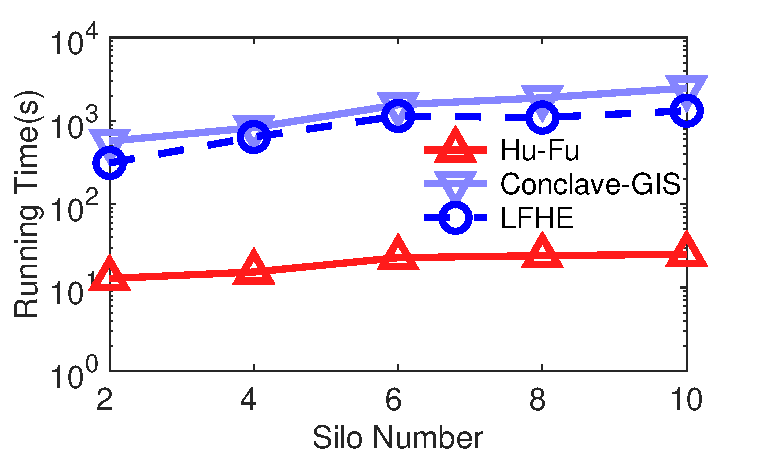
\includegraphics[width=0.48\linewidth]{traffic_rangecount_silo_time.pdf}
        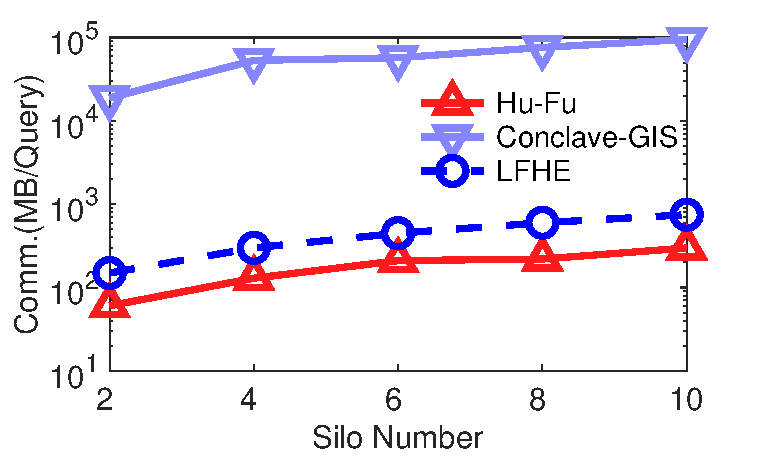
\includegraphics[width=0.48\linewidth]{traffic_rangecount_silo_comm.pdf}
        \caption{Runtime and communication cost of varying silo number}
        \label{fig:symmetric-count-eff-silo-n}
    \end{subfigure}
    \begin{subfigure}{0.48\textwidth}
        \centering
        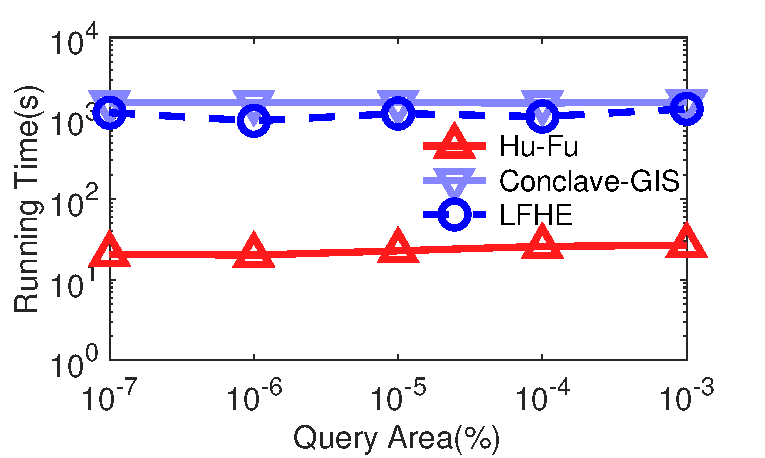
\includegraphics[width=0.48\linewidth]{traffic_rangecount_area_time.pdf}
        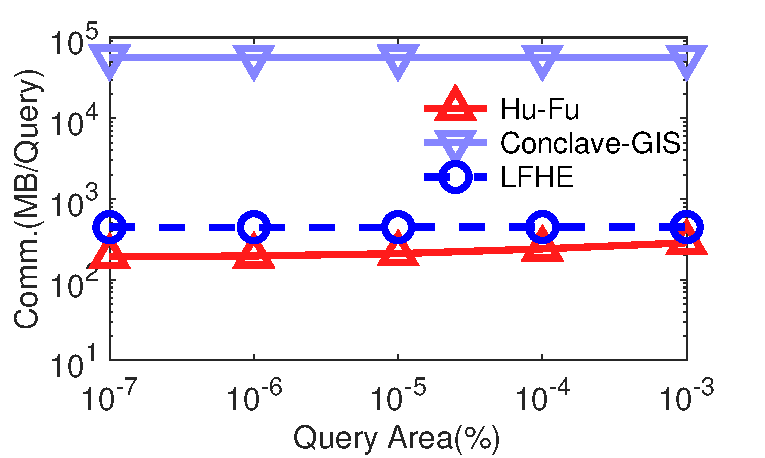
\includegraphics[width=0.48\linewidth]{traffic_rangecount_area_comm.pdf}
        \caption{Runtime and communication cost of varying query area}
        \label{fig:symmetric-count-eff-r-n}
    \end{subfigure}
    \caption{Performance of federated range counting.}
    \label{fig:symmetric-count-eff}
\end{figure}

\subsubsection{Performance of Federated Range Counting}
\label{sec:exp-symm-rc}

\rev{\figref{fig:symmetric-count-eff} shows the results of (symmetric) federated range counting. 
\sysname always outperforms the compared baselines in both running time and communication cost.
\sysname takes up to 98.9$\times$ shorter runtime and up to 410.7$\times$ lower communication cost than \conclave. 
\sysname is also up to 56.6$\times$ faster with up to 2.7$\times$ lower communication cost compared to \EDBT.}

\rev{We can also observe that as the silo number increases from 2 to 10, 
the running time and communication cost of all compared algorithms tend to increase. 
This pattern is reasonable, as more data silos require more secure computations among them. 
When the query area expands from small to large, the runtime and communication overhead of \sysname increase slightly. 
This trend in \sysname is attributable to the increase of candidates for secure distance comparisons.}
% When comparing the experimental results for asymmetric federated range counting in \figref{fig:count-eff}, we can observe a substantial increase in both running time and communication cost for either \sysname or \conclave.
% This increase is due to the inevitable usage of secure distance-related operators for symmetric queries.
% This observation also indicates that symmetric queries, which demand additional consideration for query privacy, are more challenging than asymmetric queries.

\begin{figure}[t]
    \centering
    \begin{subfigure}{0.48\textwidth}
        \centering
        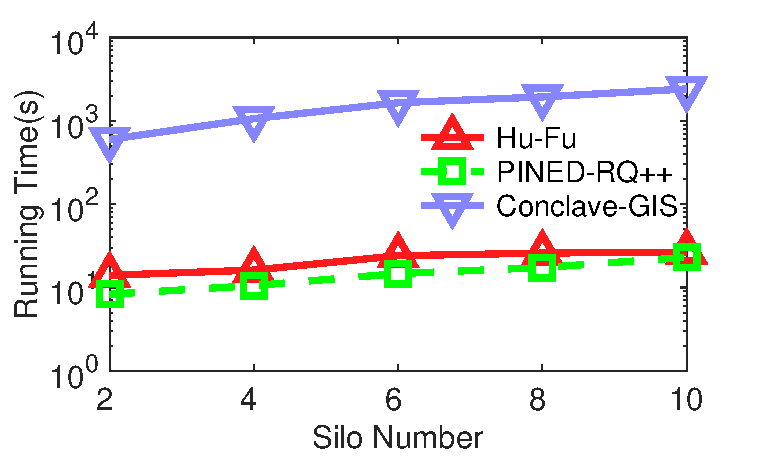
\includegraphics[width=0.48\linewidth]{traffic_rangequery_silo_time.pdf}
        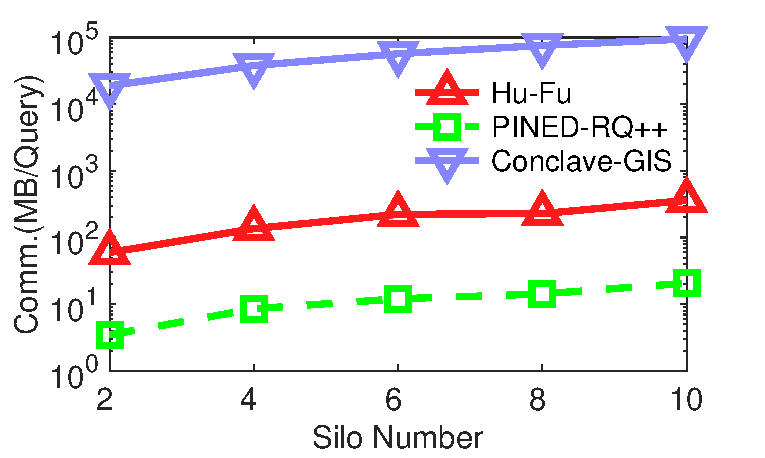
\includegraphics[width=0.48\linewidth]{traffic_rangequery_silo_comm.pdf}
        \caption{Runtime and communication cost of varying silo number}
        \label{fig:symmetric-range-eff-silo-n}
    \end{subfigure}
    \begin{subfigure}{0.48\textwidth}
        \centering
        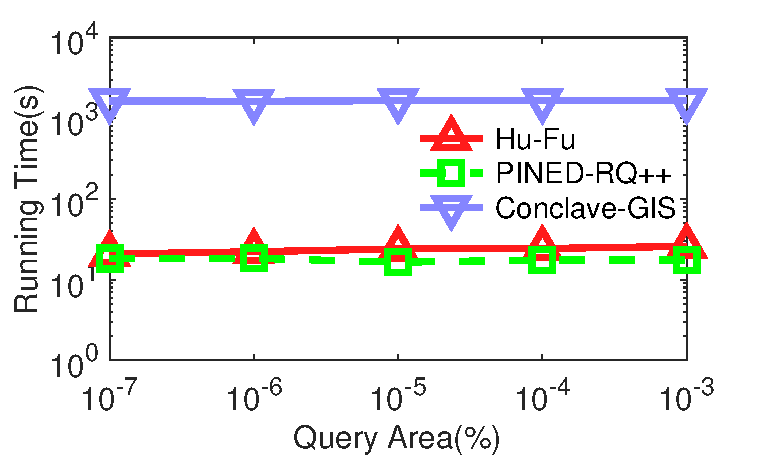
\includegraphics[width=0.48\linewidth]{traffic_rangequery_area_time.pdf}
        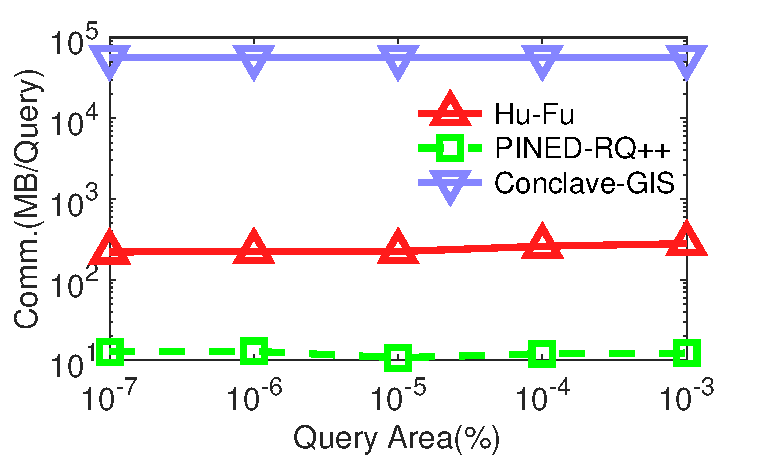
\includegraphics[width=0.48\linewidth]{traffic_rangequery_area_comm.pdf}
        \caption{Runtime and communication cost of varying query area}
        \label{fig:symmetric-range-eff-r-n}
    \end{subfigure}
    \caption{Performance of federated range query.}
    \label{fig:symmetric-range-eff}
\end{figure}

\subsubsection{Performance of Federated Range Query}
\label{sec:exp-symm-rq}

\figref{fig:symmetric-range-eff} illustrates the performance of (symmetric) federated range queries. 
\rev{The results of \EDBT are not reported because the running time is over 1 hour and the memory consumption exceeds the server configuration (32 GB).
In fact, \EDBT can only handle a small-scale dataset. For example, \EDBT already takes 13 minutes and 3 MB of communication cost when the data size is $10^4$.
Although \ICDE is more efficient than \sysname and \conclave, it suffers from \textit{two major drawbacks}: (1) it leaks locations of the candidate data objects that are not part of the true answer to the query user and (2) it is only capable of retrieving approximation results.
For example, the recall of \ICDE is \rev{72.8\%-96.8\%} when varying the silo number and \rev{72.2\%-92.3\%} when varying the query area.}

Aside from \ICDE, \sysname achieves the best performance in the efficiency and security. 
It takes at least 42.7$\times$ shorter time with at least 204.2$\times$ lower communication cost compared to \conclave.
\rev{\figref{fig:symmetric-range-eff} exhibits a similar trend in the efficiency variation of \sysname when comparing to the results in \figref{fig:symmetric-count-eff} (for federated range counting). 
This similarity arises because the query decomposition plans for symmetric federated range queries and counting are quite identical. 
The main difference lies in the additional secure set union operator required for federated range queries.}
% \rev{As shown in \figref{fig:symmetric-range-eff-silo-n}, 
% the efficiency of all methods remains consistent despite increases in the numbers of silos, as the overall data size remains unchanged. 
% Due to the parallel processing of the \sysname architecture, running time decreases as the data size of each individual silo decreases. 
% In addition, we further elucidate the effect of the query area on the query efficiency in \figref{fig:symmetric-range-eff-r-n}.}


\begin{figure}[t]
    \centering
    \begin{subfigure}{0.48\textwidth}
        \centering
        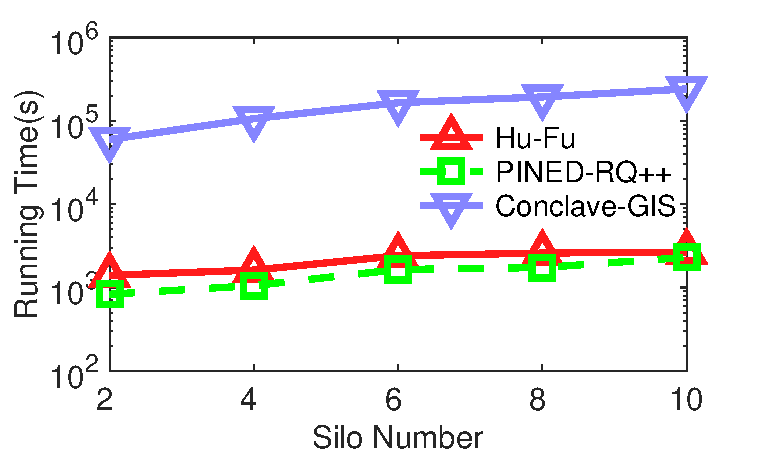
\includegraphics[width=0.48\linewidth]{traffic_join_silo_time.pdf}
        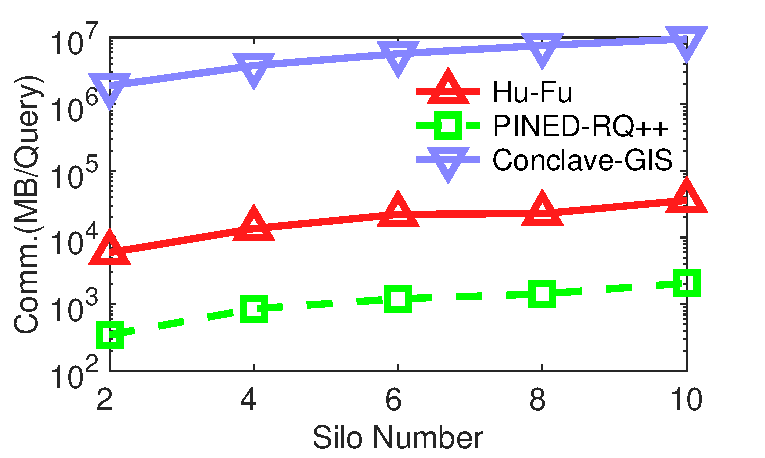
\includegraphics[width=0.48\linewidth]{traffic_join_silo_comm.pdf}
        \caption{Runtime and communication cost of varying silo number}
        \label{fig:symmetric-join-eff-silo-n}
    \end{subfigure}
    \begin{subfigure}{0.48\textwidth}
        \centering
        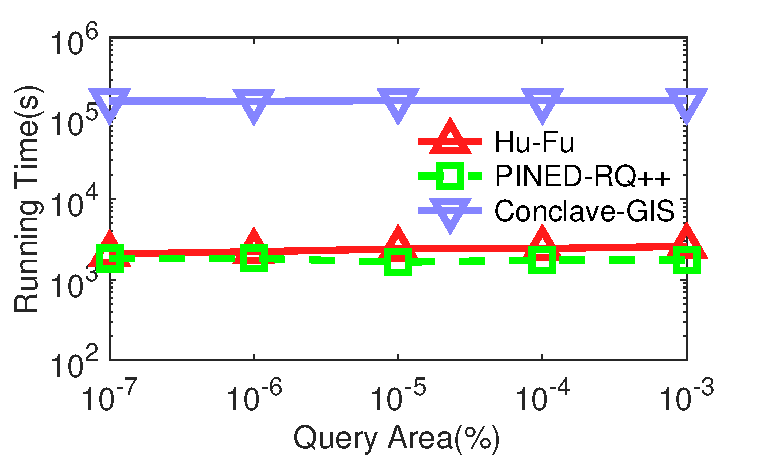
\includegraphics[width=0.48\linewidth]{traffic_join_area_time.pdf}
        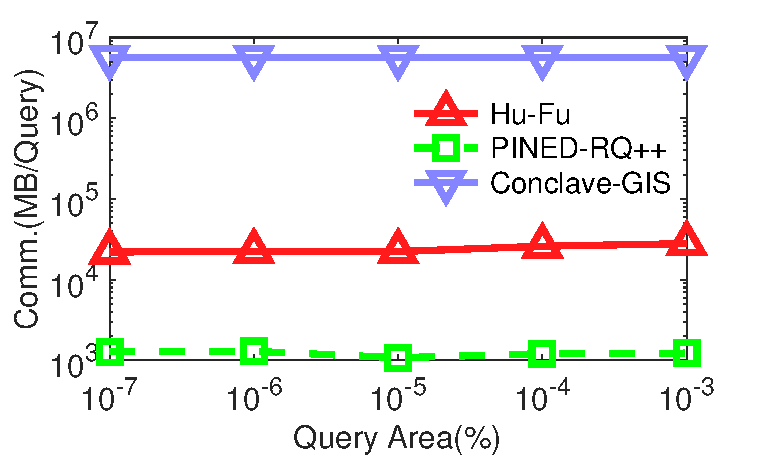
\includegraphics[width=0.48\linewidth]{traffic_join_area_comm.pdf}
        \caption{Runtime and communication cost of varying query area}
        \label{fig:symmetric-join-eff-r-n}
    \end{subfigure}
    \caption{Performance of federated distance join.}
    \label{fig:symmetric-join-eff}
\end{figure}

\subsubsection{Performance of Federated Distance Join}
\label{sec:exp-symm-djoin}

\figref{fig:symmetric-join-eff} presents the performance of (symmetric) federated distance joins. 
Here, a symmetric federated distance join employs the same strategy as the asymmetric federated distance join, treating the join operation as multiple independent federated range queries, with $|R|=100$. Therefore, the relative performance of all methods here is similar to that of symmetric federated range query (see \figref{fig:symmetric-range-eff}). 
Compared with \ICDE, although \sysname incurs higher communication cost, it takes nearly the same amount of running time and offers a more secure solution that produces the exact query answer. 
\rev{Compared to \conclave, \sysname is up to 90.7$\times$ faster and up to 332.5$\times$ lower in communication cost.}
By contrast, \EDBT is the least efficient method and cannot respond to a join query within 6 hours, so we cannot report its result in \figref{fig:symmetric-join-eff}.

\begin{figure}[t]
    \centering
    \begin{subfigure}{0.48\textwidth}
        \centering
        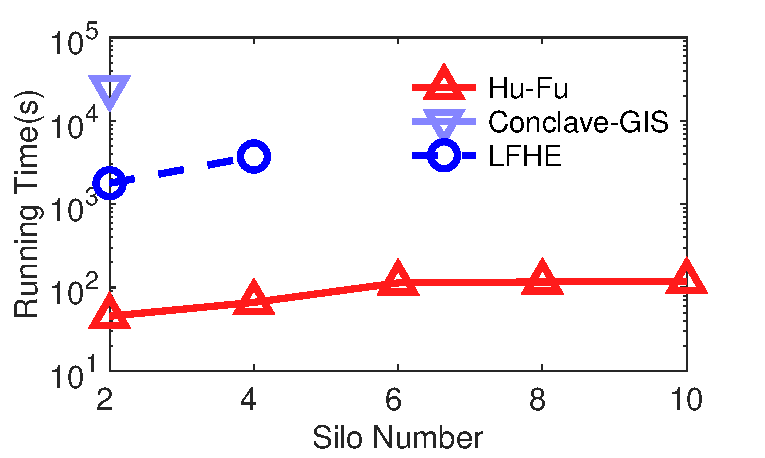
\includegraphics[width=0.48\linewidth]{traffic_knn_silo_time.pdf}
        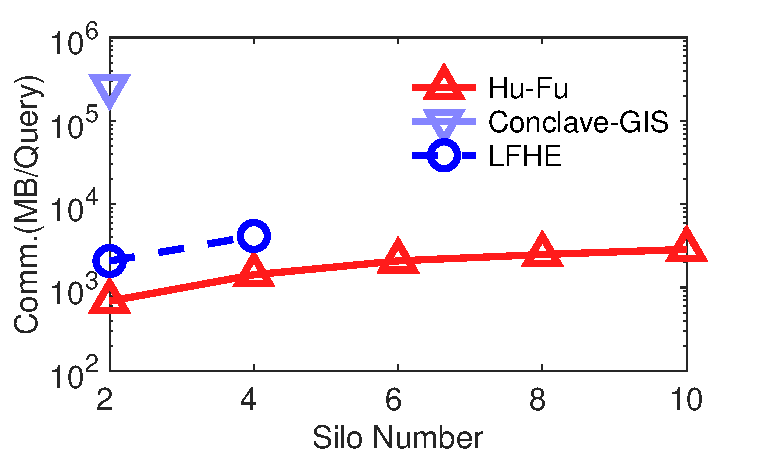
\includegraphics[width=0.48\linewidth]{traffic_knn_silo_comm.pdf}
        \caption{Runtime and communication cost of varying silo number}
        \label{fig:symmetric-knn-eff-silo-n}
    \end{subfigure}
    \begin{subfigure}{0.48\textwidth}
        \centering
        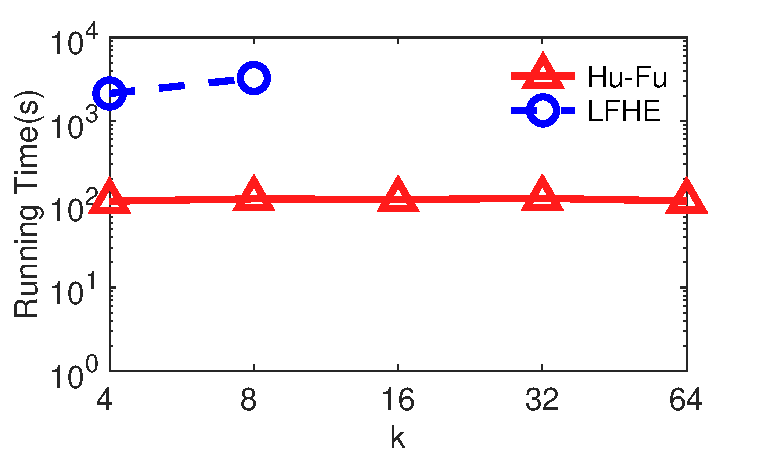
\includegraphics[width=0.48\linewidth]{traffic_knn_k_time.pdf}
        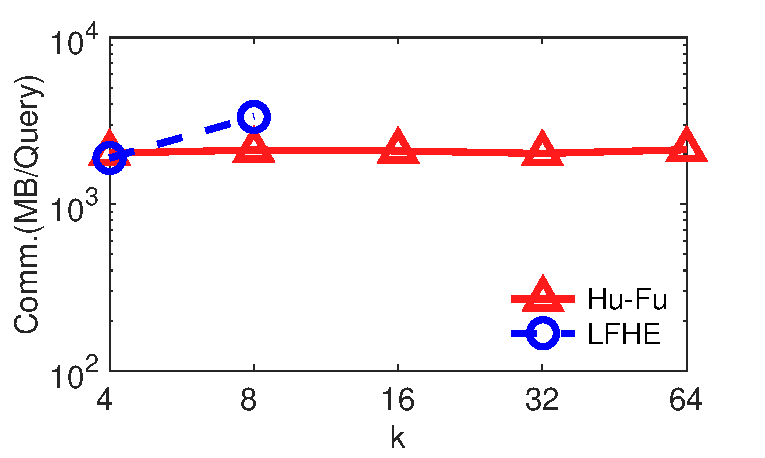
\includegraphics[width=0.48\linewidth]{traffic_knn_k_comm.pdf}
        \caption{Runtime and communication cost of varying $k$}
        \label{fig:symmetric-knn-eff-k}
    \end{subfigure}
    \caption{Performance of federated kNN query.}
    \label{fig:symmetric-knn-eff}
\end{figure}

\subsubsection{Performance of Federated kNN Query}
\label{sec:exp-symm-knn}

\figref{fig:symmetric-knn-eff} shows the running time and communication cost of (symmetric) federated kNN queries. 
We cannot report some results of \EDBT and \conclave because they cannot terminate within 1 hour to process a single query or the maximum memory usage is beyond the limitation (32 GB) of the cloud server. 
Additionally, \ICDE is unable to handle KNN queries, so it is excluded in this evaluation.
According to the experimental results, \sysname is the most efficient solution to federated kNN queries.
\rev{For instance, \sysname is up to 551.8$\times$ faster than \conclave and 56.2$\times$ faster than \EDBT, with up to 380.0$\times$ and 3.0$\times$ lower communication overhead than them, respectively.
Similar to previous results, the time cost of \sysname gradually increases as the silo number increases.
By contrast, the efficiency of \sysname does not notably change as $k$ increases.}

\begin{table}[t]
    \centering  
    \caption{\rev{Improvement with upper bound in \lemref{lem:knn-UB}}}\label{tab:bound-improvement}
    \begin{tabular}{c *{5}{c}}
    \hline  
    $k$ & 4 & 8 & 16 & 32 & 64 \\  
    \hline  
    Running time & 6.3$\times$ & 4.2$\times$ & 4.0$\times$ & 3.6$\times$ & 3.4$\times$ \\  
    Communication & 5.0$\times$ & 3.9$\times$ & 3.6$\times$ & 3.4$\times$ & 3.1$\times$ \\  
    \hline  
    \end{tabular}  
\end{table} 

\rev{We also evaluate the improvement of using the upper bound in \lemref{lem:knn-UB}.
As shown in \tabref{tab:bound-improvement}, 
this optimization improves the running time by up to 6.3$\times$ and reduces the communication cost by up to 5.0$\times$.} 

\subsubsection{Summary of Major Findings}
\label{sec:exp-symm-summary}

The major findings in the experiments of symmetric queries are summarized as follows.
\begin{itemize}
    \item \rev{\sysname is at least 42.7$\times$ faster than \conclave, with at least 204.2$\times$ lower communication overhead.
    Compared to \EDBT, \sysname is up to 56.6$\times$ faster with up to 3.0$\times$ lower communication overhead.}

    \item Although \ICDE is more efficient than the others, it suffers from three significant drawbacks:
    (1) violations on the data privacy,
    (2) inability to provide exact answers,
    and (3) limited support to only federated range queries.
    By contrast, our \sysname can address all these drawbacks effectively.
    
    \item When comparing with the evaluations of asymmetric queries in \secref{subsec:exp-cmp}, it is evident that running time and communication overhead both escalate when \sysname or \conclave processes symmetric queries.
    Consequently, symmetric queries pose a greater challenge than asymmetric queries, primarily due to the additional concern for query privacy.
\end{itemize}

\rev{\fakeparagraph{Remark}
To assess the impact of query privacy on time efficiency, 
we can compare the running time of asymmetric and symmetric queries in the new hardware environment. 
Our evaluation shows that the baseline \conclave takes $4,054$$\times$ longer to protect query privacy in federated range queries, 
while our solution \sysname reduces this gap to $59$$\times$. 
Please see \appref{app:impact-query-privacy} for more detailed results.}

\subsection{Experiments on Scalability Tests}
\label{subsec:exp-scalability}

In the following, we report the results of scalability tests on asymmetric queries and symmetric queries in \secref{subsec:exp-asymm-scalability} and \secref{subsec:exp-symm-scalability}, respectively.

\begin{figure}[t]
    \centering
    \begin{subfigure}{0.30\textwidth}
        \centering
        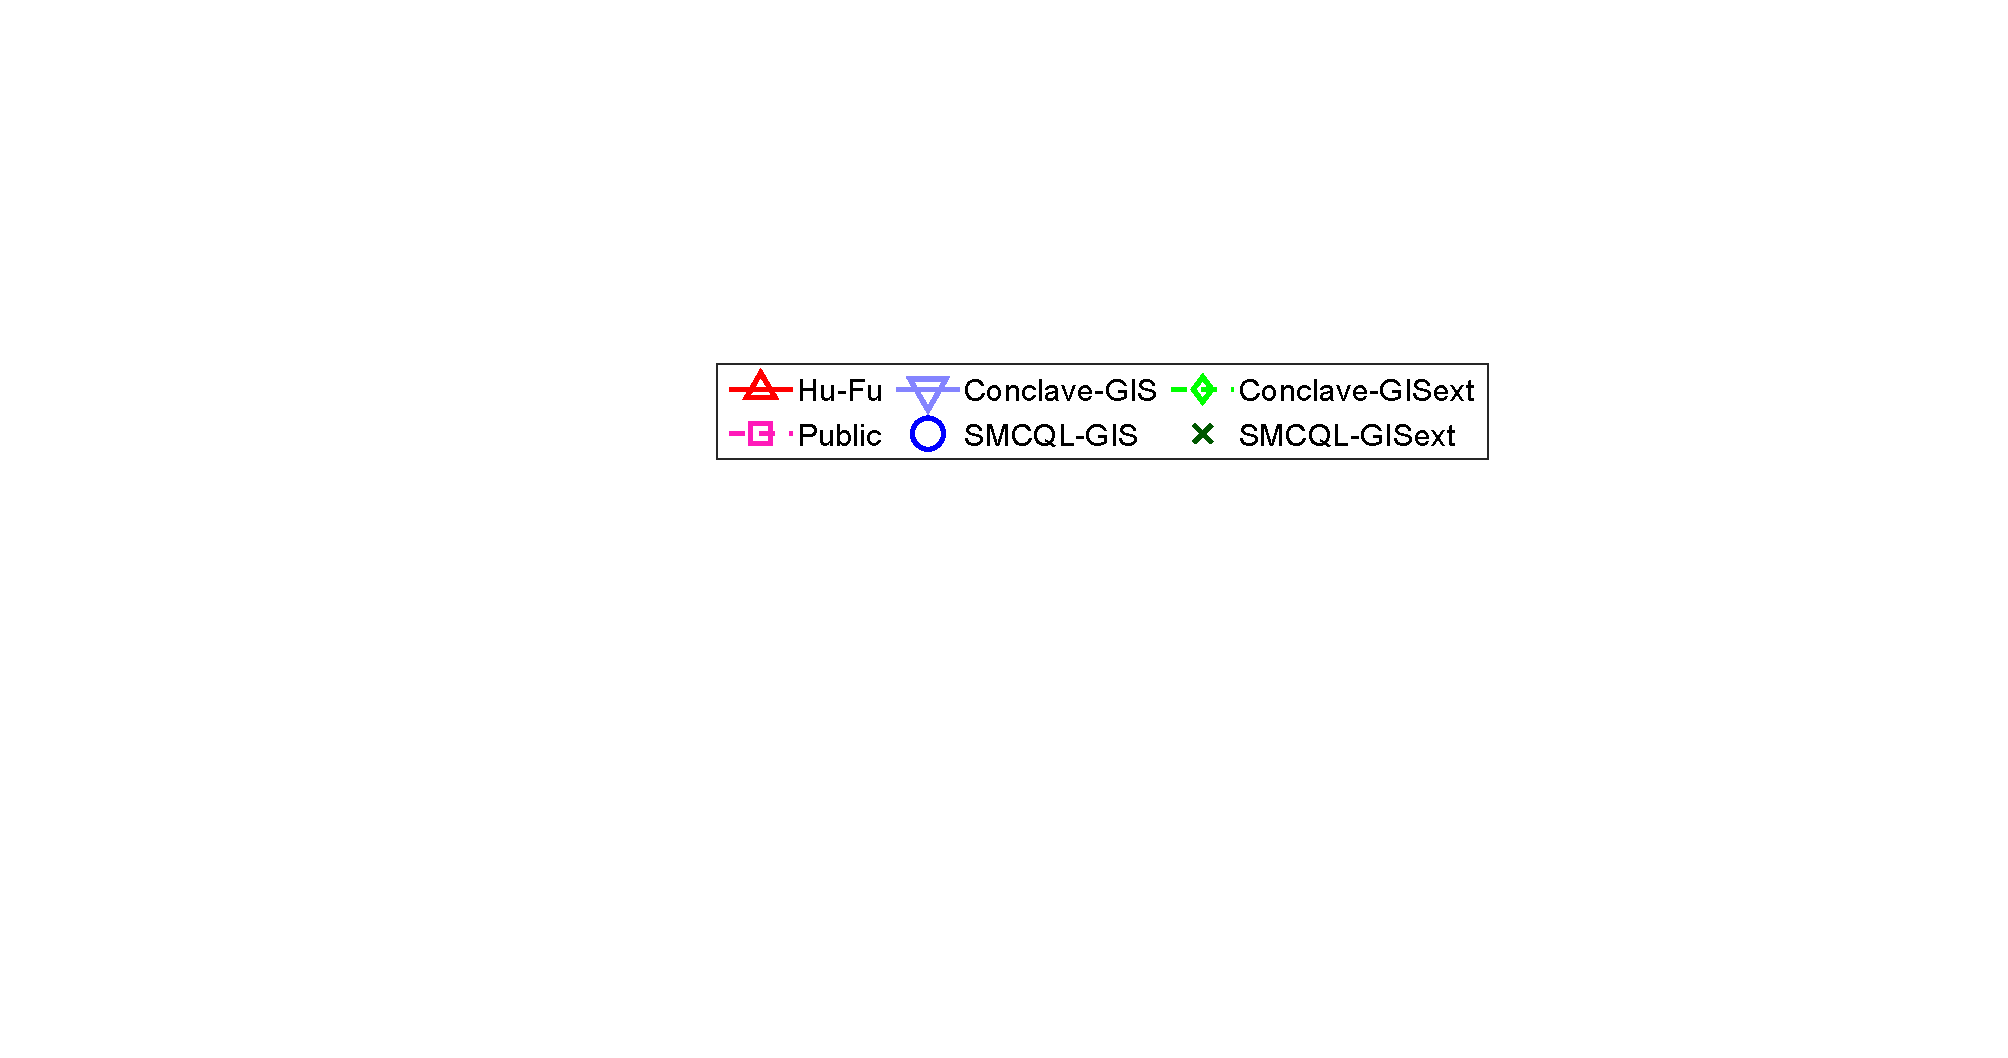
\includegraphics[width=\textwidth]{legend.pdf}
    \end{subfigure}
    \begin{subfigure}{0.48\textwidth}
        \centering
        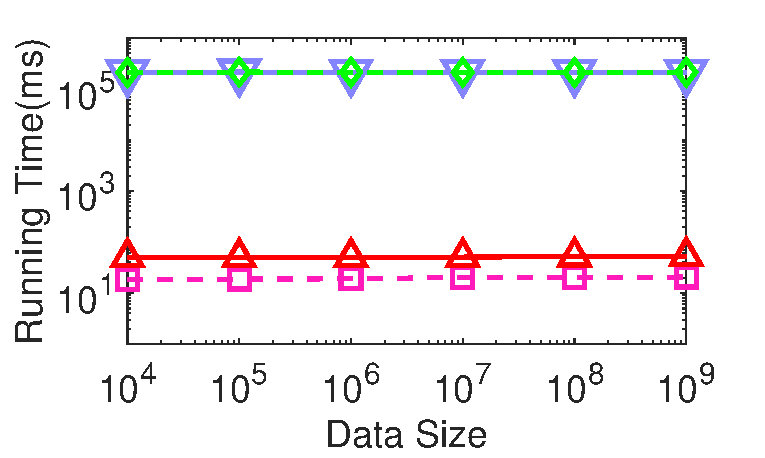
\includegraphics[width=0.48\linewidth]{knn_datasize_time.pdf}
        \includegraphics[width=0.48\linewidth]{knn_datasize_cost.pdf}
        \caption{Scalability test of federated kNN query}
        \label{fig:knn-eff-size-n}
    \end{subfigure}
    \begin{subfigure}{0.48\textwidth}
        \centering
        \includegraphics[width=0.48\linewidth]{knnjoin_datasize_time.pdf}
        \includegraphics[width=0.48\linewidth]{knnjoin_datasize_cost.pdf}
        \caption{Scalability test of federated kNN join}
        \label{fig:knn-j-eff-size-n}
    \end{subfigure}
    \begin{subfigure}{0.48\textwidth}
        \centering
        \includegraphics[width=0.48\linewidth]{rangecount_datasize_time.pdf}
        \includegraphics[width=0.48\linewidth]{rangecount_datasize_cost.pdf}
        \caption{Scalability test of federated range counting}
        \label{fig:count-eff-size-n}
    \end{subfigure}
    \begin{subfigure}{0.48\textwidth}
        \centering
        \includegraphics[width=0.48\linewidth]{rangequery_datasize_time.pdf}
        \includegraphics[width=0.48\linewidth]{rangequery_datasize_cost.pdf}
        \caption{Scalability test of federated range query}
        \label{fig:range-eff-size-n}
    \end{subfigure}
	\begin{subfigure}{0.48\textwidth}
        \centering
        \includegraphics[width=0.48\linewidth]{dj_datasize_time.pdf}
        \includegraphics[width=0.48\linewidth]{dj_datasize_cost.pdf}
        \caption{Scalability test of federated distance join}
        \label{fig:distjoin-eff-size-n}
    \end{subfigure}
    \caption{Scalability test on asymmetric queries.}
    \label{fig:exp-scala}
\end{figure}

\subsubsection{Scalability Test on Asymmetric Queries}
\label{subsec:exp-asymm-scalability}

\fakeparagraph{Parameter Setting}
In the following, we scale the total number of spatial objects from $10^4$ to $10^9$ over OSM dataset to assess the scalability of \sysname.
Other parameters are set to the default values as in \secref{subsec:exp-cmp}.
For example, the number of silos is $6$, $k=16$ for federated kNN query and kNN join, and the query area for federated range query, range counting and distance join is $0.001\%$.
Since \smcql and \smcqlext only support two silos, they are excluded in the scalability test.
The running time and communication cost on all five spatial queries are shown in \figref{fig:exp-scala}.

\fakeparagraph{Result and Analysis}
For a fixed data size, we observe that \sysname is notably more efficient than \conclave and \conclaveext on federated kNN query, kNN join and range counting (see \figref{fig:knn-eff-size-n}-\ref{fig:count-eff-size-n}).
For federated range query and distance join, \conclave behaves the same as Public due to the honest broker, while \sysname achieves the same efficiency as \conclaveext, which requires no honest broker.

We are more interested in the efficiency with the increase of data size.
We observe that the efficiency of federated kNN query, kNN join and range counting is insensitive to the increase of the data size.
This is because the increase of data size mainly affects the time cost of plaintext primitives, which only accounts for a small portion (due to efficient indexes in each silo) in the running time.
In contrast, the running time and communication cost of federated range query and distance join notably increase with the increase of the data size because more spatial objects are retrieved in each silo, which leads to a higher cost for both plaintext range query and secure set union.

\fakeparagraph{Takeaways} 
\sysname trivially scales with data size for federated kNN query, kNN join and range counting, because these queries are relatively insensitive to data size.
Both metrics of \sysname increase with the data size for federated range query and distance join, yet \sysname is still reasonably efficient for them on large-scale data.
For example, in \sysname, an asymmetric federated range query takes 250 ms running time and 2.6 MB communication cost on the data size of $10^9$.

\subsubsection{Scalability Test on Symmetric Queries}
\label{subsec:exp-symm-scalability}

\fakeparagraph{Parameter Setting}
As for symmetric queries, we evaluate the scalability of \sysname by scaling the OSM dataset, gradually increasing the total number of spatial objects from $10^4$ to $10^8$.
The baseline selection here is identical to that in \secref{subsec:exp-symmetric}.
Although we omit the results of spatial joins,
the scalability of the federated distance join and kNN join can be inferred from the scalability of the federated range query and kNN query, as demonstrated in the previous experiments in \secref{subsec:exp-cmp} and \secref{subsec:exp-symmetric}.

\fakeparagraph{Result and Analysis}
As shown in \figref{fig:sym-exp-scala}, for any data size, \sysname significantly outperforms \conclave and \EDBT in both running time and communication overhead for all the tested queries. 
For example, in \figref{fig:sca-knn-eff-size-n}, \sysname is at least 54.8$\times$ and 1375.7$\times$ faster than \conclave and \EDBT, respectively. 
Neither \conclave nor \EDBT can efficiently process these queries over large-scale datasets (\eg when the data size is over $10^6$).
After running for more than 6 hours, neither of them have terminated, so we are unable to obtain their full results.
Moreover, when processing symmetric federated range queries, both \conclave and \EDBT take at least 2 orders of magnitude higher communication cost than \sysname.

By contrast, \ICDE is slightly faster than \sysname (no more than 2.8$\times$) and has lower communication overhead in \figref{fig:sca-rangquery-eff-size-n}.
However, since \ICDE may violate the data privacy during the query processing and can only obtain approximate results,
the performance gap is acceptable.
For instance, the recall of \ICDE can be lower than 80\%, and such a low recall may lead to an unsatisfying service experience in our motivation scenarios like contact tracing, where accurate results are crucial.

\begin{figure}[t]
    \centering
    \begin{subfigure}{0.48\textwidth}
        \centering
        \includegraphics[width=0.48\linewidth]{osm_knn_size_time.pdf}
        \includegraphics[width=0.48\linewidth]{osm_knn_size_comm.pdf}
        \caption{Scalability test of federated kNN query}
        \label{fig:sca-knn-eff-size-n}
    \end{subfigure}
    \begin{subfigure}{0.48\textwidth}
        \centering
        \includegraphics[width=0.48\linewidth]{osm_rangequery_size_time.pdf}
        \includegraphics[width=0.48\linewidth]{osm_rangequery_size_comm.pdf}
        \caption{Scalability test of federated range query}
        \label{fig:sca-rangquery-eff-size-n}
    \end{subfigure}
    \begin{subfigure}{0.48\textwidth}
        \centering
        \includegraphics[width=0.48\linewidth]{osm_rangecount_size_time.pdf}
        \includegraphics[width=0.48\linewidth]{osm_rangecount_size_comm.pdf}
        \caption{Scalability test of federated range counting}
        \label{fig:sca-rangecount-eff-size-n}
    \end{subfigure}
    \caption{Scalability test on symmetric queries.}
    \label{fig:sym-exp-scala}
\end{figure}

\fakeparagraph{Takeaways} 
Unlike the scalability tests for asymmetric queries, the efficiency of symmetric federated range query, range counting, and kNN query is highly sensitive to the data size.
Specifically, when processing \textit{asymmetric queries}, all compared solutions leverage plaintext operators to filter most of the data objects.
For example, a plaintext range query can ensure no false positive candidate for asymmetric federated range queries, while a plaintext kNN query results in only $k$ false positive candidates for asymmetric federated kNN queries.
Consequently, the number of false positive candidates is (almost) independent of data size.

However, when processing \textit{symmetric queries} that require additional protections for the query location, although plaintext operators are still used to reduce the candidate size, no solution can ensure a constant number of false positive candidates.
Even in our \sysname, the number of candidate objects awaiting secure verification after filtering by plaintext operators is proportional to the data size.
This contributes to the increased time and communication overhead required to process symmetric queries compared to asymmetric ones.

\subsection{Experiments on Heterogeneous Data Silos}
\label{subsec:exp-hete}
This experiment aims to demonstrate the feasibility of \sysname on heterogeneous spatial databases.
Specifically, we use $6$ different databases for each silo on the BJ dataset: PostGIS~\cite{postgis}, MySQL~\cite{mysql}, SpatiaLite~\cite{spatialite}, Simba~\cite{sigmod16simba}, GeoMesa~\cite{ds15geomesa}, and SpatialHadoop~\cite{icde15spatialhadoop}.
Other parameters are set as the default values as in \secref{subsec:exp-cmp}.

\begin{figure}[t]
    \centering
    \includegraphics[width=0.46\textwidth]{database_compare.pdf}
    \caption{Running time breakdown.}
    \label{fig:database-cmp}
\end{figure}

\figref{fig:database-cmp} plots the running time breakdown \ie plaintext vs. secure primitives for radius-unknown (\ie asymmetric federated kNN query) and radius-known (\ie asymmetric federated range counting) queries.
We make the following observations.
\begin{itemize}
    \item 
    Given homogeneous underlying spatial databases (\ie PostGIS), our \sysname significantly reduces the running time of secure primitives \eg $3,935.4\times$ compared with \conclave for federated kNN query.
    Such acceleration in secure primitives is the primary contributor to \sysname's gain in running time.
    
    \item
    Heterogeneous underlying spatial databases affect the running time.
    Specifically, the running time of plaintext primitives is limited by the slowest spatial database, which may increase the overall query processing time.
    In this experiment, the running time of plaintext primitives notably increases from $4$ ms to $579$ ms when replacing PostGIS with heterogeneous databases (where SpatiaLite and MySQL are the slowest). It takes even longer time than the secure primitives in \sysname.
    The running time of secure primitives also marginally increases, due to idle waiting for the local results from the slowest silo.
\end{itemize}

For other symmetric federated spatial queries (\ie range query, distance join, and kNN join), please refer to \appref{app:exp-2} for their detailed results.

\fakeparagraph{Takeaways} 
\sysname functions with data silos running heterogeneous databases.
Although \sysname dramatically speeds up the secure primitives in a federated spatial query, the efficiency of plaintext primitives in each silo's databases may affect the overall running time.
Particularly, the time cost of plaintext primitives can be limited by the slowest database in the federation.
To unleash the full potential of \sysname, fast spatial databases in each silo are recommended.

\section{Related Work}
\label{sec:related}

Distributed spatial database systems are popular solutions to query processing on big spatial data.
These systems improve query processing via data partition and indexing techniques (\eg R-tree \cite{DBLP:series/synthesis/2011Mamoulis}) in Hadoop (\eg SpatialHadoop~\cite{icde15spatialhadoop}) or Spark (\eg Simba~\cite{sigmod16simba}).
However, the data partition techniques are inapplicable in a data federation since the entire data is held by the autonomous data silos.
Moreover, security is not the major concern in these systems.

Past studies of secure spatial query processing mainly focus on encrypted databases \cite{hacigumucs2002executing}, where data is encrypted and stored in a third-party platform (\eg a cloud platform) to process queries securely.
For example, existing work \cite{DBLP:conf/sigmod/WongCKM09,DBLP:conf/icde/0002LX13,DBLP:conf/icde/ElmehdwiSJ14,DBLP:conf/edbt/KesarwaniKNPSMM18} study the secure kNN query on encrypted databases and prior studies \cite{DBLP:conf/icde/WangR13,DBLP:conf/icde/WuLLYYW19,DBLP:conf/icde/SahinAAAP18,DBLP:conf/edbt/TranAdA19} focus on securely processing range queries.
In these studies, a data owner outsources its data and hence the sensitive data is encrypted before being uploaded to a third party.
Intuitively, homomorphic encryption techniques (\eg Paillier and SEAL~\cite{DBLP:journals/csur/AcarAUC18}) are used to guarantee security. 
Different from this setting, in a data federation, data silos autonomously manage their own data and hence do not need to encrypt their own data and upload it to a third party.
Besides, our experiments demonstrate that extending these solutions \cite{DBLP:conf/icde/SahinAAAP18,DBLP:conf/edbt/KesarwaniKNPSMM18} to the scenario of the data federation can be either insecure or inefficient.

Rather than the general distributed databases or outsourced databases, our work is more aligned with the problem settings of federated databases and data federation, where the entire dataset is held in multiple autonomous databases.
Early research on federated databases focused on finding solutions to access data in autonomous databases \cite{DBLP:books/sp/OzsuV20}, while recent studies on federated databases support diverse data types, \eg on federated graph databases \cite{DBLP:conf/www/VuAEJ19}. 
Note that the autonomous database here means that data can be only managed by its held silo. 

Data federation is an emerging concept developed from federated databases. 
It shares a similar architecture with federated databases.
Yet, the \textit{major difference} is that a data federation imposes certain secure requirements during query processing, while a federated database does not.
For example, SMCQL~\cite{vldb17smcql} is probably the first secure query processing solution over a data federation and Conclave~\cite{eurosys19conclave} is the state-of-the-art solution.
More recent studies explored efficient solutions to join queries \cite{DBLP:conf/sigmod/Wang021, 10463171, DBLP:conf/icde/HanZFLL22} in a data federation.
All these studies adopt SMC techniques to achieve secure query processing for \textit{relational} data with \textit{exact} results.

Exact federated queries have been explored for various data types. 
Our preliminary work \cite{DBLP:journals/pvldb/TongPZSXZZCXXL22} and its accompanying demonstration system \cite{DBLP:journals/pvldb/PanTXZDZSZCXXL22} focus on exact federated queries over spatial data federation.
Zhang \etal \cite{DBLP:journals/pacmmod/ZhangWXPX24} propose an efficient method that leverages the Intel SGX to securely perform similarity searches over a data federation under metric spaces.
For example, the metric distance can be the graph edit distance for graph data or the edit distance for sequence data. 

Existing studies also investigate \textit{approximate} query processing over a data federation.
SAQE~\cite{DBLP:journals/pvldb/BaterP0WR20}, Crypt$\epsilon$ \cite{DBLP:conf/sigmod/ChowdhuryW0MJ20}, and Shrinkwrap~\cite{DBLP:journals/pvldb/BaterHEMR18} use differential privacy to trade off between accuracy and efficiency in processing relational queries.
Others study approximate kNN queries \cite{DBLP:conf/dasfaa/ZhangTSZXCZXLZ23} and range counting \cite{DBLP:conf/dasfaa/LiZC23,tkde21shi} over a spatial data federation.
In contrast, we focus on \textit{exact} query processing, since accurate results can be crucial for spatial applications like contact tracing~\cite{2020quantifying}. 

In short, our work is inspired by the emerging trend of secure query processing over a data federation, yet focuses on spatial queries with exact results. 
Our \sysname significantly improves the efficiency of federated spatial queries over the extensions of SMCQL~\cite{vldb17smcql} and Conclave~\cite{eurosys19conclave}, the state-of-the-arts for relational data.
Moreover, unlike most existing studies that solely focus on protecting data privacy under this emerging scenario, \sysname also considers the application need for preserving the query privacy.
For example, in applications like contact tracing, spatial queries often contain sensitive location data of patients, thereby necessitating the protection on the query privacy.

\section{Conclusion}
\label{sec:conclusion}
In this paper, we propose the first system \sysname for efficient and secure spatial queries over a data federation.
Existing solutions are inefficient to process such queries due to excessive secure distance operations and the usage of general-purpose secure multi-party computation (SMC) libraries for implementing secure operators.
To overcome the inefficiency, we design a novel query rewriter to decompose the spatial queries into as many plaintext operators and as few secure operators as possible.
In particular, our secure operators have dedicated implementations faster than general-purpose SMC libraries.
Moreover, \sysname supports heterogeneous spatial databases (\eg PostGIS, Simba, GeoMesa, and SpatialHadoop), as well as query input in native SQL.
Finally, extensive experiments show that \sysname is up to 4 orders of magnitude faster and takes 5 orders of magnitude lower communication cost
than the state-of-the-arts.
In the future study, we plan to support more spatial queries, \eg spatial keyword search.

% \begin{acknowledgements}
%     This work is partially supported by National Key Research and Development Program of China under Grant No. 2023YFF0725103, 
%     National Science Foundation of China (NSFC) (Grant Nos. 62425202, U21A20516, 62336003, 62076017) and Beijing Natural Science Foundation (Z230001), 
%     Beijing Advanced Innovation Center for Future Blockchain and Privacy Computing (GJJ-23-004), The Fundamental Research Funds for the Central Universities No. JK2024-03, 
%     the Basic Research Funding in Beihang University No.YWF-22-L-531, and Didi Collaborative Research Program NO2231122-00047.
%     Zimu Zhou’s research is supported by Chow Sang Sang Group Research Fund No. 9229139.
%     Yuxiang Zeng is the corresponding author.
% \end{acknowledgements}

\bibliographystyle{spbasic.bst}     
\bibliography{fedsys}

\clearpage
\appendix
\section{Application Scenarios of Query Privacy}
\label{app:query-privacy-app}

Due to legal regulations (\eg GDPR~\cite{GDPR}), protecting \textit{data privacy} is now common in real-life scenarios, especially when spatial location implies the travel patterns or trajectories of a user. 
\textit{Query privacy} is equally important has numerous application scenarios. Here are some detailed examples:

\begin{enumerate}
    \item \textbf{Navigation}: Apps like Google Maps \cite{googlemaps} and Waze \cite{waze} frequently query user locations to provide directions and traffic updates. Revealing exact locations can expose sensitive information about users' daily routines and personal lives.
    
    \item \textbf{Social Networking}: Platforms like Facebook \cite{facebook} and Instagram \cite{instagram} allow users to check in at various locations. Protecting the privacy of these check-ins is crucial to prevent stalking and harassment.
    
    \item \textbf{Location-based Advertising}: This service targets users based on their current or recent locations. Protecting user privacy ensures that advertisers do not have access to sensitive location data, which could be misused for targeted marketing.

    \item \textbf{POI Search}: Applications like Yelp \cite{yelp} and TripAdvisor \cite{tripadvisor} allow users to search for nearby points of interest like restaurants, cafes, or hotels. Ensuring the privacy of sensitive location data will prevent potential tracking and profiling of users’ movement patterns by the platform.
\end{enumerate} 

Please refer to \cite{DBLP:reference/sp/2018mdp,DBLP:conf/esorics/2009-5599} for more application scenarios of query privacy.

\section{Security Analysis}
\label{app:secure}
The security analysis of our query rewriter is based on the composition lemma in \cite{goldreich2009foundations} (see its Sec. 7.3.1).
The lemma states that given a secure protocol $\pi^{g|f}$ that can securely compute $g$ based on a plaintext query $f$ and a secure protocol $\pi^f$ for operation $f$, the operation $g$ can be securely computed by executing protocol $\pi^{g|f}$ but substitutes every plaintext query $f$ with an execution of $\pi^f$.

We prove the security of query rewriter for asymmetric federated queries (\appref{app:secure-asym}) and symmetric federated queries (\appref{app:secure-symm}) separately.
Finally, we present a case study on attacking asymmetric federated range counting in \appref{app:secure-case}.

\subsection{Security Analysis of Asymmetric Federated Queries}\label{app:secure-asym}

In the following, we conduct a thorough analysis of the security of asymmetric federated queries in \sysname, categorizing them into two distinct kinds: \textit{radius-known queries} and \textit{radius-unknown queries}. 

\begin{itemize}
    \item \textbf{Security of Radius-Known Queries.} Federated range query, range counting and distance join belong to \textit{radius-known queries}.
    For \textit{federated range query} and \textit{distance join}, the secure protocol $\pi^{g|f}$ is the secure set union (\defref{def:ssun}) based on the query results of one or multiple plaintext range queries over the federation.
    The protocol $\pi^f$ corresponds to the plaintext range query (\defref{def:prq}).
    The protocol $\pi^f$ is secure, since the plaintext range query only occurs in each silo, which will not leak any information to other silos.
    From the composition lemma, federated range query and distance join are secure against semi-honest adversaries.
    Federated range counting is also secure based on a similar proof (\ie replacing $\pi^{g|f}$ with the secure summation in \defref{def:ssum} and $\pi^f$ with the plaintext range counting in \defref{def:prq}).
    
    \item \textbf{Security of Radius-Unknown Queries.} The federated kNN query and kNN join belong to \textit{radius-unknown queries}.
    For federated kNN query (\algref{alg:knn}), let protocol $\pi^f$ be the secure count comparison between $k$ and the local counts.
    The security of $\pi^f$ can be proved in the same way as before.
    Denote protocol $\pi^{g|f}$ as \algref{alg:knn} based on the plaintext count comparison query.
    We then show protocol $\pi^{g|f}$ is also secure.
    Assuming semi-honest adversaries, each silo can simulate its view of the execution of the protocol.
    Specifically, knowing the range $[l, u]$ used at the beginning of a round, each silo can compute $\thres$ used in that round.
    If $\thres$ is the same as the final radius, it concludes that the protocol must have ended in this round.
    Otherwise, it simply updates the range to that side of $\thres$ which contains the final radius.
    Along with the knowledge of the initial range, this shows that each silo can simulate the execution of the protocol, which means the protocol $\pi^{g|f}$ is secure.
    Thus, our \algref{alg:knn} is secure against semi-honest adversaries based on the composition lemma.
    The security of federated kNN join can be proved similarly.
\end{itemize}

\subsection{Security Analysis of Symmetric Federated Queries}\label{app:secure-symm}

Similar to the previous security analysis, we analyze the security of symmetric federated queries in \sysname from two categories: \textit{radius-known queries} and \textit{radius-unknown queries}. 

\begin{itemize}
    \item \textbf{Security of Radius-Known Queries.} 
    For \textit{federated range query}, the secure protocol $\pi^{g|f}$ employs the secure distance comparison (\defref{def:sdcmp}), which relies on the fully homomorphic encryption (FHE) scheme (\ie the BGV scheme \cite{DBLP:journals/csur/AcarAUC18}), and the secure set union (\defref{def:ssun}).
    The protocol $\pi^f$ corresponds to the plaintext range query (\defref{def:prq}).
    It is secure because the plaintext range query is executed within each silo individually, thereby preventing any information leakage to other silos.
    According to the composition lemma, the query rewriter for symmetric federated range queries ensures data privacy.
    Regarding the additional privacy requirement of query privacy, the secure protocol, secure location perturbation (\defref{def:sdp}), is based on the BPL mechanism in \cite{DBLP:journals/corr/abs-2312-12012}.
    This mechanism has been proven to satisfy $(\epsilon,\delta)$-Geo-Indistinguishability (Geo-I) \cite{DBLP:conf/ccs/AndresBCP13}, a widely-adopted privacy notion for preserving location privacy.
    Thus, the query privacy is due to the protection of query location with secure location perturbation.
    As for \textit{federated distance join}, the data privacy and query privacy can be guaranteed, since a federated distance join is decomposed into a series of federated range queries, and the security of each federated range query has been proven.
    The security of \textit{federated range counting} shares similarities with that of federated range query, primarily due to their near-identical decomposition plans (see \tabref{tab:sym-rewriter}).
    However, a key difference lies in the nature of their query answers. 
    While federated range query requires a secure set union to collect spatial objects falling within the specified range, federated range counting simply returns an integer count as its output. 
    This distinction underscores the minimal exposure of information in federated range counting, further reinforcing its security.
    
    \item \textbf{Security of Radius-Unknown Queries.} 
    To prove the security of radius-unknown queries, we only need to show the security of federated kNN query,
    since a federated kNN join is decomposed into multiple independent federated kNN queries by \sysname.
    Similar to the decomposition plan for asymmetric federated kNN query, the query rewriter for symmetric federated kNN query also utilizes a binary-search procedure.
    The key difference is that the initial upper bound is determined by plaintext kNN queries and secure location perturbation.
    Thus, for this step, the secure protocol $\pi^{g|f}$ is due to the privacy guarantee of $(\epsilon,\delta)$-Geo-Indistinguishability (Geo-I) \cite{DBLP:conf/ccs/AndresBCP13}.
    The security analysis for the other steps is similar to that for asymmetric radius-unknown queries.
\end{itemize}

\subsection{Case Study on Semi-Honest Attack}\label{app:secure-case}

\begin{table}[t]
    \centering
    \caption{A case study on hacking (asymmetric) federated range counting in \sysname.}
    \begin{small}
    \begin{tabular}{ccc}
		\toprule
		\makecell[c]{Colluded\\silos} & \makecell[c]{Attack\\success rate}  & \makecell[c]{Running\\time}  \\
		\midrule
		1             & $0$         & No result for 2 months    \\
		2             & $0$         & No result for 2 months    \\
		3             & $0$         & No result for 2 months    \\
% 		4             & $2.56\%$    & 173.23 s       \\
		\bottomrule
    \end{tabular}
    \end{small}
    \label{tab:attack}
\end{table}

\fakeparagraph{Case Study}
We have also conducted a case study to show how \sysname defenses against the semi-honest adversaries when processing asymmetric federated range counting.

\begin{itemize}
    \item \textbf{Experimental Setup.} The case study is based on the BJ dataset with 6 silos (\ie our default setting) and we vary the number $m$  of colluded adversaries (\ie silos) from 1 to 3. Then, when processing asymmetric federated range counting, the attack will occur at the only secure operator (\ie secure summation \cite{DBLP:journals/dke/EmekciSAA07}). To attack the secure summation, we use the method introduced in ~\cite{DBLP:journals/dke/EmekciSAA07}. In general, a secure operator successfully defenses against the attack, if adversaries cannot get any feasible result after a long time (\eg two months in our experiment). Furthermore, the other experiment parameters are the same as those in \secref{subsec:exp-cmp}.
    
    \item \textbf{Experimental Result.} 
    As shown in \tabref{tab:attack}, even when 50\% of the silos collude, they cannot infer any feasible result even after two months' cracking.
    Note that it is commonly assumed in existing work that the portion of colluded adversaries is less than 50\%.
    Based on the computational security \cite{DBLP:reference/dbsec/2008,goldreich2009foundations,DBLP:conf/ccs/Bayatbabolghani18}, this result proves \sysname is hard to attack.
\end{itemize}

\section{Handling Ties in Symmetric Federated kNN Query}
\label{app:knn-tie}

We provide a solution for handling ties in symmetric federated kNN query and conduct an experimental comparison.
\textbf{Main Idea.} To break our assumption and handle the special case of ties, we need to address two question: (1) how to identify such cases and (2) how to retrieve exactly $k$ nearest neighbors, using the following ideas:
\begin{enumerate}[(1)]
    \item \textbf{Identify such cases}.
    For any searching radius $r$ during the binary-search, whenever the total number of spatial objects closer to the query object $q$ than $r$ is equal to $k$ (\ie the result of secure count comparison is $sign = 0$), we can find exactly $k$ nearest neighbors (\ie there are no other objects whose distances to $q$ are also the $k$th nearest distances).
    When the binary-search terminates and $sign$ is always non-zero, we will encounter the mentioned case (we call it ``ties'' for brevity).
    
    \item \textbf{Retrieve exactly $k$ nearest neighbors}.
    Under this case, we will obtain the final lower bound $l$ and upper bound $u$ of the searching radius for $k$th nearest neighbor.
    Since the binary-search has been terminated, we can derive that $u-l$ must be smaller than the distance precision $\epsilon_0$.
    Now, we \textit{first} use the circular range $\text{circle}(q,l)$ to locate all spatial objects that are strictly inside the circle curve (\ie by a symmetric federated range query), and denote the total count as $k_l$.
    Notice that we can temporarily cache the partial answers in each data silo at this step.
    \textit{Next}, we only need to randomly pick $k-k_l$ spatial objects from those objects on the circle curves.
    To achieve this goal, we sequentially request such spatial objects from every data silo,
    and set a limitation on how many spatial objects are indeed required.
    \textit{Lastly}, a secure set union operator is used to collect the $k$ nearest neighbors, since the partial answer has been cached in each data silo.
\end{enumerate}

\begin{figure}[t]
    \centering
    \includegraphics[width=0.45\textwidth]{apdx/example.pdf}
    \caption{Illustration of the special case of symmetric federated kNN query ($k=6$).}
    \label{fig:special-knn}
\end{figure}

\algref{alg:tie-knn} illustrates the detailed procedure of using the main idea to process the cases of ties.
Specifically, lines 3-9 represent the procedure of binary-search.
In line 10, when $sign$ equals 0 in some iteration of the binary search, we know the current searching radius $\thres$ is already enough to retrieve the exact $k$ nearest neighbors.
A symmetric federated range query can drive the query answer.
By contrast, in line 12, $sign$ has never become $0$, then we know we are facing the case of ties now.
To handle this case, line 14 computes how many data objects are strictly inside the circle curve, denoted by $k_l$.
Thus, we only need to pick $k-k_l$ from those tied objects on the circle curve.
To do so, lines 16-20 sequentially request certain objects from each data silo, and limit the number of retrieved object no larger than $remain$ (since we do not need more).
To avoid data objects are duplicate statistics, lines 14 and 17 will cache the (partial) answer locally at each silo.
Finally, line 20 collects the query answer from all data silos.

To ease of understanding, \expref{exp:special-knn} is used to further illustrate the main idea.

\begin{example}\label{exp:special-knn}
    \figref{fig:special-knn} illustrates an instance as you mentioned,
    where $k$ is 6 and the distance precision $\epsilon_0$ is set to 1.
    \Song{Suppose the final upper bound $u$ is 10, and the final lower bound $l$ is 9.5.}
    When using the upper bound $u$ of 10 as the radius, the number of points is 9, which exceeds $k$. 
    When using the lower bound $l$ of 9.5 as the radius, the number of points is 3, which is fewer than $k$. 
    Since the difference between the bounds, $u-l=0.5$, is less than the distance precision $\epsilon_0=1$, the binary search has been terminated and we can identify the case of ties.
    As shown in \figref{fig:special-knn}, this case introduces a challenge in handling boundary points to ensure that exactly $k$ spatial objects are retrieved as the $k$ nearest neighbors. 
   To address this issue, we use the following strategy to manage these boundary spatial objects. 
   
   \begin{enumerate}[(1)]
    \item
    % during the binary-search process, each silo caches the sets of all points corresponding to both the upper and lower bounds.
    We perform a symmetric federated range query with the query object $q$ (marked in red color in \figref{fig:special-knn}) and the circle radius $l = 9.5$.
    The query answer (\ie the three objects within the inner circle) will be cached individually within each data silo.
    Besides, these data silos collaboratively and securely compute the total count $k_l = 3$.
    
    % In this example, when querying with the upper bound, each silo caches 3 points, resulting in a total of 9 points, with the cache for each silo denoted as $Cand_i$. When querying with the lower bound, each silo caches 1 point, totaling 3 points, with the cache for each silo denoted as $Cand_i’$.
    
    \item Now, it is still 3 objects short of the required $k = 6$ objects.
    Moreover, we do not know the exact number of ties in each data silo, but need to retrieve exactly 3 additional objects from tied ones.
    Thus, we need to sequentially request up to 3 points from each silo. 
    Specifically, starting from data silo \#1, we perform a symmetric federated range query with the query object $q$ and the circle radius $u = 10$ in data silo \#1, and limit the number of (uncached) query answer to 3.
    Although there are three objects within the query area, one of them has already been cached before, meaning data silo \#1 can only provide two more answers as the $k$ nearest neighbors.
    After this step, we need to request one more point from data silos \#2 and \#3.
    Similarly, we perform a symmetric federated range query with the query object $q$ and the circle radius $u = 10$ in data silo \#2, and limit the number of (uncached) query answer as 1.
    In data silo \#2, three objects are within the query range, but one has been cached. 
    Then, data silo \#2 can randomly pick one from the two uncached points as the cached query answer. 
    At this point, we have obtained exactly $6$ spatial objects as the query answer, thus eliminating the need to request any additional (uncached) objects from data silo \#3.
    
    \item \textit{Lastly}, a secure set union is performed to collect all the cached spatial objects from the data silos, resulting in a final output that contains exactly the 6 nearest neighbors.
    \end{enumerate}
\end{example}


\setlength{\textfloatsep}{1ex}
\setlength{\floatsep}{1ex}
\begin{algorithm}[t]
	\caption{\small{Symmetric federated kNN query}}\label{alg:tie-knn}
	\KwIn{federation $F$, query object $q$, integer $k$}
	\KwOut{the (exact) query answer $ans$}
    $[l,u] \gets [0,U]$, where $U$ is the tight upper bound\;
    $q' \gets$ secure location perturbation $\geoi(q)$\;
    \While {$u - l \geq \epsilon_0$} {
        $\thres \leftarrow (l+u)/2$, $\mathcal{R} \gets \text{circle}(q, \thres)$\;
        $v_i \gets$ symmetric federated range counting in $F$ with circular range $\mathcal{R}$\; 
        $sign \gets$ secure count comparison $\scmp(\{v_i\}, k)$\;
        \textbf{if} $sign < 0$ \textbf{then} $l \leftarrow \thres$\;
        \textbf{else if} $sign > 0$ \textbf{then} $u \leftarrow \thres$\;
        \textbf{else} \textbf{break}\;
    }
    \If{$sign=0$}{
        % \ForEach(// perform in parallel){silo $F_i \in F$}{
        $ans \gets$ symmetric federated range query in $F$ with circular range $\text{circle}(q, \thres)$\; 
        % $ans$ $\gets$ secure set union $\ssun(S_1,\cdots,S_n)$\;
        % } 
        % $S_i \gets$ plaintext range query $\lrq(F_i, circle(q, \thres))$\;
    }
    \Else(// identify cases of ties \& retrieve exact kNN){
        $\mathcal{R}_l \gets \text{circle}(q, l)$,
        $\mathcal{R}_r \gets \text{circle}(q, r)$\;
        $k_{l} \gets$ symmetric federated range counting in $F$ with circular range $\mathcal{R}_l$ and cache all the spatial objects that are inside $\mathcal{R}_l$ locally at each silo\;
        \tcp{need to retrieve exactly $remain$ objects}
        $remain \gets k - k_{l}$\; 
        \ForEach(// perform in sequential){silo $F_i \in F$}{ 
            $k_r^i \gets$ symmetric federated range counting in $F_i$ with circular range $\mathcal{R}_r$ over uncached spatial objects at silo $F_i$, limit the query answer to $\le remain$, and cache the query answer locally at silo $F_i$\;
            $remain \gets remain - k_r^i$\;
            \lIf{$remain=0$}{\textbf{break}}
        }
        $ans$ $\gets$ secure set union $\ssun(S_1,\cdots,S_n)$ over all cached spatial objects within each data silo\;
    }
    \KwRet{$ans$}\;
\end{algorithm}
\afterpage{\global\setlength{\textfloatsep}{\oldtextfloatsep}}
\afterpage{\global\setlength{\floatsep}{\oldfloatsep}}

\textbf{Experimental Setup.}
Since we have not found such cases in our datasets (OSM and BJ), we generate a new synthetic dataset to conduct this experiment.
In the new synthetic dataset, there are six data silos and each data silo has 10,000 spatial objects.
We also fix $k$ as 16 (\ie our default setting) and vary the proportion (denoted by $\alpha$) of spatial objects strictly inside circle curve 25\%, 50\%, 75\%, and 100\%, respectively.
We also ensure that at least 16 spatial objects happen to be on the circle curve (\ie they are ``ties'').
In other words, when $\alpha=25\%$, $(1-25\%) \cdot k = 12$ spatial objects in the query answer are on the circle curve.
Similarly, when $\alpha=100\%$, no spatial object in the query answer is on the circle curve.

\begin{figure}[t]
    \centering
    \begin{subfigure}{0.48\textwidth}
        \centering
        \includegraphics[width=0.48\linewidth]{apdx/random_knn_corner_time.pdf}
        \includegraphics[width=0.48\linewidth]{apdx/random_knn_corner_comm.pdf}
    \end{subfigure}
    \caption{Performance of \Song{symmetric} federated kNN query in the synthetic dataset for handling ties.}
    \label{fig:random-knn-corner}
\end{figure}

\textbf{Experimental Result.}
\figref{fig:random-knn-corner} shows the experimental result. 
We can observe that our solution \sysname is still more efficient than the other baselines.
%The algorithm’s performance is not significantly affected by the proportion of spatial objects within the circle and remains relatively stable overall. 
Additionally, we also evaluate the total cost of our solution to the above two technical issues (\ie identifying the case of ties and retrieving exactly $k$ nearest neighbors).
The total time cost of these two steps remains within 400ms, and the communication cost stays under 400KB, accounting for 4.4\% of the total query time and 0.17\% of the total communication cost.

\section{Additional Experiments on Heterogeneous Data Silos}\label{app:exp-2}

\begin{figure}[t]
    \centering
    \includegraphics[width=0.48\textwidth]{apdx/database_compare_range.pdf}
    \caption{Running time breakdown.}
    \label{fig:database-cmp-range}
\end{figure}

\figref{fig:database-cmp-range} shows the results of asymmetric federated range query, distance join, and kNN join in the experiment of heterogeneous silos.
We can first observe that our \sysname can support all six spatial database systems, including PostGIS~\cite{postgis}, MySQL~\cite{mysql}, SpatiaLite~\cite{spatialite}, Simba~\cite{sigmod16simba}, GeoMesa~\cite{ds15geomesa}, and SpatialHadoop~\cite{icde15spatialhadoop}.
In addition, for all federated spatial queries in \figref{fig:database-cmp-range}, we observe the running time of \sysname becomes longer, compared with the results of homogeneous silos (\ie PostGIS in this test).
This is because the time cost of \sysname's plaintext primitives (\ie plaintext range query) increases due to the slowest spatial database system.
We can also observe that the experimental patterns of federated distance join and federated kNN join are similar to those of federated range query and federated kNN query.
This is because a federated distance/kNN join is decomposed into a series of federated range/kNN query.
Besides, we also recommend that all silos can use more efficient spatial database systems to further speed up the federated spatial queries.

This observation also holds for processing symmetric federated spatial queries, since the query processing procedure also involves plaintext primitives such as the plaintext range query and kNN query.

\begin{figure}[t]
    \centering
    \begin{subfigure}{0.45\textwidth}
        \centering
        \includegraphics[width=\textwidth]{apdx/legend.pdf}
    \end{subfigure}
    \begin{subfigure}{0.48\textwidth}
        \centering
        \includegraphics[width=0.48\linewidth]{apdx/knn_silo_time.pdf}
        \includegraphics[width=0.48\linewidth]{apdx/knn_silo_cost.pdf}
        \caption{Running time and communication cost of (asymmetric) federated kNN query}
        \label{fig:knn-eff-silo-n-ho}
    \end{subfigure}
    \begin{subfigure}{0.48\textwidth}
        \centering
        \includegraphics[width=0.48\linewidth]{apdx/knnjoin_silo_time.pdf}
        \includegraphics[width=0.48\linewidth]{apdx/knnjoin_silo_cost.pdf}
        \caption{Running time and communication cost of (asymmetric) federated kNN join}
        \label{fig:knn-j-eff-silo-n-ho}
    \end{subfigure}
    \begin{subfigure}{0.48\textwidth}
        \centering
        \includegraphics[width=0.48\linewidth]{apdx/rangecount_silo_time.pdf}
        \includegraphics[width=0.48\linewidth]{apdx/rangecount_silo_cost.pdf}
        \caption{Running time and communication cost of (asymmetric) federated range counting}
        \label{fig:count-eff-silo-n-ho}
    \end{subfigure}
     \begin{subfigure}{0.48\textwidth}
        \centering
        \includegraphics[width=0.48\linewidth]{apdx/rangequery_silo_time.pdf}
        \includegraphics[width=0.48\linewidth]{apdx/rangequery_silo_cost.pdf}
        \caption{Running time and communication cost of (asymmetric) federated range query}
        \label{fig:range-eff-silo-n-ho}
    \end{subfigure}
    \begin{subfigure}{0.48\textwidth}
        \centering
        \includegraphics[width=0.48\linewidth]{apdx/dj_silo_time.pdf}
        \includegraphics[width=0.48\linewidth]{apdx/dj_silo_cost.pdf}
        \caption{Running time and communication cost of (asymmetric) federated distance join}
    \end{subfigure}
    \caption{\sysname with an honest broker varying the silo number.}
    \label{fig:exp-honest-silo}
\end{figure}

\begin{figure}[t]
    \begin{subfigure}{0.45\textwidth}
        \centering
        \includegraphics[width=\textwidth]{apdx/legend.pdf}
    \end{subfigure}
     \begin{subfigure}{0.48\textwidth}
        \centering
        \includegraphics[width=0.48\linewidth]{apdx/knn_k_time.pdf}
        \includegraphics[width=0.48\linewidth]{apdx/knn_k_cost.pdf}
        \caption{Running time and communication cost of (asymmetric) federated kNN query}
        \label{fig:knn-eff-k-n-hon}
    \end{subfigure}  
     \begin{subfigure}{0.48\textwidth}
        \centering
        \includegraphics[width=0.48\linewidth]{apdx/knnjoin_k_time.pdf}
        \includegraphics[width=0.48\linewidth]{apdx/knnjoin_k_cost.pdf}
        \caption{Running time and communication cost of (asymmetric) federated kNN join}
        \label{fig:knn-j-eff-k-n-hon}
    \end{subfigure} 
     \begin{subfigure}{0.48\textwidth}
        \centering
        \includegraphics[width=0.48\linewidth]{apdx/rangecount_area_time.pdf}
        \includegraphics[width=0.48\linewidth]{apdx/rangecount_area_cost.pdf}
        \caption{Running time and communication cost of (asymmetric) federated range counting}
        \label{fig:count-eff-r-n-hon}
    \end{subfigure}
     \begin{subfigure}{0.48\textwidth}
        \centering
        \includegraphics[width=0.48\linewidth]{apdx/rangequery_area_time.pdf}
        \includegraphics[width=0.48\linewidth]{apdx/rangequery_area_cost.pdf}
        \caption{Running time and communication cost of (asymmetric) federated range query}
        \label{fig:range-eff-r-n-hon}
    \end{subfigure}
      \begin{subfigure}{0.48\textwidth}
        \centering
        \includegraphics[width=0.48\linewidth]{apdx/dj_area_time.pdf}
        \includegraphics[width=0.48\linewidth]{apdx/dj_area_cost.pdf}
        \caption{Running time and communication cost of (asymmetric) federated distance join}
        \label{fig:dj-eff-r-n-hon}
    \end{subfigure}  
    \caption{\sysname with an honest broker varying the query-specific parameter.}
    \label{fig:exp-honest-para}
\end{figure}

\section{Experiment on \sysname with an Honest Broker} \label{app:exp-hb}
In the following, we conduct an experiment to demonstrate the performance of \sysname with an honest broker (denoted by ``\sysname-HB'').

\fakeparagraph{Experimental Setup}
This experiment has tested all asymmetric federated spatial queries on the real-world dataset BJ. We compare \sysname-HB with \smcql/\conclave in query processing efficiency measured in running time and communication overhead. Besides, the other experiment settings are the same as those in \secref{subsec:exp-cmp}.

\fakeparagraph{Experimental Result}
\figref{fig:exp-honest-silo} and \figref{fig:exp-honest-para} present the experimental results of \sysname-HB and \smcql/\conclave in terms of running time and communication cost. First, We can observe that \sysname-HB performs the same as \smcql and \conclave on asymmetric federated range query and distance join. This is because all the compared algorithms (including ours) are simplified to Public due to the honest broker who collects the partial results (\ie sensitive data) of plaintext range query in each silo and is assumed to never reveal them to anyone else. Second, as for federated range counting, kNN query and kNN join, \sysname-HB still outperforms \smcql and \conclave with up to 4 orders of magnitudes faster in running time and 5 orders of magnitudes lower in communication cost. This is because our query writer is more effective to process queries on large-scale spatial data.

\fakeparagraph{Summary}
The experimental results demonstrate that compared to \smcql and \conclave, \sysname-HB exhibits similar efficiency in performing asymmetric federated range queries and distance joins. Additionally, \sysname-HB achieves better efficiency in asymmetric federated range counting, kNN queries, and kNN joins.
Although this experiment primarily focuses on asymmetric federated spatial queries, the observed patterns also apply to symmetric federated spatial queries. 
Specifically, the efficiency of symmetric federated range queries, distance joins, kNN queries, and kNN joins can be improved when an honest broker is present and a secure set union can be avoided.
However, in contrast to these operations, symmetric federated range counting is not affected by the presence of an honest broker, as it does not involve a secure set union operator in its decomposition plan (as shown in \tabref{tab:sym-rewriter}).

\section{Experiment on Geographically Partitioned Dataset} \label{app:exp-geo}
To explore the performance of \sysname in the dataset where each silo corresponds to a single country, we have conducted an experiment on a new synthetic dataset (denoted by ``\textit{OSM country}'').

\begin{table}[t]
    \centering
    \caption{Percentage of data of each country in \textit{OSM country}.}
    \begin{tabular}{cc}
		\toprule
		Country & Percentage of data  \\
		\midrule
		China             & $21.7\%$        \\
		India             & $29.8\%$        \\
		Japan             & $39.4\%$        \\
		Malaysia          & $4.2\%$         \\
		North Korea       & $1.2\%$         \\
		South Korea       & $3.7\%$         \\
		\bottomrule
    \end{tabular}
    \label{tab:country}
\end{table}

\fakeparagraph{Experimental Setup}
The \textit{OSM country} dataset consists of spatial points from six countries in OpenStreetMap~\cite{osm}. These countries include China, India, Japan, Malaysia, North Korea and South Korea, and each of them corresponds to a single data silo. As shown in \tabref{tab:country}, the volume of data in each silo follows the native data proportion of the corresponding country in OpenStreetMap. For example, the numbers of data points in China, India and Japan are much larger than those of Malaysia, North Korea and South Korea. Here, we vary the total number of all data points from $10^4$ to $10^9$. 
The query workloads are mainly asymmetric federated spatial queries.
Besides, the other experiment parameters are the same as those in \secref{subsec:exp-asymm-scalability}.

\fakeparagraph{Experimental Result}
The results of this experiment are shown in \figref{fig:exp-cty}. First, we can observe that in the \textit{OSM country} dataset, \sysname also shows a significant improvement in both running time and communication cost over \conclave and \conclaveext on federated kNN query, kNN join and range counting. For example, \sysname is at least 3 orders of magnitude faster than \conclave and \conclaveext in federated kNN query and kNN join, and costs 5 orders of magnitude lower network communication. Second, \sysname achieves the same efficiency as \conclaveext on federated range query and distance join. Overall, the ranking of the compared solutions in terms of either running time or communication cost is consistent with the ranking in \secref{subsec:exp-scalability}. Note that we exclude \conclaveext from the results of federated range counting as shown in \figref{fig:count-eff-size-n-cty}, because this query does not need the secure set union to protect data ownership in this query.

\begin{figure}[t]
    \begin{subfigure}{0.45\textwidth}
        \centering
        \includegraphics[width=\textwidth]{apdx/legend_scalability.pdf}
    \end{subfigure}
    \begin{subfigure}{0.48\textwidth}
        \centering
        \includegraphics[width=0.48\linewidth]{apdx/knn_datasize_time_revision.pdf}
        \includegraphics[width=0.48\linewidth]{apdx/knn_datasize_cost_revision.pdf}
        \caption{Running time and communication cost of (asymmetric) federated kNN query}
        \label{fig:knn-eff-size-n-cty}
    \end{subfigure}  
    \begin{subfigure}{0.48\textwidth}
        \centering
        \includegraphics[width=0.48\linewidth]{apdx/knnjoin_datasize_time_revision.pdf}
        \includegraphics[width=0.48\linewidth]{apdx/knnjoin_datasize_cost_revision.pdf}
        \caption{Running time and communication cost of (asymmetric) federated kNN join}
        \label{fig:knn-j-eff-size-n-cty}
    \end{subfigure}  
    \begin{subfigure}{0.48\textwidth}
        \centering
        \includegraphics[width=0.48\linewidth]{apdx/rangecount_datasize_time_revision.pdf}
        \includegraphics[width=0.48\linewidth]{apdx/rangecount_datasize_cost_revision.pdf}
        \caption{Running time and communication cost of (asymmetric) federated range counting}
        \label{fig:count-eff-size-n-cty}
    \end{subfigure}      
     \begin{subfigure}{0.48\textwidth}
        \centering
        \includegraphics[width=0.48\linewidth]{apdx/rangequery_datasize_time_revision.pdf}
        \includegraphics[width=0.48\linewidth]{apdx/rangequery_datasize_cost_revision.pdf}
        \caption{Running time and communication cost of (asymmetric) federated range query}
        \label{fig:range-eff-size-n-cty}
    \end{subfigure}      
     \begin{subfigure}{0.48\textwidth}
        \centering
        \includegraphics[width=0.48\linewidth]{apdx/dj_datasize_time_revision.pdf}
        \includegraphics[width=0.48\linewidth]{apdx/dj_datasize_cost_revision.pdf}
        \caption{Running time and communication cost of (asymmetric) federated distance join}
    \end{subfigure}   
    \caption{Scalability test on synthetic dataset partitioned by countries.}
    \label{fig:exp-cty}
\end{figure}

\fakeparagraph{Summary}
In this evaluation, \sysname outperforms \smcqlext and \conclaveext in terms of efficiency for asymmetric federated kNN queries, kNN join, and range counting. 
Meanwhile, \sysname performs comparably to \smcqlext and \conclaveext for asymmetric federated range queries and distance join.
Thus, we can conclude that the experiment conducted on the \textit{OSM country} dataset yields similar results to those observed in \secref{subsec:exp-asymm-scalability}. This similarity may stem from the fact that none of the existing methods have leveraged the data distribution in their query processing strategies.
Similarly, this new data partition is unlikely to alter the overall performance ranking of symmetric federated spatial queries. 

\section{Experiment on the Improvement by the Index in Each Data Silo}
\label{appendix:spatial-index}
To demonstrate that the federated spatial queries have already been accelerated by local indexes in \sysname, we have conducted a new experiment on the efficiency improvement caused by these local indexes (\ie R-trees in our default setting).

\fakeparagraph{Experimental Setup}
In this experiment, we test the running time of the plaintext spatial queries in \sysname (\ie plaintext range query, plaintext range counting and plaintext kNN query) on PostgreSQL with and without an R-tree. And the plaintext spatial queries are processed on the OSM dataset. Besides, we vary the data size from $10^4$ to $10^8$ and use the default setting of query area (0.001\%) and $k$ (16). The other experiment settings are the same as those in \secref{sec:experiment-setup}.

\fakeparagraph{Experimental Result}
As shown in \figref{fig:plaintext_query_index}, local indexes can improve the efficiency of plaintext spatial queries, especially when the data size is large. Specifically, the local index (R-tree) reduces the running time by up to $40\times$, $44\times$ and $2042\times$ when processing plaintext range query, range counting, and kNN query, respectively. Moreover, the plaintext spatial queries without local indexes cost even longer time than corresponding federated spatial queries in \sysname. For instance, the running time of processing one federated kNN query by \sysname takes 52 ms when the data size is $10^8$, which is even faster than that of the plaintext kNN query without the local index (2465 ms). Thus, the experimental result proves that we have used local indexes in \sysname to speed up the processing of the plaintext operators.

\begin{figure}[t]
    \centering
    \begin{subfigure}{0.48\textwidth}
        \centering
        \includegraphics[width=0.48\linewidth]{apdx/epsilon_knnquery_time.pdf}
        \includegraphics[width=0.48\linewidth]{apdx/epsilon_knnquery_comm.pdf}
        \caption{Runtime and communication cost of varying  $\epsilon$ in \sysname for processing symmetric federated kNN query}
        \label{fig:epsilon_knn}
    \end{subfigure}
    \begin{subfigure}{0.48\textwidth}
        \centering
        \includegraphics[width=0.48\linewidth]{apdx/epsilon_rangequery_time.pdf}
        \includegraphics[width=0.48\linewidth]{apdx/epsilon_rangequery_comm.pdf}
        \caption{Runtime and communication cost of varying $\epsilon$ in \sysname for processing symmetric federated range query}
        \label{fig:epsilon_rangequery}
    \end{subfigure}
    \caption{Impact of privacy budget $\epsilon$ in \sysname for processing symmetric federated kNN and range queries.}
    \label{fig:epsilon_eff}
\end{figure}

\begin{figure*}[t]
    \centering
    \begin{subfigure}{0.32\textwidth}
        \centering
        \includegraphics[width=\textwidth]{apdx/range_query_index.pdf}
        \caption{Plaintext range query}
        \label{fig:plain-range-query}
    \end{subfigure}
    ~
    \begin{subfigure}{0.32\textwidth}
        \centering
        \includegraphics[width=\textwidth]{apdx/range_count_index.pdf}
        \caption{Plaintext range counting}
        \label{fig:plain-range-counting}
    \end{subfigure}
    ~
    \begin{subfigure}{0.32\textwidth}
        \centering
        \includegraphics[width=\textwidth]{apdx/knn_index.pdf}
        \caption{Plaintext kNN query}
        \label{fig:plain-knn-query}
    \end{subfigure}
    ~
	\caption{Running time of plaintext spatial queries with/without R-tree.}
	\label{fig:plaintext_query_index}
\end{figure*}

\section{Impact of Additionally Protecting Query Privacy in Symmetric Queries on Time Cost}
\label{app:impact-query-privacy}

Symmetric queries generally exhibit slower performance compared to asymmetric queries.
The gap stems from the essential difference in the problem definition (\ie whether query privacy needs to be protected or not).
Consequently, accurately assessing the impact on time cost when incorporating query privacy protection is difficult.

However, we can roughly estimate the impact on time cost in two ways: 
\begin{itemize}
    \item By comparing the number of basic operators required for symmetric queries and asymmetric queries in \tabref{tab:sym-rewriter} and \tabref{tab:rewriter}, we can conclude that symmetric queries incur higher costs than asymmetric queries.
    For example, a symmetric federated range query involves many more secure operators (\eg secure distance comparisons) than an asymmetric federated range query.
    This explains why the former generally exhibits slower performance than the latter.
    
    \item We also report the impact on time cost under the default experimental setting.
    To obtain the result, we evaluate both \sysname and \conclave for asymmetric federated range query and range counting on real-world dataset BJ in our new experimental environment.
    As shown in \tabref{tab:asym-slow-sym}, a symmetric federated range query using \conclave is 4,054$\times$ slower than the corresponding asymmetric query.
    By contrast, our solution \sysname significantly narrows this gap to 59$\times$.
    We can observe a similar pattern for federated range counting.
    Although there is still a notable difference in the time cost between symmetric queries and asymmetric queries by using \sysname, \tabref{tab:asym-slow-sym} demonstrates that \sysname performs better in terms of query efficiency than the existing baseline, highlighting the challenge of achieving good efficiency for symmetric queries compared to asymmetric queries.
\end{itemize}

\begin{table*}[t]  
\centering
\caption{How many times slower is a symmetric query compared to an asymmetric query by specific solution}\label{tab:asym-slow-sym}
\begin{tabular}{ccc}  
\toprule   
Solution			 & Federated Range Query & Federated Range Counting \\ \midrule
\conclave & 4054$\times$ & 5302$\times$ \\ 
\sysname & 59$\times$ & 77$\times$ \\  
\bottomrule
\end{tabular}  
\end{table*}

\section{Impact of Privacy Budget $\epsilon$ in Symmetric Queries}
\label{app:budget}
We use symmetric federated kNN and range queries to evaluate the impact of privacy budget $\epsilon$ on the query efficiency.
The impact of $\epsilon$ for symmetric federated range counting and distance join is similar to that for symmetric federated range query, 
and the impact of $\epsilon$ for symmetric federated kNN join is similar to that of symmetric federated kNN query.

Specifically, we use the real-world dataset BJ to conduct the evaluation, and vary the privacy budget $\epsilon$ within a range from 0.1 to 2, where $\epsilon=0.1$ indicates tighter privacy preservation level than $\epsilon=2$.
As for the other parameter settings, we use the default setting as introduced in Section 7.2.

\figref{fig:epsilon_eff} illustrates the running time and communication cost associated with symmetric federated kNN and range queries. As $\epsilon$ increases from 0.1 to 2, we observe a modest drop in both running time and communication cost for symmetric federated kNN query. 
A similar trend  is also evident in the results of the symmetric federated range query. The overall pattern is reasonable, since a larger $\epsilon$ indicates a more relaxed privacy protection requirement, which results in a shorter distance between the query object and its perturbed location.

\end{document}
% end of file template.tex

